\documentclass[12pt,letterpaper]{book}
\usepackage{mathptmx}
\usepackage{todonotes}
\usepackage[spanish,es-tabla]{babel}
\usepackage[latin1]{inputenc} 
\usepackage[T1]{fontenc}
\usepackage{amsmath}
\usepackage{amssymb, amsfonts, latexsym, cancel}
\usepackage{transparent}
\usepackage{eso-pic,graphicx}
\usepackage{epstopdf}
\usepackage{float}
\usepackage{subfigure}
\usepackage{array}
\usepackage[]{xcolor}
\usepackage[left=2cm,right=2cm,top=2cm,bottom=2cm]{geometry}
\usepackage{bm}
\usepackage[titletoc]{appendix}
\usepackage{subfigure}
\usepackage[subfigure]{tocloft}
\usepackage{multirow} % para las tablas
\usepackage{longtable}
\usepackage{lipsum}
\usepackage[breaklinks=true]{hyperref}
\usepackage[acronym,section=section]{glossaries}
\usepackage{fancyhdr, lastpage}
\usepackage{afterpage}
\usepackage{caption,newfloat}
%\usepackage{natbib}
\usepackage{apacite}
\usepackage{pdflscape}
\usepackage{titlesec}
\usepackage{enumerate} 
\usepackage{lipsum}  
\usepackage{listings, xcolor} 
\usepackage{siunitx}
%%%%%%%%%%%%%%%%%%%%%%%%%%%%%%%%%%%%%%%%%%%%%%%%%%
% Agregar una pagina en blanco
\newcommand\blankpage{%
    \null
    \thispagestyle{empty}%
    \addtocounter{page}{-1}%
    \newpage}
%%%%%%%%%%%%%%%%%%%%%%%%%%%%%%%%%%%%%%%%%%%%%%%%%%
% Modificacion de estilos de encabezados y pie de pagina
\fancypagestyle{plain}{
  \fancyhf{}% Clear header/footer
  \fancyfoot[R]{\thepage}% Right footer
  \renewcommand{\headrulewidth}{0.0pt}%
}
\pagestyle{plain}% Set page style to plain.
%%%%%%%%%%%%%%%%%%%%%%%%%%%%%%%%%%%%%%%%%%%%%%%%%%
% Modificar los niveles de nuemeracionº
\setcounter{secnumdepth}{6}
\setcounter{tocdepth}{3}
%%%%%%%%%%%%%%%%%%%%%%%%%%%%%%%%%%%%%%%%%%%%%%%%%%
% Modificacion de sangria
\parindent=0cm 
%%%%%%%%%%%%%%%%%%%%%%%%%%%%%%%%%%%%%%%%%%%%%%%%%%
% configuracion de anexos
\renewcommand{\appendixname}{Anexos}
\renewcommand{\appendixtocname}{Anexos}
\renewcommand{\appendixpagename}{Anexos}
%%%%%%%%%%%%%%%%%%%%%%%%%%%%%%%%%%%%%%%%%%%%%%%%%%
% Glosario correspondiente
% \gls{nombre} referenciar la palabra al glosario
% \acrfull{NOMBRE} referenciar el acronimo 
% \acrshort{NOMBRE} Escribir la descripcion del acronimo
% \newglossaryentry{nombre} 
% {
% name={Nombre},
% description={desc}
% }
 \newglossaryentry{MovUni} 
 {
 name={movimiento unilateral},
 description={Movimiento la cual emplea las articulaciones de un lado del cuerpo humano, ejemplo una patada (Debido que se puede patear del lado derecho o izquierdo)}
 }
 \newglossaryentry{visArt} 
 {
 name={visi\'on artificial},
 description={Campo de la  inteligencia artificial que permite adquirir, procesar y comprender las im\'agenes del mundo real}
 }
 \newglossaryentry{telem} 
 {
 name={telemetr\'ia},
 description={Tecnolog\'ia que permite la medici\'on de magnitudes f\'isicas}
 }

 \newglossaryentry{brad} 
 {
 name={base radial},
 description={Procedimiento de redes neuronales que calculan la salida en funci\'on de la distancia de un punto respecto a un punto central }
 }
 
  \newglossaryentry{sigm} 
 {
 name={sigmoide},
 description={Funci\'on matem\'atica, que se utiliza para suavizar los modelos de aprendizaje, cuya forma es de una S }
 }
 
   \newglossaryentry{gaus} 
 {
 name={gaussiana},
 description={En t\'erminos de estad\'isticas, representa la distribuci\'on normal de un grupo de datos}
 }
 
    \newglossaryentry{arbdec} 
 {
 name={\'arbol de decisi\'on},
 description={Modelo de clasificador que se divide por distintos nodos de decisiones, para llegar a una respuesta (hoja)}
 }
 
    \newglossaryentry{knnia} 
 {
 name={K vecinos pr\'oximos},
 description={M\'etodo clasificador supervisado, que sirve para estimar la funci\'on de densidad respecto a un conjunto de datos cercanos al dato que se desea pronosticar}
 } 
 
     \newglossaryentry{redneu} 
 {
 name={red neuronal},
 description={Paradigma de aprendizaje y procesamiento autom\'atico, cuya estructura esta formado por un sistema de interconexi\'on de neuronas que colaboran para producir una o varias salidas}
 }
 
      \newglossaryentry{bayesian} 
 {
 name={clasificador bayesiano},
 description={Clasificador probabil\'istico fundamento en el teorema de bayes (probabilidad dado uno o m\'as eventos)}
 }
      \newglossaryentry{matcov} 
 {
 name={matriz de covarianza},
 description={Matriz cuadrada que contiene las varianzas y covarianzas asociadas a diferentes variables}
 } 
      \newglossaryentry{elmia} 
 {
 name={m\'aquina de aprendizaje extremo},
 description={M\'aquina que se conforma de redes neuronales, cuya esencia es que la capa oculta de la red se construye con un entrenamiento r\'apido y con poca participaci\'on humana}
 }  
       \newglossaryentry{svmia} 
 {
 name={m\'aquina de soporte vectorial},
 description={M\'etodo clasificador, la cual separa un conjunto de datos mediante un hiperplano de separaci\'on}
 }
 
  \newglossaryentry{Heur} 
 {
 name={heur\'istica},
 description={M\'etodo basado en la experiencia (informaci\'on previa), que puede utilizarse para resolver problemas }
 }

  \newglossaryentry{diseuc} 
 {	
 name={distancia euclidiana},
 description={Distancia entre dos puntos}
 }
 
 
 \newglossaryentry{pixeles} 
 {
 name={p\'ixeles},
 description={Unidades b\'asicas de una imagen que obtiene el valor de un color}
 }
 
 \newglossaryentry{infrarrojo} 
 {
 name={infrarrojo},
 description={Radiaci\'on electromagn\'etica que emite un cuerpo, independiente a que exista otro tipo de luz}
 }
 
  \newglossaryentry{TOF} 
 {
 name={tiempo de vuelo},
 description={T\'ecnica que se emplea para calcular distancia entre objetos}
 }
% \newacronym{NAME}{NAME}{DESCRIPCION}
\newacronym{TRESD}{3D}{tercera dimensi\'on}
\newacronym{RGBD}{RGB-D cameras}{c\'amaras con sensor de profundidad}
\newacronym{FPS}{FPS}{fotogramas por segundo}
\newacronym{FOV}{FOV}{campo de visi\'on}
\newacronym{NUI}{NUI}{interfaz de usuario natural}
\newacronym{SDK}{SDK}{Kit de desarrollo de software}
\newacronym{API}{API}{Interfaz de programación de aplicaciones}
\newacronym{LED}{LED}{Diodo de emisor de luz}
\newacronym{RAM}{RAM}{Memoria de acceso aleatorio}
\newacronym{XEF}{XEF}{extended event files}
\newacronym{RFR}{RFR}{Random Forest Regression}
\newacronym{AdaBoost}{AdaBoost}{Adaptive Boosting}
\newacronym{VGB}{VGB}{Visual Gesture Builder}
\newacronym{xIIT}{xIIT}{Entrenamientos por intervalos de alta, media o baja intensidad}
\newacronym{ATP}{ATP}{Trifosfato de adenosina}
\newacronym{CP}{CP}{Fosfato de creatina}
\newacronym{ADP}{ADP}{Difosfato de adenosina}

\makeglossaries
%%%%%%%%%%%%%%%%%%%%%%%%%%%%%%%%%%%%%%%%%%%%%%%%%%
% Definicion de ecuaaciones
\DeclareFloatingEnvironment[
  fileext=lofor,
  listname=Formula, % English name
  name=List of Formulas, % English name
  placement=tbp,
]{formula}

\addto\captionsspanish{% provide translations for Portuguese
  \renewcommand{\formulaname}{F\'ormula}%
  \renewcommand{\listformulaname}{\'Indice de f\'ormulas}%
}

%%%%%%%%%%%%%%%%%%%%%%%%%%%%%%%%%%%%%%%%%%%%%%%%%%
% Definicion de ecuaaciones
\DeclareFloatingEnvironment[
  fileext=loc,
  listname=Chart, % English name
  name=List of Charts, % English name
  placement=tbp,
]{chart}

\addto\captionsspanish{% provide translations for Portuguese
  \renewcommand{\chartname}{Gr\'afico}%
  \renewcommand{\listchartname}{\'Indice de Gr\'aficos}%
}
%%%%%%%%%%%%%%%%%%%%%%%%%%%%%%%%%%%%%%%%%%%%%%%%%%
% Definicion de codigo
\DeclareFloatingEnvironment[
  fileext=locode,
  listname=Code, % English name
  name=List of Codes, % English name
  placement=tbp,
]{code}

\addto\captionsspanish{% provide translations for Portuguese
  \renewcommand{\codename}{C\'odigo}%
  \renewcommand{\listcodename}{\'Indice de c\'odigos}%
}
%%%%%%%%%%%%%%%%%%%%%%%%%%%%%%%%%%%%%%%%%%%%%%%%%%
% Estilos de bibliografia
%\bibliographystyle{apalike} 
\bibliographystyle{apacite}
%%%%%%%%%%%%%%%%%%%%%%%%%%%%%%%%%%%%%%%%%%%%%%%%%%
% numeracion en letras para parrafos
\renewcommand{\theparagraph}{\Alph{paragraph}} 
\renewcommand{\thesubparagraph}{\Alph{paragraph}.\Alph{subparagraph}} 

\titleclass{\subsubparagraph}{straight}[\subparagraph]\newcounter{subsubparagraph}\renewcommand{\thesubsubparagraph}{\Alph{paragraph}.\Alph{subparagraph}.\Alph{subsubparagraph}} 
%%%%%%%%%%%%%%%%%%%%%%%%%%%%%%%%%%%%%%%%%%%%%%%%%%
% Configracion de codigo lstring
\lstset{
    string=[s]{"}{"},
    stringstyle=\color{gray},
    comment=[l]{:},
    commentstyle=\color{black},
    tabsize=2,
    frame=single
}
%%%%%%%%%%%%%%%%%%%%%%%%%%%%%%%%%%%%%%%%%%%%%%%%%%
\begin{document}
\frontmatter
\begin{titlepage}
\begin{center}
\AddToShipoutPictureBG*{\transparent{0.25}
\includegraphics[width=\paperwidth,height=\paperheight]{graphics/logo.jpg}}
{\LARGE \textbf{UNIVERSIDAD RAFAEL LAND\'IVAR}}\\[0.1cm]
{\normalsize FACULTAD DE INGENIER\'IA}\\[0.1cm]
{\normalsize DEPARTAMENTO DE INGENIER\'IA EN INFORM\'ATICA Y SISTEMAS}\\[4cm]
{\huge \textbf{Aplicaci\'on del algoritmo de Random Forest Regression para la detecci\'on de los pasos requeridos de un movimiento v\'alido mediante la utilizaci\'on del dispositivo Kinect V2}}\\[0.1cm]
{\LARGE PROYECTO DE INGENIER\'IA}
\vfill
DIEGO JOS\'E ORELLANA BOJORQUEZ\\[0.1cm]
CARN\'E 10101-14\\[2cm]
Guatemala, Enero de 2020\\[0.1cm]
Campus Central
\afterpage{\blankpage}
\end{center}
\end{titlepage}
\begin{center}
\AddToShipoutPictureBG*{\transparent{0.25}
\includegraphics[width=\paperwidth,height=\paperheight]{graphics/logo.jpg}}
{\LARGE \textbf{UNIVERSIDAD RAFAEL LAND\'IVAR}}\\[0.1cm]
{\normalsize FACULTAD DE INGENIER\'IA}\\[0.1cm]
{\normalsize DEPARTAMENTO DE INGENIER\'IA EN INFORM\'ATICA Y SISTEMAS}\\[4cm]
{\huge \textbf{Aplicaci\'on del algoritmo de Random Forest Regression para la detecci\'on de los pasos requeridos de un movimiento v\'alido mediante la utilizaci\'on del dispositivo Kinect V2.}}\\[0.1cm]
{\LARGE PROYECTO DE INGENIER\'IA}
\vfill
{\LARGE Presentada ante el Consejo de la Facultad de Ingenier\'ia}
\vfill
{\LARGE Por:}\\[0.1cm]
{\LARGE \textbf{DIEGO JOS\'E ORELLANA BOJORQUEZ}}
\vfill
Previo a optar el t\'itulo de:\\[0.1cm]
Ingeniero en Inform\'atica y Sistemas
\vfill
En el grado acad\'emico de:\\[0.1cm]
Licenciado
\vfill
Guatemala, Enero de 2020\\[0.1cm]
Campus Central
\end{center}
%%%%%%%%%%%%%%%%%%%%%%%%%%%%%%%%%%%%%%%%%%%%%%%%%
% notificaci�n
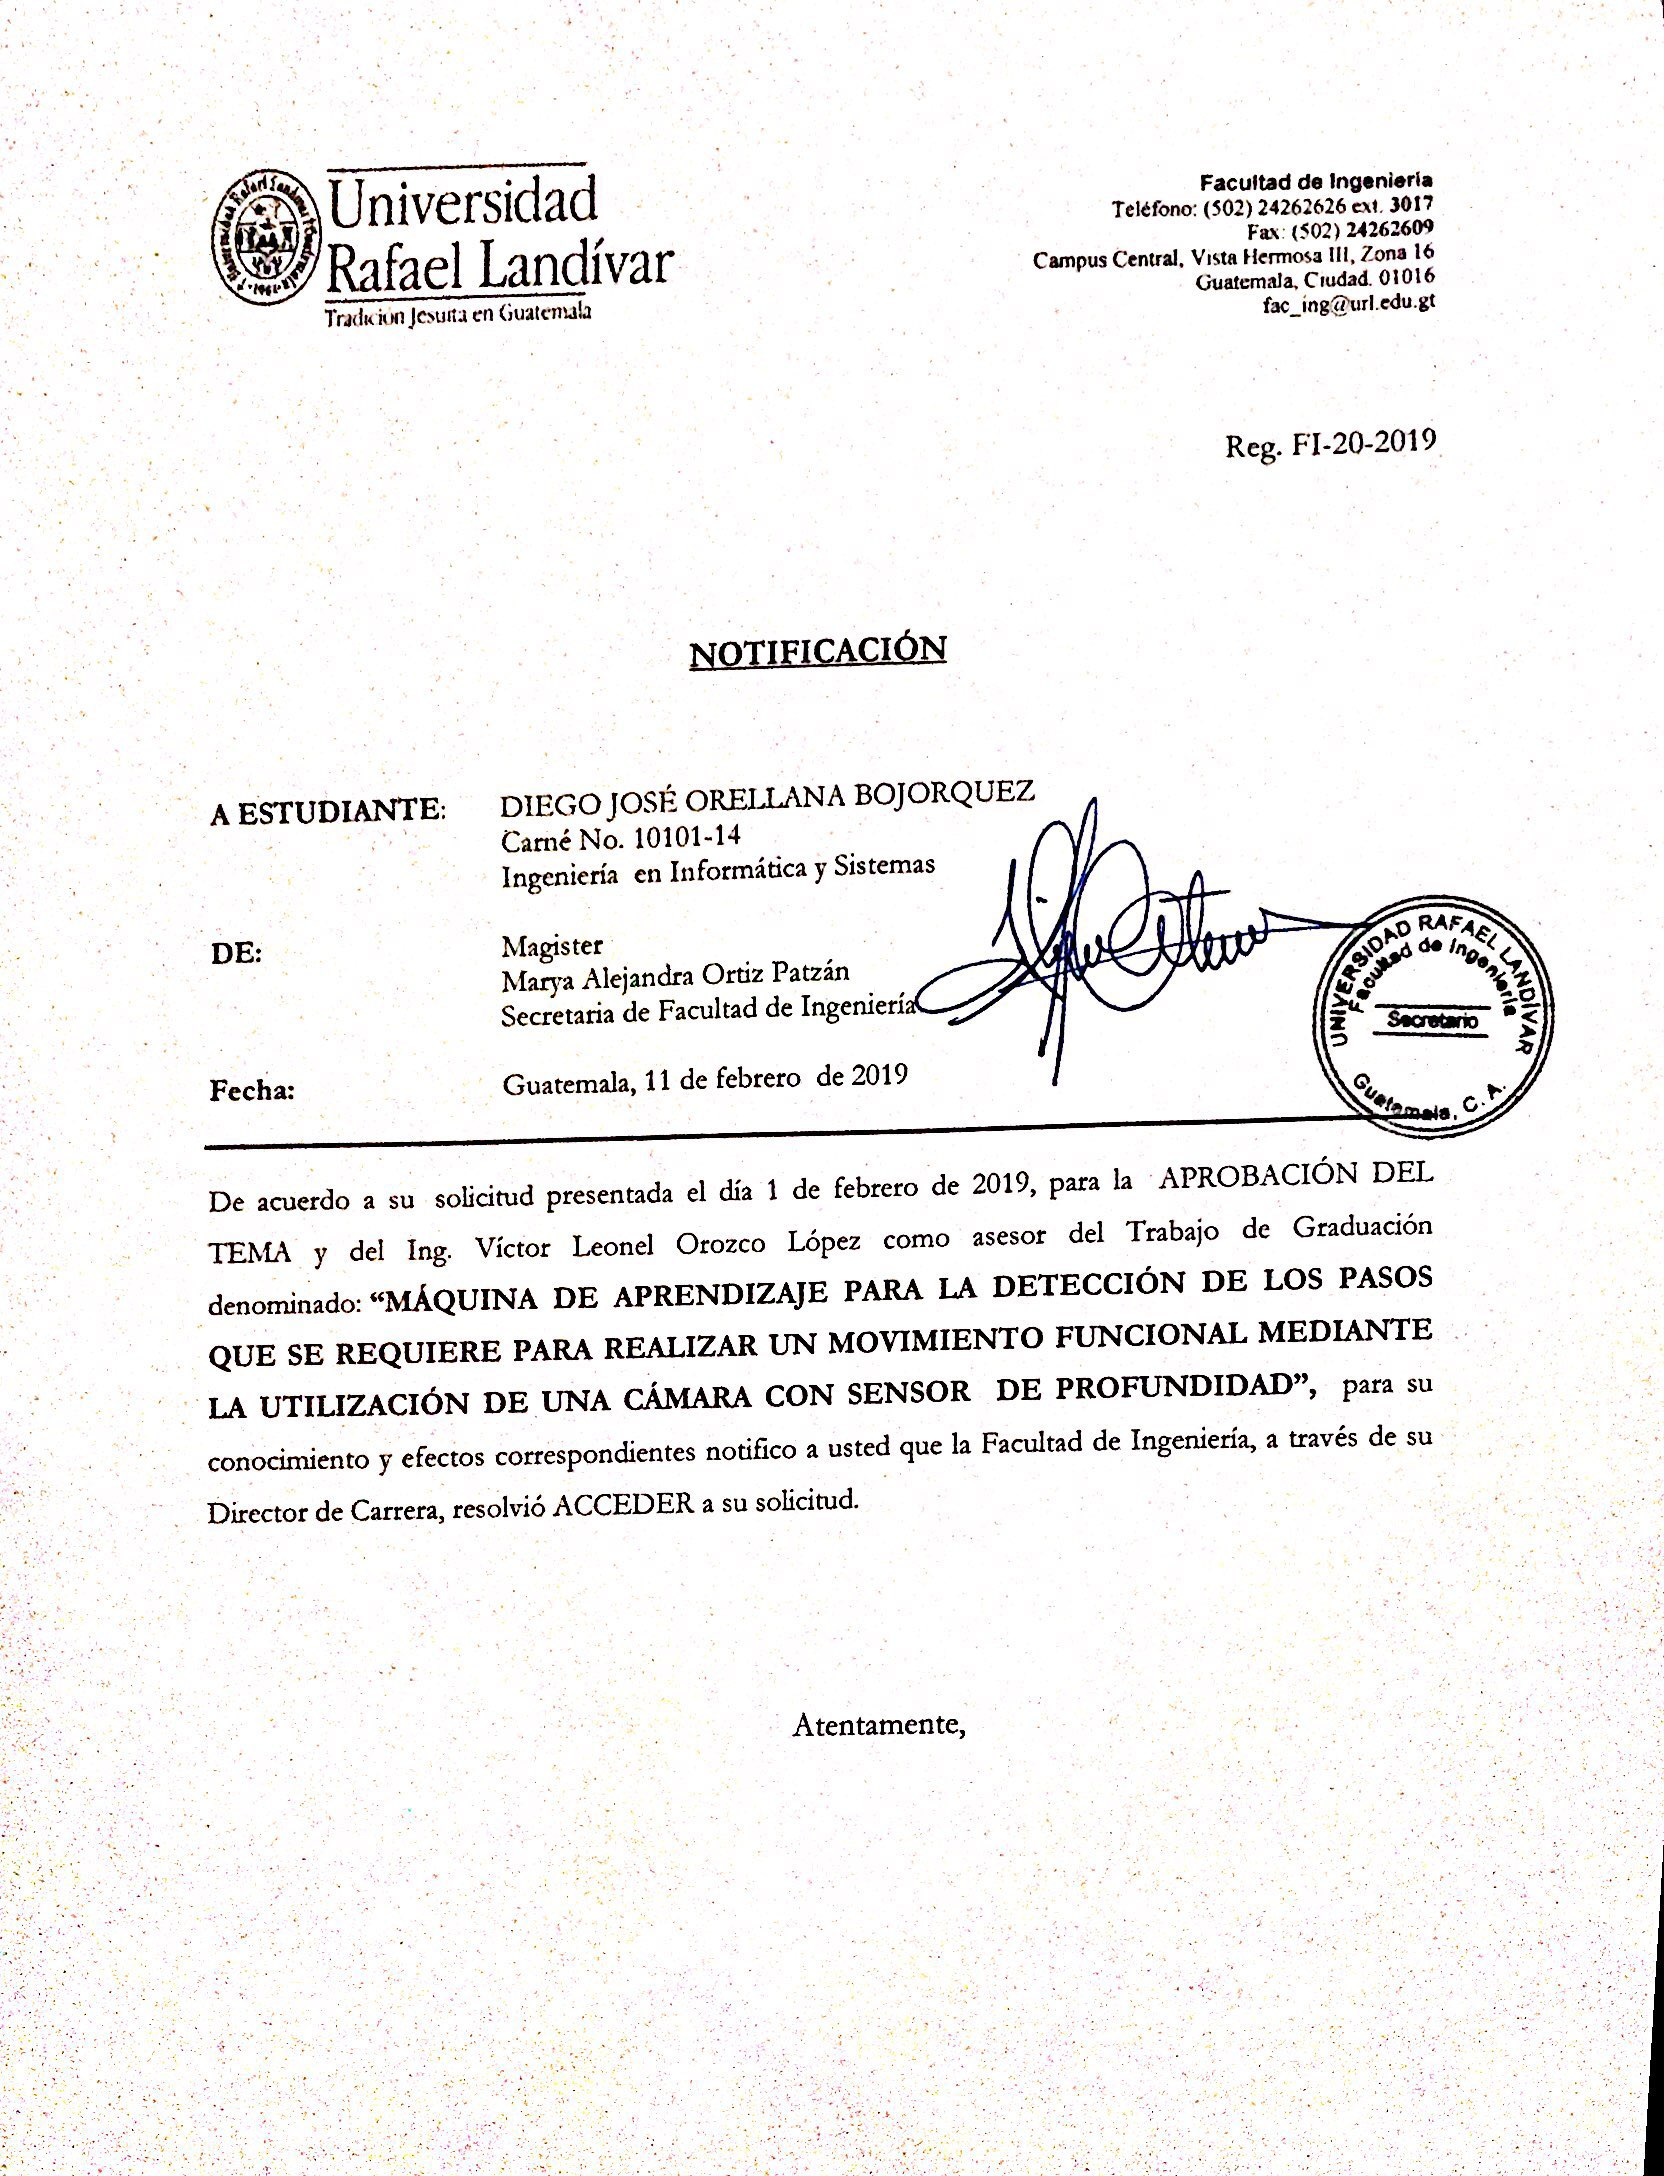
\includegraphics[width=18cm,height=22cm]{graphics/notificacion-tesis.jpg}
%%%%%%%%%%%%%%%%%%%%%%%%%%%%%%%%%%%%%%%%%%%%%%%%%
\afterpage{\blankpage}
\newpage
{\LARGE \textbf{Agradecimientos}}\\[2cm]
\begin{itemize}
\item A Dios, por ser alguien que me escucha en todo momento.
\item A mi mam\'a, gracias a ella he llegado tan lejos, adem\'as de estar siempre conmigo en las buenas y en las malas. 
\item A mi hermanos, por tenerme paciencia y confiar en m\'i en todo momento.
\item A mi pap\'a, por acompa\~narme siempre.
\item A mis amigos de la universidad, por ser una gran promoci\'on unida y apoyarnos en todo momento.
\item A mis amigos del colegio, por mantener nuestra amistad y vernos crecer.
\item Ingenieros Stanly Bola\~nos y Victor Orozco, por apoyarme en todo el proceso de trabajo de investigaci\'on.
\item Departamento de deportes de la universidad Rafael Land\'ivar, por confiar en mi proyecto de ingenier\'ia.
\end{itemize}
\begin{center}
Diego Orellana.
\end{center}
\afterpage{\blankpage}
\newpage
\tableofcontents.
\listoffigures.
\listoftables.
\listofcharts.
\listofformulas.
\listofcodes.
\mainmatter
% mainmatter/
%index
\afterpage{\blankpage}
\newpage
\chapter{Introducci\'on}
La Organizaci\'on Mundial de la Salud define la actividad f\'isica como cualquier movimiento producido por los m\'usculos esquel\'eticos, as\'i mismo est\'a definici\'on se relaciona al momento de que una persona realiza un ejercicio deportivo, debido que realiza una actividad f\'isica,  planificada, estructurada y repetitiva con el fin de objetivo de mejorar sus habilidades f\'isicas, entre ellas se pueden mencionar, la coordinaci\'on, la cual consta en combinar los pasos para ejecutar un movimiento v\'alido.
\medbreak
Por otra parte, la coordinaci\'on ha creado la modalidad de conteos de repeticiones de movimientos   v\'alidos, la cual se ha utilizado en actividades  deportivas, entre ellas est\'an el calentamiento previamente al entrenamiento, que consiste en realizar series de repeticiones de varios movimientos de calentamiento para preparar al cuerpo humano y evitar lesiones durante la rutina deportiva. De tal modo que es importante conocer como ejecutar un movimiento v\'alido.
\medbreak
Partiendo de conteos de repeticiones de movimientos v\'alidos, se ha creado este proyecto de ingenier\'ia, la cual consta en aplicar el algoritmo de Random Forest Regression por medio del software Visual Gesture Builder, que permite detectar los pasos de un movimiento v\'alido a trav\'es de la etiquetaci\'on de fotogramas de v\'ideos grabados por el sensor, Kinect V2.
\medbreak
Los v\'ideos consistir\'an en grabar repeticiones de un movimiento v\'alido ejecutados por atletas de un equipo deportivo de la Universidad Rafael Land\'ivar, en donde se centrar\'a en tres movimientos v\'alidos: La patada lateral del equipo de taekwondo, el saque derecha del equipo de tenis de mesa y finalmente el jumping jack del equipo de animaci\'on.
\medbreak
En cuanto al modelo de detecci\'on de los pasos de un movimiento v\'alido, proporcionar\'a un valor que representa la transici\'on del movimiento llamado factor del movimiento, esta variable ayudar\'a a comparar los valores de etiquetas y los  factores de movimientos de cada fotograma de un v\'ideo de prueba, con la finalidad de determinar el error del modelo y posteriormente utilizarla en los criterios de aceptaci\'on del modelo.
\medbreak
Si el modelo es aprobado, se crear\'a rangos de confianzas para detectar cada paso del movimiento a partir de la etiqueta y el error de cada paso. Posteriormente, el proyecto brindar\'a un algoritmo que clasifica un movimiento v\'alido, si durante una repetici\'on del movimiento, se detecta todos los pasos de manera ordenada.
\medbreak
En resumen, este proyecto aportar\'a en el \'area deportiva, con la finalidad de que diferentes deportes implemente su modelo de clasificaci\'on de los movimientos v\'alidos.
\newpage 
\section{Lo escrito sobre el tema} \label{tr}
\subsection{Sistema de detecci\'on y reconocimiento de la postura corporal basado en Kinect} \label{tr:1}
\citeA{pisharady2013kinect} mencionan que alrededor del 66\% de la poblaci\'on mundial  utilizan la comunicaci\'on no verbal, dicha comunicaci\'on esta conformado por posturas corporales, gestos, expresiones faciales y movimientos corporales. Por lo tanto, los autores propone un sistema para detectar expresiones est\'aticas -i.e. Posiciones que no cambian durante un per\'iodo de expresi\'on-.
\medbreak
Dicho sistema detecta y reconoce posturas corporales de una persona con la ayuda del sensor del Kinect, ya que le proporciona la posici\'on de las articulaciones del cuerpo humano -e.g. mano, codo, hombro, rodilla- en un espacio vectorial definido por el sensor. Posteriormente se calcula las caracter\'isticas angulares respecto a dos vectores de articulaciones, por ejemplo; para encontrar la caracter\'istica angular del codo derecho se utiliza los vectores de la mano derecha y hombro derecho.
\medbreak
Por otro lado, \citeA{pisharady2013kinect} analizaron un total de 11 componentes angulares para entrenar una \acrfull{SVM} de n\'ucleo polin\'omico, con la finalidad de detectar un total de 10 movimientos est\'aticos -e.g. Pararse, agacharse, hablar por tel\'efono-, as\'i mismo el entrenamiento consisti\'o en tomar 6000 muestras de posturas de 6 personas diferentes -i.e. Cada persona realiz\'o 100 muestras por postura-.
\medbreak
Finalmente, \citeA{pisharady2013kinect} recolectaron un total de 5000 muestras positivas (correspondiente a los 10 movimientos est\'aticos).  Como resultados obtuvieron una falla de pron\'ostico de 1.46\%, debido que el sensor Kinect no podr\'ia rastrear correctamente el seguimiento esqueleto.
\subsection{Reconstruci\'on de posturas en tiempo real} \label{tr:2}
\citeA{shum2013real} determinaron que el sensor Kinect tiene un problema con el reconocimiento de postura a la hora de interactuar con objetos externos -e.g. Baloncesto, levantamiento pesas-, por lo tanto, algunos datos de seguimiento de esqueleto son incorrecto, de tal manera que lo autores propone un m\'etodo para medir la confiabilidad de datos al momento de detectar una postura.
\medbreak
Para determinar el nivel de confiabilidad de datos, \citeA{shum2013real}, contruyeron una base de datos de 21590 posturas est\'aticas, la cual mide los \'angulos entre articulaciones. Esto permite  extraer las 30 posturas que se asemeja al movimiento real -i.e. 30 vecinos m\'as cercanos-.  Posteriormente, localizan cada postura en un nuevo espacio vectorial -i.e Espacio diferente al Kinect-, seleccionando as\'i la postura que tenga la menor distancia entre los puntos vectoriales.
\medbreak
Finalmente, \citeA{shum2013real}, realizaron las pruebas a 27 personas, dichas pruebas consist\'ia en hacer actividades con objetos externos -e.g. caja, silla, l\'apiz, pelota-, analizando la parte superior (Arriba de las caderas) e inferior de cada persona. Como resultados a estas pruebas, encontraron una diferencia de distancia de 9 a 13 cm entre la postura real y de referencia, determinando as\'i un nivel de confiabilidad del de 80\% respecto a dos sistemas de detecci\'on de movimiento en tiempo real \cite{shum2011fast,shum2012real}.
\subsection{Detecci\'on de posturas a la hora de sentarse para prevenir el s\'indrome de los trabajadores de oficina usando el Kinect} \label{tr:3}
\citeA{paliyawan2014prolonged} estudiaron el s\'indrome del trabajador de oficina, la cual consiste en un grupo de s\'intomas que tiene los trabajadores por los h\'abitos no saludables -e.g. La postura a la hora de sentarse-, provocando en la persona distintos dolores corporales.
\medbreak
En relaci\'on a los riesgos de salud de una persona, \citeA{paliyawan2014prolonged}, investigaron que una de las causas de una enfermedad no transmisible es debido al tiempo prolongado de estar sentado, sin realizar ning\'una actividad f\'isica. Por lo tanto, los autores  proponen un sistema que detecta las posturas a la hora que esta trabajando en una oficina.
\medbreak
Para realizar dicho sistema, \citeA{paliyawan2014prolonged} estudiaron las posturas de 28 personas,  recolectaron un total de 1326 posturas. De igual manera, cada postura conten\'ia un total 31 atributos -i.e. Tiempo y posici\'on de 10 articulaciones-. Posteriormente, el sistema procesa los datos y encuentra la \gls{diseuc} entre los datos consecutivos, permitiendo normalizar las distancias m\'aximas y m\'inimas por persona y en forma general -i.e. Conjunto de personas analizadas-.
\medbreak
Finalmente, el sistema detecta una buena o mala posici\'on, a partir de cuatros m\'etodos de clasificaci\'on: \gls{arbdec}, \gls{redneu}, \gls{bayesian} y 5 vecinos m\'as cercanos. Por lo tanto, para seleccionar el mejor m\'etodo, los autores realizaron una prueba a 10 personas, de tal manera que el mejor  clasificador es de \acrfull{KNN}, debido que tuvo una precisi\'on de  98.83\%. 
\subsection{Comparaci\'on de los m\'etodos de machine learning para el prop\'osito de la detecci\'on de la ca\'ida humana} \label{tr:4}
\citeA{stremy2014comparison}, estudian sobre la  ca\'ida en persona mayores, la cual determinaron que la ca\'ida  es el accidente m\'as peligros y frecuente que puede sufrir un anciano, debido que las personas de tercera edad se cae al menos una vez al a\~no y es la causa principal de muerte accidental en personas mayores de 65 a\~nos. Por lo tanto, los autores proponen un sistema que permite monitorear a los humanos y detectar posibles ca\'idas.
\medbreak
En relaci\'on a los datos del entrenamiento del sistema, los autores recolectaron un total de 450 actividades, realizada por 5 personas. As\'i mismo, clasificaron las actividades en tres movimientos est\'aticos: Parado, sentado y acostado. En cada movimiento est\'atico, obtiene la posici\'on de 20 articulaciones del cuerpo -e.g. Mano, codo, hombro-. Luego normaliza los datos a partir de la distancia desde el piso -i.e. Recta entre las articulaciones del p\'ie- a cada punto de articulaci\'on, con el fin objetivo de entrenar tres m\'etodos de clasificaci\'on: \gls{svmia}, \gls{bayesian} y \gls{arbdec}.
\medbreak
Para seleccionar el algoritmo clasificador, los autores realizaron 120 pruebas -i.e. 40 pruebas por cada movimiento est\'aticos-, en donde determinaron  que el \gls{arbdec} es la mejor opci\'on para ese proyecto, debido que tiene una exactitud de 93.3\% para detectar ca\'idas.
\subsection{Sistema de monitoreo de sue\~no usando el sensor Kinect} \label{tr:5}
\citeA{lee2015sleep} indican que hoy en d\'ia, la vida humana est\'a intensamente ocupada debido al constante trabajo y actividad, provocando en las personas el insomnio -i.e. Perdida del sue\~no-. As\'i mismo, el insomnio es conocido por discapacidades de aprendizaje y procesos ineficiente de trabajo. Por lo tanto, los autores presenta un sistema que recopila el movimiento y la postura durante el sue\~no.
\medbreak
Para calcular el movimiento de sue\~no, los autores tomaron la posici\'on de 19 articulaciones por cada medio segundo, posteriormente, el sistema calcula la \gls{diseuc} respecto a la posici\'on actual y anterior. Luego, suma todas las distancias de articulaciones para encontrar la distancia total y finalmente normaliza los datos, sumando todos los valores del movimiento respecto a una hora.
\medbreak
En relaci\'on en la detecci\'on de posturas, \citeA{lee2015sleep} separan el plano cartesiano en 6 cuadrantes, respecto a 3 l\'ineas gu\'ias: Linea media (articulaciones del Cuello y base de la columna vertebral), linea superior (Linea perpendicular a la articulaci\'on superior  de la columna vertebral) y la linea inferior (Linea perpendicular a la articulaci\'on base  de la columna vertebral). Posteriormente, localiza el cuadrante de las articulaciones de las manos y rodillas respecto a su ubicaci\'on, con el fin de objetivo de detectar 5 posiciones de sue\~no.
\medbreak
Finalmente para realizar las pruebas del sistema, reunieron a 20 estudiantes, en donde realizaron un monitoreo del sue\~no alrededor de 7 horas. La cual concluyeron que la perdida del sue\~no influye en el movimiento, debido que algunos estudiantes durmieron mal, ya que permanecieron en constante movimiento (Alrededor del 60 \% del  movimiento de sue\~no),
\subsection{Entrenador personal virtual a tr\'aves del sensor de Kinect} \label{tr:6}
\citeA{jin2015virtual} mencionan que el ejercicio es una de las actividades que se han pr\'acticado durante mucho tiempo, sin embargo, se ha ignorado debido al alto costo y el tiempo que se requiere -e.g. Ir al gimnasio-, adem\'as las aplicaciones o productos deportivos solo proporciona una gu\'ia deportiva y no existe una interacci\'on con los atletas. Por lo tanto los autores proporciona un entrenador virtual que brinda una gu\'ia de entrenamiento y una evaluaci\'on en tiempo real durante la actividad f\'isica de los usuarios.
\medbreak
La gu\'ia de entrenamiento consiste en una base de datos que identifica las acciones est\'aticas. Cada acci\'on es analizada como un modelo discreto de la aplicaci\'on, Visual Gesture Builder, posteriormente analiza la trayector\'ia  respecto a dos movimientos est\'aticas, en donde calcula las distancias euclidianas en relaci\'on a la posici\'on actual y anterior -i.e. Frame capturado un segundo antes- por cada articulaci\'on del cuerpo.
\medbreak 
Posteriormente realizan una evaluaci\'on de tiempo real por medio del puntaje de salud, dicho puntaje consiste en asignar un peso y calcular la distancia de cada articulaci\'on del cuerpo en relaci\'on a la posici\'on real y la posici\'on gu\'ia -i.e. Movimiento est\'atico-.
\medbreak 
Finalmente para entrenar el sistema, \citeA{jin2015virtual} recopilan v\'ideos por cada movimiento de an\'alisis, recolectando una muestra  de movimientos realizadas por un profesional o atleta.
\subsection{Una comparaci\'on entre las t\'ecnicas heur\'isticas y de aprendizaje autom\'atico en la detecci\'on de ca\'idas con Kinect v2} \label{tr:7}
En la publicaci\'on, A Comparison Between Heuristic And Machine Learning Techniques In Fall Detection Using Kinect v2 \cite{amini2016comparison}, se compara 2 m\'etodos para detectar la posici\'on, velocidad y aceleraci\'on de un usuario al momento de que un usuario sufre de una ca\'ida.
\medbreak 
Seg\'un \citeA{amini2016comparison}, el primer m\'etodo se basa en la \gls{Heur} que aprovecha la funcionalidad del seguimiento de esqueleto, la cual consiste en analizar la distancia entre la articulaci\'on de la cabeza y el suelo -i.e. Recta respecto a las articulaciones de los p\'ies-, mientras que el segundo m\'etodo consiste en una m\'aquina de aprendizaje, usando la funcionalidad visual y constructor de gestos -i.e. Visual Gesture Builder del sensor Kinect-, la cual analiza el escenario y le asigna un color a las posibles fallas de ca\'idas.
\medbreak 
As\'i mismo, \citeA{amini2016comparison} mencionan que para el primer m\'etodo los datos se fueron determinando a partir de la ecuaci\'on escalar de un plano, mientras que en el segundo m\'etodo se utiliz\'o el algoritmo AdaBoostTrigger -i.e Modelo discreto de Visual Gesture Builder-.
\medbreak 
Finalmente, \citeA{amini2016comparison} realizaron una prueba con 11 personas, la cual concluyeron que para el primer m\'etodo detectaba un 95.42\% de las ca\'idas, mientras que para el segundo m\'etodo fue de 88.33\%, por lo tanto seleccionaron el primer modelo.
\subsection{Sistema de detecci\'on de posiciones de un humano en tiempo real} \label{tr:8} 
En la publicaci\'on, Machine learning for real time poses classification using Kinect skeleton data \cite{choubik2016machine}, habla sobre el desarrollo de un sistema que reconoce 18 posiciones distintas del ser humano.
\medbreak 
Para construir el sistema,  \citeA{choubik2016machine} comparan cuatros modelos matem\'aticos: El primer modelo consist\'ia en una \gls{svmia} que consiste en encontrar un margen \'optimo dentro del espacio vectorial, con la finalidad de separar correctamente los datos. Dicho modelo se compara tres funciones del Kernel: Lineal, Polinomial y de \gls{brad} (RBF). As\'i mismo, el segundo modelo matem\'atico era una \gls{redneu} de dos funciones distintas: \gls{sigm}  y \gls{gaus}. De igual manera, el tercer modelo consiste en implementar el modelo \gls{knnia}, que determina la distancia de cada punto vectorial con su respectiva etiqueta y se ajusta un valor K, seg\'un el entrenamiento de datos. Finalmente el cuarto modelo consist\'ia en un , \gls{bayesian} la cual pronostica la posici\'on dado el punto vectorial.
\medbreak 
Igualmente, \citeA{choubik2016machine} entrenaron el sistema con 1800 datos, por cada dato se determin\'o  20 distancias relativa entre dos puntos de articulaci\'on -e.g. la altura entre codo derecho y hombro derecho-.
\medbreak 
Como resultados de las pruebas,  \citeA{choubik2016machine} seleccionaron el algoritmo lineal-SVM, debido que tiene un 99.05\% de precisi\'on.
\subsection{Sistema que detecta pasos de bailes k-pop} \label{tr:9} 
En la publicaci\'on, Classification of K-Pop Dance Movements Based on Skeleton Information Obtained by a Kinect Sensor \cite{kim2017classification}, habla sobre el Desarrollo de un sistema que reconoce 800 movimientos de baile de K-Pop.
\medbreak 
En relaci\'on al reconocimiento de bailes, el sistema identifica los 6 principales \'angulos de movimiento del cuerpo -i.e. Componente principal para el an\'alisis-, posteriormente determina la \gls{matcov}, la cual determina el valor de variaci\'on respecto a cada componente de an\'alisis,  esto permite obtener un an\'alisis discriminante lineal -i.e. Que tan dispersos se encuentra los valores-.
\medbreak 
Luego ingresa los datos de dispersi\'on para entrenar una  \acrfull{ELM}, y obtener una mayor exactitud en las respuesta en tiempo real.
\medbreak 
Finalmente, \citeA{kim2017classification} recolectaron un total de 1656 datos de entrenamiento por cada movimiento de baile, dichos datos fueron utilizado para entrenar tres modelos matem\'aticos: el primer modelo consist\'ia en un KNN, la cual reconoc\'ia entre 88\% a 92\% de los pasos de baile. El segundo modelo consist\'ia en un SVM, la cual detectaba entre 62\% a 84\% de los pasos de baile y finalmente el tercer modelo consist\'ia en una \gls{elmia}, la cual reconoc\'ia entre 75\% a 95\% de los bailes.
\medbreak 
Por lo cual, \citeA{kim2017classification}  seleccionaron el modelo ELM, debido que el modelo reconoce un porcentaje mayor de pasos de baile, as\'i mismo indica que el \'exito de reconocimiento de baile es debido la extracci\'on principal de componentes de datos -i.e. \'Angulos de cuerpo-, la reducci\'on de los datos y finalmente  el dise\~no clasificador.
\subsection{Comparaci\'on de trabajos relacionados} \label{tr:10}
Tal como se muestra en la tabla de la siguiente p\'agina, el sensor Kinect se ha utilizado para controlar algunos problemas de salud, a partir de distintos m\'etodos de clasificaci\'on entrenados por  movimientos est\'aticos. -e.g. \'Arboles de decisiones, KNN, Adaptive Boosting-. Por lo tanto para el presente proyecto, el movimiento flu\'ido se analiza por varios movimientos est\'aticos -i.e. Pasos del movimiento-, la cual se etiqueta con un valor decimal establecido por el modelo Random Forest Regresssion de Visual gesture Builder, de modo que se obtenga un factor de movimiento -i.e. Valor n\'umerico que representa la transici\'on que tiene el movimiento-. As\'i mismo se utiliza este modelo de clasificaci\'on debido que toma en consideraci\'on distintas variables del movimiento cinem\'aticos -e.g. Posici\'on, velocidad, desplazamiento, \'angulos de movimiento, Fuerza, torque muscular-, que son capturados por medio de v\'ideos de rutinas deportivas -i.e. Atletas que realizan series de repeticiones del movimiento-.
\medbreak
Igualmente los trabajos relacionados tiene en com\'un el proceso de la recolecci\'on de los datos, debido que selecciona articulaciones de estudio, lo cual para el presente proyecto se elige la articulaci\'on de an\'alisis, cuya funci\'on es medir la distancia de profundidad adecuada para ejecutar correctamente el seguimiento de esqueleto, adem\'as del conjunto de articulaciones que interviene para realizar un movimiento.
\medbreak
Por otro lado, este trabajo de investigaci\'on es distinto a los otros trabajos relacionados, debido que es un proyecto que se enfoca a verificar si una persona esta movi\'endose para satisfacer la actividad f\'isica necesaria por medio de repeticiones de un movimiento deportivo -e.g. Saltos, patadas, sentadillas-, con la ayuda del API del sensor Kinect y herramientas complementarias que permite crear modelos de detecci\'on de movimientos -e.g. Kinect Studio, Visual Gesture Builder-.
\begin{landscape}
\begin{table}[H]
\begin{center}
\caption{Comparaci\'on de trabajos relacionados con el sensor Kinect}
\label{tab:comTR}
\begin{tabular}{|l|l|l|l|l|l|}
\hline
Trabajo & A\~no & Enfoque & Objetivo & \begin{tabular}[c]{@{}l@{}}M\'etodo de\\ clasificaci\'on\end{tabular} & \begin{tabular}[c]{@{}l@{}}Cantidad\\ de datos\end{tabular} \\ \hline
\begin{tabular}[c]{@{}l@{}}Sistema de detecci\'on y reconocimiento de la \\ postura corporal basado en Kinect\end{tabular} & 2013 & Social & \begin{tabular}[c]{@{}l@{}}Reconocimiento de \\ comunicaci\'on no verbal\end{tabular} & \begin{tabular}[c]{@{}l@{}}SVM:\\ Lineal\end{tabular} & \begin{tabular}[c]{@{}l@{}}600  por\\ movimiento\end{tabular} \\ \hline
\begin{tabular}[c]{@{}l@{}} Reconstruci\'on de posturas en tiempo real \end{tabular} & 2013 & Tecnolog\'ia & \begin{tabular}[c]{@{}l@{}}Reconocimiento de \\ posturas con objetos \\ externos.\end{tabular} & \begin{tabular}[c]{@{}l@{}}30 vecinos \\ m\'as\\ cercanos\end{tabular} & \begin{tabular}[c]{@{}l@{}}3600 por\\ movimiento\end{tabular} \\ \hline
\begin{tabular}[c]{@{}l@{}} Detecci\'on de posturas a la hora de sentarse \\ para prevenir el s\'indrome de los trabajadores \\ de oficina usando el Kinect \end{tabular} & 2014 & Salud & \begin{tabular}[c]{@{}l@{}}Prevenci\'on del sindrome \\ de los trabajadores de \\ oficina\end{tabular} & \begin{tabular}[c]{@{}l@{}}5 vecinos \\ m\'as\\  cercanos\end{tabular} & \begin{tabular}[c]{@{}l@{}}1323 \\ posturas\end{tabular} \\ \hline
\begin{tabular}[c]{@{}l@{}} Comparaci\'on de los m\'etodos de machine \\ learning para el prop\'osito de \\ la detecci\'on de la ca\'ida humana \end{tabular} & 2014 & Salud & \begin{tabular}[c]{@{}l@{}}Detecci\'on de ca\'idas de \\ persona de tercera edad\end{tabular} & \begin{tabular}[c]{@{}l@{}}\'Adaptive\\ Boosting\end{tabular} & \begin{tabular}[c]{@{}l@{}}450 \\ posturas\end{tabular} \\ \hline
\begin{tabular}[c]{@{}l@{}} Sistema de monitoreo de sue\~no usando el sensor \\ Kinect \end{tabular} & 2015 & Salud & \begin{tabular}[c]{@{}l@{}}Monitoreo de  posiciones\\ y movimientos del sue\~no\end{tabular} & \begin{tabular}[c]{@{}l@{}}Clasificaci\'on \\ est\'atica\end{tabular} & \begin{tabular}[c]{@{}l@{}}  8 horas\\ por persona\end{tabular} \\ \hline
\begin{tabular}[c]{@{}l@{}} Entrenador personal virtual a tr\'aves del sensor \\ de Kinect \end{tabular} & 2015 & Deporte & Evaluaci\'on y gu\'ia deportiva & \begin{tabular}[c]{@{}l@{}}Adaptive\\ Boosting\end{tabular} & \begin{tabular}[c]{@{}l@{}}3 Movimientos\\ din\'amicos\end{tabular} \\ \hline
\begin{tabular}[c]{@{}l@{}} Una comparaci\'on entre las t\'ecnicas heur\'isticas \\ y de aprendizaje autom\'atico en la detecci\'on \\ de ca\'idas con Kinect v2 \end{tabular} & 2016 & Salud & \begin{tabular}[c]{@{}l@{}}Detecci\'on de ca\'idas con\\ objetos externos\end{tabular} & \begin{tabular}[c]{@{}l@{}}\'arboles de\\ decisiones\end{tabular} & \begin{tabular}[c]{@{}l@{}}29 minutos de\\ v\'ideo\end{tabular} \\ \hline
\begin{tabular}[c]{@{}l@{}} Sistema de detecci\'on de posiciones de \\ un humano en tiempo real \end{tabular} & 2016 & Tecnolog\'ia & \begin{tabular}[c]{@{}l@{}}Mejora en las posiciones\\ est\'aticas de una persona\end{tabular} & \begin{tabular}[c]{@{}l@{}}SVM\\ Lineal\end{tabular} & \begin{tabular}[c]{@{}l@{}}1800\\ movimientos\end{tabular} \\ \hline
\begin{tabular}[c]{@{}l@{}} Sistema que detecta pasos de bailes k-pop \end{tabular} & 2017 & Deporte & \begin{tabular}[c]{@{}l@{}}Detecci\'on de movimientos\\ de bailes\end{tabular} & \begin{tabular}[c]{@{}l@{}}m\'aquina\\ de aprendizaje\\ extremo\end{tabular} & \begin{tabular}[c]{@{}l@{}}1656 por\\ baile\end{tabular} \\ \hline
\end{tabular}
\end{center}
\textbf{Fuente:} Elaborado por el autor de tesis
\end{table}
\end{landscape}
\section{MARCO TE�RICO}
\subsection{C\'AMARA CON SENSOR DE PROFUNDIDAD}
Seg�n el estudio, On the performance of the Intel SR300 depth camera: metrological and critical characterization \cite{carfagni2017performance}, menciona que unas de las principales funciones de las \acrfull{RGBD} es adquirir y procesar datos en \acrfull{TRESD}, estas c�maras se han utilizado en el sector industrial y acad�mico en aplicaciones tales como: La localizaci�n y mapeo simult�neos, ingenier�a inversa y reconocimiento de posiciones y gestos. \\
Por otro lado el estudio, RGB-D mapping: Using Kinect-style depth cameras for dense 3D modeling of indoor environments   \cite{henry2012rgb}, indica que las c�maras con sensor de profundidad capturan \gls{pixeles} de informaci�n de im�genes (RGB) y de profundidad, tal como se muestra en la siguiente figura:
\begin{figure}[h]
	\caption{Captura de datos de una c�mara con sensor de profundidad}
	\label{fig:RGBD}
	\centering
	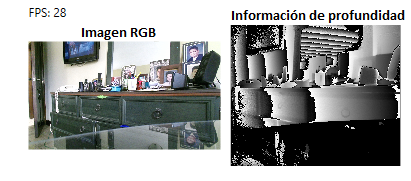
\includegraphics[]{graphics/RGB-D.PNG} \\
	\textbf{Fuente:} Tomado por el autor de tesis
\end{figure}  \\
La figura \ref{fig:RGBD}, fue capturado por el dispositivo, Kinect de XBox One, a una velocidad de 28 \acrfull{FPS}, cabe mencionar que los p�xeles  blancos de la imagen de la derecha, no se puede determinar el valor de profundidad, debido que falta el an�lisis de distancia, angulo relativo de la superficie, material de superficie, y otras variable m�s que se indicar� en el presente trabajo.
\subsubsection{Dispositivos en el mercado}
A continuaci�n se presentar� una lista de c�maras con sensor de profundidad, que se encuentra en el mercado hoy en d�a:
\begin{itemize}
	\item \textbf{ASUS XtionPro Live:} la corporaci�n ASUSTeK Computer \cite{xtionAsus}, desarroll� una c�mara con sensor de profundidad e infrarrojo, que permite detectar profundidad adaptativa, imagen en color y flujo de audio. Estas caracter�sticas permite capturar la imagen, el movimiento y la voz en tiempo real de un usuario. 
	\item \textbf{Structure Sensor:} La empresa, Occipital inc \cite{structureOccipital}, implementa un sensor de estructura, que permite escanear personas, espacios, mapas y objetos en 3D. 
	\item \textbf{Intel RealSense cameras:} Seg�n la tecnolog�a Intel RealSense \cite{intelRealSense}, permite detectar una alta velocidad de cuadros (p�xeles), RGB de calidad y la mejor resoluci�n de profundidad, en soluciones de realidad virtual, realidad aumentada, rob�tica, drones y otras aplicaciones m�s..
	\item \textbf{Microsoft Kinect:} Seg�n el estudio, Microsoft Kinect Sensor and its effect	\cite{zhang2012microsoft}, menciona que el Kinect contiene un sensor de profundidad, una c�mara a color y una matriz de micr�fonos que permite capturar movimientos, reconocer caracter�sticas faciales, construir un modelo del cuerpo en 3D y reconocer sonidos.
\end{itemize}
Tal como se observa en el listado, todas las c�maras de RGB-D permite detectar caracter�sticas del ambiente, por lo cual a la hora de escoger una c�mara se debe tomar en cuenta las siguientes especificaciones:
\begin{itemize}
	\item \textbf{Alcance del sensor 3D:} Seg�n el art�culo cient�fico, Kinect depth sensor evaluation for computer vision applications \cite{andersen2012kinect}, menciona que el alcance del sensor 3D es la medida m�xima de profundidad (z) desde un objeto hasta el sensor de profundidad.
	\item \textbf{3D Resoluci�n:} Hace referencia a la cantidad de p�xeles de la imagen que se obtiene del sensor de \gls{infrarrojo}.
	\item \textbf{RGB Resoluci�n:} Hace referencia a la cantidad de p�xeles de colores de una imagen.
	\item \textbf{\acrfull{FOV}:} Hace referencia al �ngulo m�ximo que puede detectar la c�mara, respecto a la horizontal(x) y la vertical (y).
	\item \textbf{Conexi�n:} Hace referencia al puerto de entrada y salida de la c�mara.
\end{itemize}
A continuaci�n se presentar� una comparaci�n de especificaciones entre las c�maras de RGB-D, mencionadas anteriormente:
\begin{table}[H]
\begin{center}
\caption{Comparaci�n de especificaciones entre c�maras de RGB-D }
\label{tab:RGBD}
\begin{tabular}{|l|l|l|l|l|l|} 
\hline
\textbf{Caracter�sticas}                                                          & \begin{tabular}[c]{@{}l@{}}\textbf{ASUS}\\\textbf{XtionPro}\\\textbf{Live}\end{tabular}   & \begin{tabular}[c]{@{}l@{}}\textbf{Structure}\\\textbf{Sensor}\end{tabular}  & \begin{tabular}[c]{@{}l@{}}\textbf{Intel}\\\textbf{RealSense}\\\textbf{SR300}\end{tabular}  & \begin{tabular}[c]{@{}l@{}}\textbf{Microsoft}\\\textbf{Kinect}\\\textbf{Live}\end{tabular} & \begin{tabular}[c]{@{}l@{}}\textbf{Microsoft}\\\textbf{Kinect}\\\textbf{v2}\end{tabular}	  \\ 
\hline
\begin{tabular}[c]{@{}l@{}}\textbf{Alcance del}\\\textbf{ sensor 3D}\end{tabular} & 0.8 a 3.5 m                                                                               & 0.4 a 3.5m                                                                   & 0.2 a 1.5m                                                                                  & 1.8 a 3.5m                                                                                 & 1.3 a 3.5m                                                                                  \\ 
\hline
\textbf{3D Resoluci�n}                                                            &\begin{tabular}[c]{@{}l@{}}640x480\\30fps\end{tabular}                   & \begin{tabular}[c]{@{}l@{}}640x480\\30fps\end{tabular}     & \begin{tabular}[c]{@{}l@{}}640x480\\60fps\end{tabular}                    &\begin{tabular}[c]{@{}l@{}}320x240\\30fps\end{tabular}					& \begin{tabular}[c]{@{}l@{}}512x424\\30fps\end{tabular}                    \\ 
\hline
\begin{tabular}[c]{@{}l@{}}\textbf{RGB}\\\textbf{ Resoluci�n}\end{tabular}        &\begin{tabular}[c]{@{}l@{}}1280x1024\\30fps\end{tabular}                   & \begin{tabular}[c]{@{}l@{}}640x480\\30fps\end{tabular}     & \begin{tabular}[c]{@{}l@{}}1920x1080\\30fps\end{tabular}                    &\begin{tabular}[c]{@{}l@{}}640x480\\30fps\end{tabular}					& \begin{tabular}[c]{@{}l@{}}1920x1080\\30fps\end{tabular}                    \\ 
\hline
\textbf{FOV}                                                                      & 58�H, 45�V                                                                                & 58�H, 45�V                                                                   & 73�H, 59�V                                                                                  & 57�H, 43�V                                                                                 & 70�H, 60�V                                                                                  \\ 
\hline
\textbf{Conexi�n}                                                                 & USB 2.0                                                                                   & USB 2.0                                                                      & USB 3.0                                                                                     & USB 2.0                                                                                    & USB 3.0                                                                                     \\
\hline
\end{tabular}
\end{center}
\textbf{Fuente:} Desarrollo de una aplicaci�n interactiva con Intel RealSense \cite{molero2018desarrollo} y Evaluation of the spatial resolution accuracy of the face tracking system for kinect for windows v1 and v2 \cite{amon2014evaluation}
\end{table}
En la tabla \ref{tab:RGBD}, se puede determinar que la c�maras, Intel RealSense SR300 y Microsoft Kinect V2, destacan de las dem�s c�maras debido  que tiene una mayor resoluci�n del sensor RGB y un campo de visi�n m�s amplio, por lo cual para el presente proyecto se seleccionar� la c�mara Microsoft Kinect V2. 
\chapter{Planteamiento del problema}
Dentro del \'area deportiva, las personas realizan entrenamiento de alta intensidad de un movimiento, con el fin objetivo de mejorar las habilidades f\'isicas. Sin embargo, al momento de que una persona est\'a realizando un movimiento, se est\'a desarrollando su coordinaci\'on (habilidad f\'isica), la cual consta en combinar varios pasos de manera ordenada para ejecutar el movimiento, sin embargo esta habilidad f\'isica puede llegar a presentar 2 problemas:
\begin{itemize}
	\item El primer problema consta de un usuario nuevo que desconoce como ejecutar el movimiento.
	\item El segundo problema se compone de un usuario que conoce el movimiento, pero lo ejecuta de distinta manera.
\end{itemize} 
La primera problem\'atica se resuelve si los atletas y los entrenadores les ense\~nan al nuevo usuario los pasos requeridos para ejecutar un movimiento v\'alido, con la finalidad de que el nuevo usuario lo aprenda y lo entrene constantemente.
\medbreak
El segundo problema surge cuando el usuario cambia de lugar de entrenamiento, debido que puede presentar nuevos criterios para ejecutar los movimientos que ha aprendido hacer, y esto puede conlleva a crear una discusi\'on: ?`Es v\'alido el movimiento que se conoce?
\medbreak
\medbreak
As\'i mismo el segundo problema se ha encontrado en eventos deportivos en Guatemala, por ejemplo el evento Unleash Your Fitness \cite{unleash}, competencia que presenta la modalidad de conteos de repeticiones de movimientos, en donde ha surgido conflictos de contabilizaciones de repeticiones de  movimientos v\'alidos entre jueces y atletas.
\medbreak
\medbreak
En resumen, el presente proyecto implementa la tecnolog\'ia de Visual Gesture Builder (etiquetador de fotogramas del seguimiento del esqueleto) con la finalidad de aplicar el algoritmo Random Forest Regression, para determinar la coordinaci\'on en un valor num\'erico llamado factor del movimiento y al mismo tiempo responder la siguiente pregunta:
\medbreak
\medbreak
\begin{center}
\textbf{?`Es posible clasificar el movimiento de una persona durante una actividad f\'isica como v\'alido o inv\'alido?}
\end{center}
\section{OBJETIVOS}
\subsection{OBJETIVO GENERAL}
Realizar una m\'quina de aprendizaje demostrativa que registre el seguimiento de esqueleto (Skeletan traking) a trav\'es de una c\'amara con sensor de profundidad, seleccionando el mejor modelo matem\'atico, con la finalidad de detectar los pasos que se requiere para realizar un movimiento funcional.
\subsection{OBJETIVOS ESPEC�FICOS}
\begin{enumerate}[1.]
    \item Identificar la altura correcta de la c\'amara y la distancia entre el usuario y el dispositivo para detectar el seguimiento del esqueleto humano.
    \item Analizar los kits de desarrollo de software (SDK) que permite grabar v\'ideos, tomar fotograf\'ias y capturar el seguimiento de esqueleto a trav\'es de una c\'amara con sensor de profundidad.
    \item Crear una interfaz gr\'afica que capture los datos de los pasos que deben seguir para realizar un movimiento funcional.
    \item Recolectar y validar los datos de entrenamiento de los movimientos funcionales.
    \item Identificar y comparar distintos modelos matem\'ticos a partir de los datos recolectado.
    \item Seleccionar el mejor modelo matem\'atico a partir de su rendimiento algor\'itmico y menor porcentaje de falla.
    \item Validar el modelo matem\'atico. 
    \item Crear una interfaz gr\'afica que detecte los pasos que se deben seguir para realizar un movimiento funcional.
\end{enumerate}
\section{HIP�TESIS}
\section{Variables} \label{vr}
\subsection{Primer Objetivo} \label{vr:1o}
Por movimiento se debe enumerar las articulaciones que ayudan a un usuario a moverse, de igual manera, por cada movimiento se debe enumerar los pasos que se debe seguir para ejecutar la acci\'on -i.e. Repetici\'on del movimiento-.
\subsubsection{Variables dependientes} \label{vr:1o:dep}
\begin{enumerate}
	\item[A.] \textbf{Articulaciones del movimiento:}  Vector de enteros la cual se almacena el valor del enumerador, JointType, del SDK de  \citeA{microsoftJointKinect}.
	\item[B.] \textbf{N\'umeros de pasos}: Valor positivo, mayor a 1.
\end{enumerate}
	\begin{figure}[H]
	\caption{Variables dependientes del primer objetivo}
	\label{fig:vardep1}
	\centering
	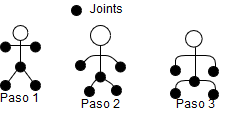
\includegraphics[width=300px,height=100px]{graphics/var-1obj.png} \\
	\textbf{Fuente:}Elaboraci\'on propia 
\end{figure}
\medbreak
\begin{table}[H]
\begin{center}
\caption{Definiciones de variables dependientes del primer objetivo}
\label{tab:def1o}
\begin{tabular}{|l|l|l|}
\hline
Enumeraci\'on & Definici\'on Operacional & Definici\'on conceptual \\
\hline
\ref{vr:1o:dep}.A & \begin{tabular}[c]{@{}l@{}}Son aquellas articulaciones\\ que interviene para realizar\\ el movimiento -i.e. Arcos\\ de movibilidad-.\end{tabular} & \begin{tabular}[c]{@{}l@{}}Conjunto de \'indices enteros \\ que representa las articulaciones\\ (ver figura \ref{fig:jointsKinect}) y arcos de\\ movibilidad (ver figuras \ref{fig:ArcosdeMovilidad} y \ref{fig:ArcosdeMovilidad2})\\ del seguimiento del esqueleto \end{tabular}  \\
\hline
\ref{vr:1o:dep}.B & \begin{tabular}[c]{@{}l@{}}Cantidad de pasos de an\'alisis\\ que tiene el movimiento\end{tabular} & \begin{tabular}[c]{@{}l@{}}De acuerdo a las variables del \\  movimiento (ver secci\'on \ref{mt:mf:var}), \\ los pasos define la coordinaci\'on \\ y balance del movimiento\end{tabular}\\
\hline
\end{tabular}
\end{center}
\textbf{Fuente:} Elaborado por el autor de tesis
\end{table}
\subsection{Tercer Objetivo} \label{vr:3o}
Por cada movimiento es necesario indicar la articulaci\'on de an\'alisis -i.e. Punto central de estudio-,  la cual a partir de ella se calcula la distancia de profundidad m\'inima y m\'axima, con la finalidad de que el seguimiento de esqueleto tenga un menor posible, sin embargo esta funcionalidad depende de la altura de usuario y el Kinect. 
\subsubsection{Variables dependientes} \label{vr:3o:dep}
\begin{enumerate}
	\item[A.] \textbf{Articulaci\'on de an\'alisis}: Valor entero que pertenece al  enumerador, JointType, del SDK de \citeA{microsoftJointKinect}. 
	\item[B.] \textbf{Altura del usuario}: Valor decimal positivo -i.e. Medida en metros- que se determina a partir de los componentes de altura de las articulaciones de la cabeza y p\'ies del usuario.	
	\begin{formula}[h]
	\centering
	\caption{Altura del usuario}
	\label{frm:alturaUser}
	\begin{equation}
y_{usuario}=y_{cabeza}-\frac{y_{pieDerecho}+y_{pieIzquierdo}}{2}
	\end{equation}
			\textbf{Fuente:} Planteado por el autor de tesis
\end{formula}  
	\item[C.] \textbf{Altura del kinect respecto al suelo}: Valor decimal positivo -i.e. Medida en metros- que permanece constante por movimiento. 
\end{enumerate}
\medbreak
\begin{figure}[H]
	\caption{Variables dependientes del tercer objetivo}
	\label{fig:vardep3}
	\centering
	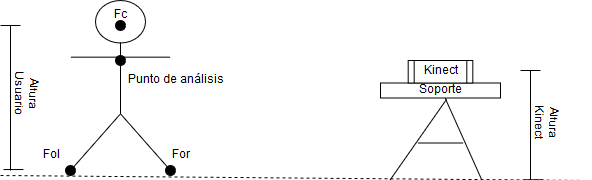
\includegraphics[width=300px,height=100px]{graphics/var-3obj.png} \\
	\textbf{Fuente:}Elaboraci\'on propia 
\end{figure}
\medbreak
\begin{table}[H]
\begin{center}
\caption{Definiciones de variables dependientes del Tercer objetivo}
\label{tab:def3o}
\begin{tabular}{|l|l|l|}
\hline
Enumeraci\'on & Definici\'on Operacional & Definici\'on conceptual \\
\hline
\ref{vr:3o:dep}.A & \begin{tabular}[c]{@{}l@{}}Articulaci\'on que ayuda\\ a determinar las distancias\\ m\'aximas y m\'inimas\\ de profundidad, adem\'as de\\ calcular el recorrido del atleta \\ durante la repetici\'on del movimiento\end{tabular} & \begin{tabular}[c]{@{}l@{}}Articulaci\'on del seguimiento de \\ de esqueleto (ver figura \ref{fig:jointsKinect}), que\\ permite realizar el an\'alisis del movimiento,\\ tal como se muestra en los trabajos \\ relacionados (Ver secci\'on \ref{tr}) \end{tabular}  \\
\hline
\ref{vr:3o:dep}.B & \begin{tabular}[c]{@{}l@{}}Variable de referencia para \\ ubicar al usuario en la profundidad \\ adecuada del seguimiento \\ del esqueleto\end{tabular} & \begin{tabular}[c]{@{}l@{}}La altura es una variable que puede \\ afectar los movimientos cinem\'aticos \\ (ver secci\'on \ref{mt:cam:kin}.\ref{mt:cam:kin:vgb}), \\ dado que afecta las dimenciones \\ del seguimiento de esqueleto\end{tabular}\\
\hline
\ref{vr:3o:dep}.C & \begin{tabular}[c]{@{}l@{}}Variable que permanece constante\\ por movimiento, adem\'as de ser \\ el punto central de  \\ captura de datos del Kinect\end{tabular} & \begin{tabular}[c]{@{}l@{}}La transmici\'on de datos del Kinect \\ (ver figura \ref{fig:interaccionKinect}) tendr\'a un menor error, \\  si se posiciona a la altura \\ en donde el sensor tenga un \\  mayor campo de visi\'on (ver figura \ref{fig:RGBESP} ) \end{tabular}\\
\hline
\end{tabular}
\end{center}
\textbf{Fuente:} Elaborado por el autor de tesis
\end{table}
\subsubsection{Variables independientes} \label{vr:3o:indep}
\begin{enumerate}
	\item[A.] \textbf{Distancia m\'inima de profundidad del movimiento}: Valor decimal positivo -i.e. Medida en metros- que determina la distancia m\'inima adecuada para ejecutar el seguimiento de esqueleto.
	\item[B.] \textbf{Distancia m\'axima de profundidad del movimiento}: Valor decimal positivo -i.e. Medida en metros- que determina la distancia m\'axima adecuada para ejecutar el seguimiento de esqueleto.
\end{enumerate}
\medbreak
\begin{figure}[H]
	\caption{Variables independientes del tercer objetivo}
	\label{fig:varindep3}
	\centering
	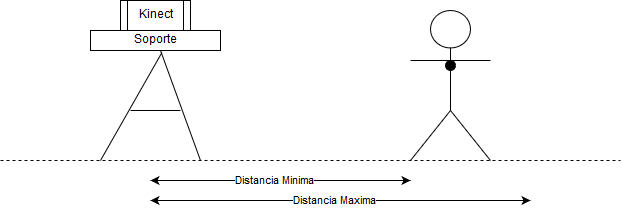
\includegraphics[width=300px,height=100px]{graphics/var-3obj-ind.png} \\
	\textbf{Fuente:}Elaboraci\'on propia 
\end{figure}
\medbreak
\begin{table}[H]
\begin{center}
\caption{Definiciones de variables independientes del Tercer objetivo}
\label{tab:def3o2}
\begin{tabular}{|l|l|l|}
\hline
Enumeraci\'on & Definici\'on Operacional & Definici\'on conceptual \\
\hline
\ref{vr:3o:indep}.A & \begin{tabular}[c]{@{}l@{}}Distancia m\'inima la\\ cual detecta todo el\\ esqueleto del usuario\\ -i.e. desde la cabeza \\ hasta los p\'ies-.\end{tabular} & \multirow{2}{*}{\begin{tabular}[c]{@{}l@{}} El seguimiento de esqueleto\\ depende del alcance del sensor \\ de profundidad y el campo \\ de visi\'on (ver figura \ref{fig:RGBESP}). \end{tabular}} \\
\cline{1-2}
\ref{vr:3o:indep}.B & \begin{tabular}[c]{@{}l@{}}Distancia m\'axima la\\ cual deja de detectar\\ todo el esqueleto del \\  usuario. \end{tabular} & \\
\hline
\end{tabular}
\end{center}
\textbf{Fuente:} Elaborado por el autor de tesis
\end{table}
\subsection{Cuarto Objetivo} \label{vr:4o}
Durante un movimiento, una articulaci\'on se desplaza con una direcci\'on - i.e. En todos los sentidos-, durante un per\'iodo de tiempo.
\subsubsection{Variables dependientes} \label{vr:4o:dep}
\begin{enumerate}
	\item[A.] \textbf{Tiempo de captura de datos}: Valor decimal positivo -i.e. Medida en segundos-, la cual mide el tiempo del movimiento de una articulaci\'on.
\end{enumerate}
\medbreak
\begin{figure}[H]
	\caption{Variables dependientes del cuarto objetivo}
	\label{fig:vardep4}
	\centering
	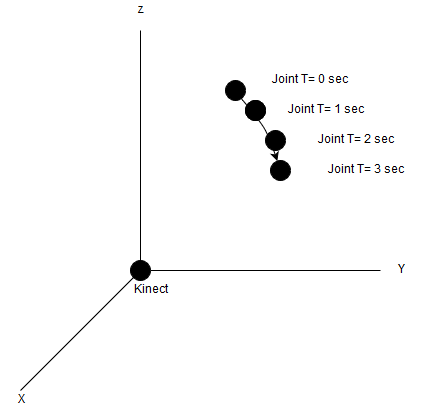
\includegraphics[width=180px,height=100px]{graphics/var-4obj.png} \\
	\textbf{Fuente:}Elaboraci\'on propia 
\end{figure}
\begin{table}[H]
\begin{center}
\caption{Definiciones de variables dependientes del cuarto objetivo}
\label{tab:def4o}
\begin{tabular}{|l|l|l|}
\hline
Enumeraci\'on & Definici\'on Operacional & Definici\'on conceptual \\
\hline
\ref{vr:4o:dep}.A & \begin{tabular}[c]{@{}l@{}}Unidad de tiempo \\  con respecto al \\ movimiento de an\'alisis\end{tabular} & \begin{tabular}[c]{@{}l@{}}De acuerdo a la resoluci\'on de 3D  \\ y del color (ver tabla \ref{tab:RGBD}), \\ el Kinect percibe un total \\ 30 frames por segundos, \\ lo cual puede llegar a  \\  capturar los datos cada \\  0.033 segundos. \end{tabular}  \\
\hline
\end{tabular}
\end{center}
\textbf{Fuente:} Elaborado por el autor de tesis
\end{table}
\subsubsection{Variables independientes} \label{vr:4o:indep}
\begin{enumerate}
	\item[A.] \textbf{Desplazamiento de la articulaci\'on}: Valor decimal positivo -i.e. Medida en metros- que determina la distancia de una articulac\'on y un punto de origen -i.e. Kinect-:
\begin{formula}[h]
	\centering
	\caption{desplazamiento de una articulaci\'on}
	\label{frm:desplazaUser}
	\begin{equation}
|r|=\sqrt{(x_{joint}-x_{o})^{2}+(y_{joint}-y_{o})^{2}+(z_{joint}-z_{o})^{2}}
	\end{equation}
	\textbf{Fuente:} Distancia euclediana \cite[p.~423]{ayres2001calculo}
\end{formula}  
	\item[B.] \textbf{Orientaci\'on de la articulaci\'on}: Vector de valores decimales positivo -i.e. Medida en radianes- que determina el \'angulo del desplazamiento con respecto a sus ejes.
\begin{formula}[h]
	\centering
	\caption{Orientaci\'on de una articulaci\'on}
	\label{frm:orientUser}
	\begin{equation}
Orientacion = [\alpha ,\beta ,\gamma ] = [cos^{-1}(\frac{x_{joint}}{|r|}),cos^{-1}(\frac{y_{joint}}{|r|}),cos^{-1}(\frac{z_{joint}}{|r|})]
	\end{equation}
	\textbf{Fuente:} \'Angulos directores de un vector \cite[p.~424]{ayres2001calculo}
\end{formula}  
\end{enumerate}
\medbreak
\begin{figure}[H]
	\caption{Variables independientes del cuarto objetivo}
	\label{fig:varIdep4}
	\centering
	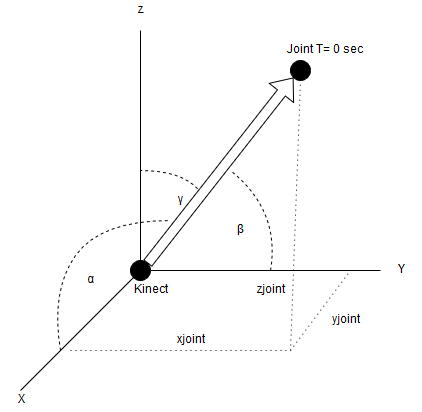
\includegraphics[width=230px,height=150px]{graphics/var-4obj-ind.png} \\
	\textbf{Fuente:}Elaboraci\'on propia 
\end{figure}
\begin{table}[H]
\begin{center}
\caption{Definiciones de variables independientes del cuarto objetivo}
\label{tab:def4oI}
\begin{tabular}{|l|l|l|}
\hline
Enumeraci\'on & Definici\'on Operacional & Definici\'on conceptual \\
\hline
\ref{vr:4o:indep}.A & \begin{tabular}[c]{@{}l@{}}Valor que muestra el desplazamiento \\ de la articulaci\'on de an\'alisis \\ -i.e. Como se esta \\ moviendo el cuerpo-. \end{tabular} & \begin{tabular}[c]{@{}l@{}}De acuerdo a las variables \\ de un movimiento (ver secci\'on \ref{mt:mf:var}) \\ y movimientos cin\'ematicos  \\ (ver secci\'on \ref{mt:cam:kin}.\ref{mt:cam:kin:vgb}),  \\ el desplazamiento permite calcular \\ la velocidad y aceleraci\'on \\ de un movimiento \\ a partir de la posici\'on  \\ de una articulaci\'on \\ (ver figura  \ref{fig:CoordenadaJoint})\\ con respecto al \\ tiempo de movimiento \end{tabular}  \\
\hline
\ref{vr:4o:indep}.B & \begin{tabular}[c]{@{}l@{}}Valor que muestra la direcci\'on   \\ de la articulaci\'on\end{tabular} & \begin{tabular}[c]{@{}l@{}}De acuerdo a las variables \\ de un movimiento (ver secci\'on \ref{mt:mf:var}), \\ la orientaci\'on permite tener mayor \\  precisi\'on y coordinaci\'on al \\  momento de ejecutar un \\  movimiento \end{tabular}  \\
\hline
\end{tabular}
\end{center}
\textbf{Fuente:} Elaborado por el autor de tesis
\end{table}
\subsection{Quinto Objetivo} \label{vr:5o}
Por cada movimiento se le debe asignar una etiqueta a cada paso, esto permite obtener el factor de movimiento -i.e. Pron\'ostico del modelo de reconocimiento de gesturas-.
\subsubsection{Variables dependientes} \label{vr:5o:dep}
\begin{enumerate}
	\item[A.] \textbf{Etiquetas}: Vector de valores decimales entre 0 a 1. Se debe tomar en cuenta que la diferencia entre dos etiquetas seguidas, es igual o cercano al valor de offset -i.e. Valor decimal que representa la distribuci\'on de pasos-.  
\end{enumerate}	
\medbreak
\begin{formula}[h]
	\centering
	\caption{Offset de etiquetas}
	\label{frm:offsetEt}
	\begin{equation}
offset = \frac{1}{pasos-1}
	\end{equation}
	\textbf{Fuente:} Propuesto por el autor de tesis
\end{formula}
\medbreak
\begin{formula}[h]
	\centering
	\caption{Asignaci\'on de etiquetas}
	\label{frm:vecEtiq}
	\begin{equation}
\begin{matrix}
etiquetas=[0, etiqueta(1), ..., etiqueta(paso), ..., 1],\; donde
\\
\\
etiqueta(paso) =
\left\{\begin{matrix}
0 & si\; es\; el\; primer \; paso
\\
etiqueta(paso-1)+offset & si\; es\; un\; paso\; intermedio
\\ 
1 & si\; es\; el\; ultimo\; paso
\end{matrix}\right.
\end{matrix}
	\end{equation}
	\textbf{Fuente:} Propuesto por el autor de tesis
\end{formula}  
\medbreak
\begin{figure}[H]
	\caption{Variables dependientes del quinto objetivo}
	\label{fig:vardep5}
	\centering
	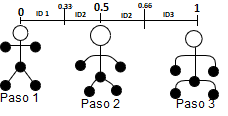
\includegraphics[width=180px,height=100px]{graphics/var-5obj.png} \\
	\textbf{Fuente:}Elaboraci\'on propia 
\end{figure}
\medbreak
\begin{table}[H]
\begin{center}
\caption{Definiciones de variables dependientes del quinto objetivo}
\label{tab:def5oI}
\begin{tabular}{|l|l|l|}
\hline
Enumeraci\'on & Definici\'on Operacional & Definici\'on conceptual \\
\hline
\ref{vr:5o:dep}.A & \begin{tabular}[c]{@{}l@{}}Valor que identifica \\ el paso de un movimiento. \end{tabular} & \begin{tabular}[c]{@{}l@{}}De acuerdo a las variables \\ de un movimiento (ver secci\'on \ref{mt:mf:var}) \\  los coordinaci\'on hace referencia \\ a las etiquetas del movimiento \\ (ver figura \ref{fig:modeloContinuo}). \end{tabular}  \\
\hline
\end{tabular}
\end{center}
\textbf{Fuente:} Elaborado por el autor de tesis
\end{table}
\subsubsection{Variables independientes} \label{vr:5o:indep}
\begin{enumerate}
	\item[A.] \textbf{Factor de movimiento}: valor  decimal entre 0 a 1, la cual representa la probabilidad del seguimiento de un movimiento.
\end{enumerate}	
\medbreak
\begin{figure}[H]
	\caption{Variables independientes del quinto objetivo}
	\label{fig:varIdep5}
	\centering
	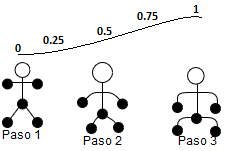
\includegraphics[width=180px,height=100px]{graphics/var-5obj-ind.png} \\
	\textbf{Fuente:}Elaboraci\'on propia 
\end{figure}
\medbreak
\begin{table}[H]
\begin{center}
\caption{Definiciones de variables independientes del quinto objetivo}
\label{tab:def5oI}
\begin{tabular}{|l|l|l|}
\hline
Enumeraci\'on & Definici\'on Operacional & Definici\'on conceptual \\
\hline
\ref{vr:5o:indep}.A & \begin{tabular}[c]{@{}l@{}}Valor que identifica \\ el seguimiento del movimiento \\ en tiempo real \end{tabular} & \begin{tabular}[c]{@{}l@{}}Variable que se calcula  \\ a partir del modelo Random  \\ Forest Regression (ver \\ seccio\'n \ref{mt:cam:kin}.\ref{mt:cam:kin:vgb}) \end{tabular}  \\
\hline
\end{tabular}
\end{center}
\textbf{Fuente:} Elaborado por el autor de tesis
\end{table}
\subsection{S\'eptimo Objetivo} \label{vr:7o}
Una rutina es configurada a partir de un n\'umero de series de tiempo de trabajo y descanso, en donde el usuario realiza las m\'aximas repeticiones posibles del movimiento  durante el tiempo de trabajo, tomando en cuenta que la repetici\'on debe pasar por todos los pasos definidos (ver variable \ref{vr:1o:dep}.B).
\subsubsection{Variables dependientes} \label{vr:7o:dep}
\begin{enumerate}
	\item[A.] \textbf{Tiempo de descanso}: Valor entero positivo -i.e. Medida en segundos-, la cual debe ser menor o igual al tiempo de trabajo.
	\item[B.] \textbf{Tiempo de Trabajo}: Valor entero positivo -i.e. Medida en segundos-.
	\item[C.] \textbf{Cantidad de series}: Valor entero positivo mayor a cero.
\end{enumerate}	
\begin{figure}[H]
	\caption{Variables dependientes del s\'eptimo  objetivo}
	\label{fig:vardep7}
	\centering
	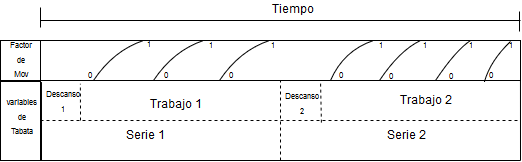
\includegraphics[width=300px,height=100px]{graphics/var-7obj.png} \\
	\textbf{Fuente:}Elaboraci\'on propia 
\end{figure}
\medbreak
\begin{table}[H]
\begin{center}
\caption{Definiciones de variables dependientes del s\'eptimo objetivo}
\label{tab:def7}
\begin{tabular}{|l|l|l|}
\hline
Enumeraci\'on & Definici\'on Operacional & Definici\'on conceptual \\
\hline
\ref{vr:7o:dep}.A & \begin{tabular}[c]{@{}l@{}}Valor que controla el \\ tiempo que debe descansar \\ un usuario durante \\ su rutina -i.e. No \\ se cuenta repeticiones-. \end{tabular} & \multirow{3}{*}{\begin{tabular}[c]{@{}l@{}}Estas variables son \\  definidas a partir de \\ la rutina, Tabata, debido \\ que es un entrenamiento controlado \\  de alta intensidad, \\ cuyo resultado es \\ una mayor metabolizaci\'on \\ del cuerpo  (ver secci\'on \ref{mt:mf:rut}.\ref{mt:mf:rut:hiit})\end{tabular}} \\  
\cline{1-2}
\ref{vr:7o:dep}.B & \begin{tabular}[c]{@{}l@{}}Valor que controla el \\ tiempo que debe trabajar \\ un usuario durante \\ su rutina -i.e. Realizar \\ las m\'aximas repeticiones-. \end{tabular} & \\  
\cline{1-2}
\ref{vr:7o:dep}.C & \begin{tabular}[c]{@{}l@{}}Valor que controla la \\ cantidad de tiempos de \\ trabajos y descanso \\ en una rutina. \end{tabular} &  \\  
\hline
\end{tabular}
\end{center}
\textbf{Fuente:} Elaborado por el autor de tesis
\end{table}
\subsubsection{Variables independientes} \label{vr:7oi:indep}
\begin{enumerate}
	\item[A.] \textbf{Detalle del paso}: Es un vector de valores n\'umericos, en donde contiene el factor de movimiento, n\'umero de paso y la matriz de articulaciones -i.e. Esqueleto-. 
	\item[B.] \textbf{Repetici\'on}:  Es un vector de detalle de todos los pasos definido por el movimiento.
\end{enumerate}	
\begin{formula}[h]
	\centering
	\caption{Matriz de variables independientes del s\'eptimo objetivo}
	\label{frm:vecEtiq}
	\begin{equation}
\begin{matrix}
i & enumerador\: de\: la\: articulacion \\ 
x & distancia\, horizontal \: (pixeles) \\ 
y & distancia\, vertical\: (pixeles) \\ 
joint_{i}& [i,x,y] \\ 
 & \\ 
esqueleto & \begin{bmatrix}
joint_{0} \\ 
... \\ 
joint_{i}\\ 
... \\ 
joint_{24}
\end{bmatrix}  \\ 
 & \\ 
fm & factor \, del \, movimiento \\ 
p  & paso \, del \,movimiento \\ 
step_{p}  & [fm,p,esqueleto, tiempo] \\
 & \\ 
Repeticion & [step_{0}, ...,  step_{col}, ..., step_{last}] \\
serie & [repeticion] \\
series & [serie]
\end{matrix}
	\end{equation}
	\textbf{Fuente:} Propuesto por el autor de tesis
\end{formula}  
\medbreak
\begin{table}[H]
\begin{center}
\caption{Definiciones de variables independientes del s\'eptimo objetivo}
\label{tab:defoi7}
\begin{tabular}{|l|l|l|}
\hline
Enumeraci\'on & Definici\'on Operacional & Definici\'on conceptual \\
\hline
\ref{vr:7oi:indep}.A & \begin{tabular}[c]{@{}l@{}}Variable que almacena informaci\'on \\ del esqueleto humano \\ -i.e. posici\'on de cada \\ articulaci\'on-, con respecto \\  a cada paso del movimiento  \end{tabular} &  \begin{tabular}[c]{@{}l@{}}El seguimiento de esqueleto \\ puede ser dibujado en \\ una imagen 2D (ver figura \ref{fig:skeletanTracking}), \\  la cual proporciona \\ la posici\'on de cada articulaci\'on, \\ con el fin objetivo  de \\ calcular la agilidad \\ del movimiento (ver secci\'on \ref{mt:mf:var})\end{tabular}\\
\hline
\ref{vr:7oi:indep}.B & \begin{tabular}[c]{@{}l@{}}Variable que almacena informaci\'on \\ de todos los pasos \\ en orden cronol\'ogico  \\ -e.g. la informaci\'on del paso 1 \\ es guardada antes del paso 2-. \\ Se debe tomar en cuenta \\ que la repetici\'on ser\'a \\ contable, si tiene todos \' los pasos  \end{tabular} & \begin{tabular}[c]{@{}l@{}}Variable que permite \\ contabilizar la actividad \\ f\'isica de una persona  \\  (ver secci\'on \ref{mt:af:var})\end{tabular}\\  
\hline
\end{tabular}
\end{center}
\textbf{Fuente:} Elaborado por el autor de tesis
\end{table}
\subsection{Octavo Objetivo} \label{vr:8o}
En cada paso del movimiento, los m\'usculos se mueve a partir del arco del  movilidad. 
\subsubsection{Variables independientes} \label{vr:8oi:indep}
\begin{enumerate}
	\item[A.] \textbf{Flexibilidad}: Valor decimal positivo -i.e. Medida en grados-, la cual mide el \'angulo de una articulaci\'on respecto a 2 articulaciones continuas.
\end{enumerate}	
\begin{figure}[H]
	\caption{Variables independiente del octavo  objetivo}
	\label{fig:varidep8}
	\centering
	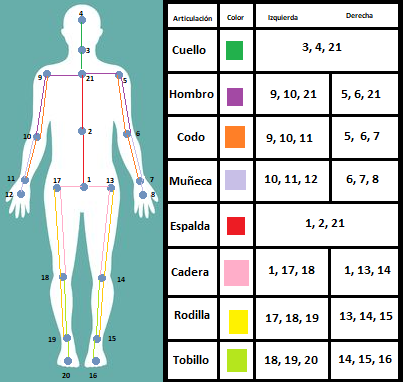
\includegraphics[width=280px,height=180px]{graphics/EskeletanAngles.png} \\
	\textbf{Fuente:}Elaboraci\'on propia 
\end{figure}
\begin{formula}[h]
	\centering
	\caption{Rotaci\'on a un punto de articulaci\'on}
	\label{frm:rotEq}
	\begin{equation}
\begin{matrix}
arco_{a} = [joint_{a},joint_{b},joint_{c}]\\ 
joint_{b}^{'} = [a,joint_{b}x-joint_{a}x, joint_{b}y-joint_{a}y]\\ 
joint_{c}^{'} = [a,joint_{c}x-joint_{a}x, joint_{c}y-joint_{a}y]
\end{matrix}
	\end{equation}
	\textbf{Fuente:} Traslaci\'on de ejes \cite[p.~982]{aguilar2009matematicas}
\end{formula}  
\begin{formula}[h]
	\centering
	\caption{flexibilidad de una articulaci\'on}
	\label{frm:angleArc}
	\begin{equation}
\begin{matrix}
joint_{b}^{'} \cdot joint_{c}^{'}=  joint_{b}^{'}x \, joint_{c}^{'}x + joint_{b}^{'}y \, joint_{c}^{'}y \\ 
\\ 
\left | joint \right |= \sqrt{ {joint_{x}}^{2} + {joint_{y}}^{2}}\\ 
\\ 
\alpha _{arco_{a}} = \frac{joint_{b}^{'} \cdot joint_{c}^{'}}{\left | joint_{b}^{'}\right |\left |  joint_{c}^{'}\right |}
\end{matrix}
	\end{equation}
	\textbf{Fuente:} \'Angulo entre dos vectores \cite[p.~591]{stewart2013precalculus}
\end{formula}  
\begin{table}[H]
\begin{center}
\caption{Definiciones de variables independientes del octavo objetivo}
\label{tab:defoi8}
\begin{tabular}{|l|l|l|}
\hline
Enumeraci\'on & Definici\'on Operacional & Definici\'on conceptual \\
\hline
\ref{vr:8oi:indep}.A & \begin{tabular}[c]{@{}l@{}}Variable que permite realizar \\ el movimiento en las articulaciones \\ del cuerpo humano  \end{tabular} &  \begin{tabular}[c]{@{}l@{}}De acuerdo a las variables \\ de un movimiento (ver secci\'on \ref{mt:mf:var})\\ la flexibilidad ayuda a la precisi\'on,\\ balance y coordinaci\'on \\ de un movimiento\end{tabular}\\
\hline
\end{tabular}
\end{center}
\textbf{Fuente:} Elaborado por el autor de tesis
\end{table}
\section{Alcances y limitaciones}
\begin{itemize}
\item Se trabajar\'a con los equipos deportivos que entrenan dentro de la Universidad Rafael Land\'ivar.
\item Se instalar\'a el prototipo de toma de datos del proyecto, en los lugares de entrenamiento de cada equipo deportivo.
\item En cada lugar de entrenamiento debe haber una fuente de energ\'ia para conectar la computadora port\'atil y el sensor Kinect.
\item Cada deporte de la Universidad Rafael Land\'ivar, trabajan  3 d\'ias de entrenamiento competitivo (combates, partidos, rutinas) y un d\'ia de entrenamiento de aprendizaje (e.g. t\'ecnicas, movimientos, dominio). Por lo tanto, se recolectar\'a los datos durante el entrenamiento de aprendizaje de cada deporte.
\item Se utilizar\'a un sensor Kinect, la cual se posicionar\'a de manera que genere completamente el seguimiento del esqueleto.
\item Por cada deporte seleccionado, se analizar\'a un movimiento que no salga del campo de visi\'on del sensor Kinect.
\item Antes de la captura de datos, el atleta debe realizar el calentamiento que realiza constantemente.
\item Durante todas las etapas, el atleta debe estar en un entorno adecuado y as\'i mismo con la vestimenta correcta (e.g. Ropa deportiva).
\item Debe estar presente el entrenador o profesional, durante la captura de datos.
\item  La captura de datos se realizar\'a de manera individual (Atleta por atleta).
\item  La recolecci\'on de datos se centra en el seguimiento del esqueleto del atleta.
\item La validaci\'on de datos se realizar\'a con los atletas que no participar\'an en la etapa de recolecci\'on de datos.
\item La actividad f\'isica se contabilizar\'a por medio de las repeticiones de un  movimiento, ejecutados durante una rutina tabata.
\item Las rutinas tabata ser\'an realizadas conjuntamente por el entrenador y el investigador.
\item Las aplicaciones que implemente el seguimiento del esqueleto ser\'an desarrolladas para el sistema operativo windows 10.
\item \'Unicamente se visualizar\'a los resultados de la rutina actual (no se llevar\'an los registros hist\'oricos de resultado de un atleta).
\end{itemize}
\section{Aportes}
El presente proyecto aporta un software que identifica si una persona esta en movimiento, con la ayuda de dos \'areas de estudios:
\begin{itemize}
	\item \textbf{\gls{visArt}:} La investigaci\'on brinda informaci\'on sobre el funcionamiento del sensor Kinect y sus respectivas herramientas, las cuales ayudan a crear una base de datos de reconocimiento de gesturas y posturas, usando la tecnolog\'ia de m\'aquinas de aprendizajes -i.e. Random Forest Regression-, con la finalidad de crear un modelo que detecta el movimiento de una persona.
	\item \textbf{Salud y deporte para el control del sedentarismo:} La investigaci\'on aporta tres movimientos que se puede ejecutar en rutinas de alta intensidad, que permite estimular el cuerpo humano para cumplir las recomendaciones de la organizaci\'on mundial de la salud.
\end{itemize}

\chapter{Metodolog\'ia}
La investigaci\'on se trabaj\'o con un enfoque mixto debido que integra dos m\'etodos:
\begin{itemize}
	\item \textbf{Cualitativo:} Dentro de la investigaci\'on se utiliz\'o el m\'etodo de observaci\'on para seleccionar el movimiento de an\'alisis por cada equipo deportivo, as\'i mismo el investigador realiz\'o grupos focales con los entrenadores y atletas de cada equipo deportivo, con la finalidad de documentar las formas correctas de realizar el movimiento analizado -e.g. Calentamientos, pasos del movimiento, ejercicios de estiramientos-.
	\item \textbf{Cuantitativo:} En este proyecto de ingenier\'ia se utiliz\'o el Kinect para tomar v\'ideos de atletas realizando el movimiento, en donde por cada captura de dato (fotograma), se recolect\'o los datos de las variables del movimiento cinem\'atico, con la finalidad de etiquetarlo con un valor decimal y crear un modelo de pron\'ostico del movimiento, as\'i mismo se  encontr\'o el m\'argen de error de cada modelo a partir de t\'ecnicas de estad\'isticas -e.g.  Ra\'iz del error cuadr\'atico medio-.
\end{itemize}
\section{Sujetos}
El departamento de deportes de la Universidad Rafael Land\'ivar, le proporcion\'o al investigador, la colaboraci\'on de todos los deportes -e.g. F\'utbol, voleibol, baloncesto, tenis, banda, zumba, atletismo, nataci\'on, taekwondo, tenis de mesa y animaci\'on-. Lo cual el investigador tuvo que realizar filtros para seleccionar la poblaci\'on, descartando aquellos deportes que entrenaban en las federaciones nacionales de Guatemala -i.e. Lugares externos a la Universidad Rafael Land\'ivar-, entre ellos estaban: Atletismo, nataci\'on y tenis. Por otro lado, el investigador apart\'o los deportes que se ejercitaban dentro de una cancha deportiva debido a la dificultad de colocar todos los materiales necesarios del proyecto para la toma de datos, por lo cual se elimin\'o los deportes de:  f\'utbol, voleibol y baloncesto. Finalmente, el investigador ignor\'o los deportes de banda y zumba, ya que son actividades que se trabajan en conjunto con otros departamentos de la Universidad Rafael Landivar -e.g. Unidad de artes Land\'ivar-. De modo que el investigador seleccion\'o los siguientes deportes:
\begin{itemize}
	\item \textbf{Tenis de mesa:} Deporte de raqueta que se juega sobre una mesa rectangular de manera individual o en parejas, con el fin objetivo de golpear una peque\~na pelota.
	\item \textbf{Animaci\'on:} Deporte grupal que combina la m\'usica y gimnasia, a partir de rutinas de baile que entusiasma un p\'ublico o evento deportivo.
	\item \textbf{Taekwondo:} Deporte individual basado en el arte marcial coreano moderno, que consiste en el uso de los pies, brazos y pu\~nos dentro de un combate.
\end{itemize}
\subsection{Primer tipo} \label{sj:1t}
Define la cantidad de sujetos que participaron en la colecta de los datos para la creaci\'on del modelo de reconocimiento del movimiento, a partir de tres fases distintas:
\begin{itemize}
	\item \textbf{Construcci\'on:} Atletas que construyeron el modelo continuo de la m\'aquina de aprendizaje.
	\item \textbf{Pruebas:} Muestra de usuarios que se emple\'o para el c\'alculo de los m\'argenes de  errores del pron\'ostico del modelo.
	\item \textbf{Validaci\'on:} Conjunto de deportistas que realizaron las pruebas al modelo en tiempo real.
\end{itemize}
\subsubsection{Equipo de animaci\'on de la Universidad Rafael Land\'ivar} \label{sj:1t:ani}
\begin{table}[H]
\begin{center}
\caption{Muestra del equipo de animadoras}
\label{tab:MuestraCheerleaders}
\begin{tabular}{lc}
\hline
\multicolumn{1}{|l|}{\textbf{Descripci\'on}} & \multicolumn{1}{l|}{\textbf{Cantidad}} \\ \hline
\multicolumn{1}{|l|}{Atletas para la construcci\'on del modelo} & \multicolumn{1}{c|}{6} \\ \hline
\multicolumn{1}{|l|}{Atletas para las pruebas del modelo} & \multicolumn{1}{c|}{1} \\ \hline
\multicolumn{1}{|l|}{Atletas para la validaci\'on del modelo} & \multicolumn{1}{c|}{2} \\ \hline
\multicolumn{1}{|r|}{Total de atletas} & \multicolumn{1}{c|}{9} \\ \hline
\textbf{Fuente:} Propia.
\end{tabular}
\end{center}
\end{table}
\subsubsection{Equipo de tenis de mesa de la Universidad Rafael Land\'ivar}\label{sj:1t:ten}
\begin{table}[H]
\begin{center}
\caption{Muestra del equipo de tenis de mesa}
\label{tab:MuestraTenis}
\begin{tabular}{lc}
\hline
\multicolumn{1}{|l|}{\textbf{Descripci\'on}} & \multicolumn{1}{l|}{\textbf{Cantidad}} \\ \hline
\multicolumn{1}{|l|}{Atletas para la construcci\'on del modelo} & \multicolumn{1}{c|}{5} \\ \hline
\multicolumn{1}{|l|}{Atletas para las pruebas del modelo} & \multicolumn{1}{c|}{1} \\ \hline
\multicolumn{1}{|l|}{Atletas para la validaci\'on del modelo} & \multicolumn{1}{c|}{3} \\ \hline
\multicolumn{1}{|r|}{Total de atletas} & \multicolumn{1}{c|}{9} \\ \hline
\textbf{Fuente:} Propia.
\end{tabular}
\end{center}
\end{table}
\subsubsection{Equipo de taekwondo de la Universidad Rafael Land\'ivar}\label{sj:1t:tae}
\begin{table}[H]
\begin{center}
\caption{Muestra del equipo de taekwondo}
\label{tab:MuestraTaekwondo}
\begin{tabular}{lc}
\hline
\multicolumn{1}{|l|}{\textbf{Descripci\'on}} & \multicolumn{1}{l|}{\textbf{Cantidad}} \\ \hline
\multicolumn{1}{|l|}{Atletas para la construcci\'on del modelo} & \multicolumn{1}{c|}{15} \\ \hline
\multicolumn{1}{|l|}{Atletas para las pruebas del modelo} & \multicolumn{1}{c|}{1} \\ \hline
\multicolumn{1}{|r|}{Total de atletas} & \multicolumn{1}{c|}{16} \\ \hline
\textbf{Fuente:} Observaci\'on del investigador durante el trabajo de campo.
\end{tabular}
\end{center}
\end{table}
\subsection{Segundo tipo} \label{sj:2t}
A continuaci\'on se muestra un organigrama de la estructura del departamento de deportes de la Universidad Rafael Land\'ivar, en ella se muestra todos los profesionales que aportaron en la investigaci\'on:
\begin{figure}[H]
	\caption{Organigrama del departamento de deportes de la Universidad Rafael Land\'ivar}
	\label{fig:orgDeportes}
	\centering
	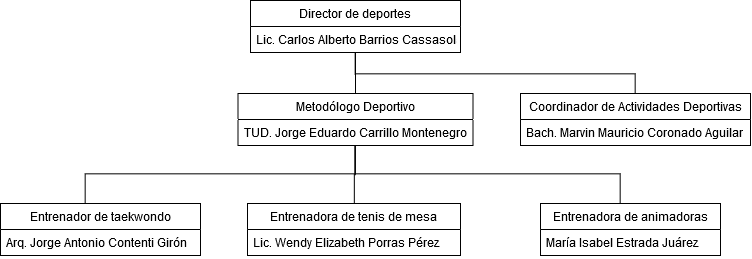
\includegraphics[width=450px,height=170px]{graphics/orgDeportes.png} \\
	\textbf{Fuente:} Propia.
\end{figure}
\subsection{Unidades de an\'alisis} \label{sj:ua}
Para el presente proyecto se utiliz\'o como referencia el manual de acondicionamiento de fuerza y prevenci\'on de lesiones  \cite{arbour2006strength}, la cual describe los movimientos ideales para el calentamiento  y estiramiento de una rutina. (Ver secci\'on de anexos \ref{anx:warmup}).
\section{Instrumentos}\label{ins}
El conjunto de instrumentos se elabor\'o con los  siguientes recursos:
\begin{itemize}
\item Humanos
	\begin{itemize}
	\item Profesionales (entrenadores deportivos).
	\item Atletas
	\item Investigador
	\end{itemize}
\item No humanos
	\begin{itemize}
	\item Mesa de soporte con una altura de 0.70 metros.
	\item Cable de extensi\'on el\'ectrico de 2.00 metros. 
	\item Computadora port\'atil
		\begin{itemize}
		\item Conector de carga de alimentaci\'on
		\end{itemize}
	\item Sensor Kinect
		\begin{itemize}
		\item Adaptador del Kinect
		\end{itemize}
	\end{itemize}
\end{itemize}
\subsection{Formulario de registro de movimiento} \label{ins:frmMov}
Este formulario se adjunta en anexos (ver figura \ref{fig:frmWhiteMov}), la cual tiene como objetivo describir el movimiento v\'alido de cada equipo deportivo. Por otra parte, el formulario est\'a compuesto por los siguientes incisos:
\begin{itemize}
	\item \textbf{Nombre del movimiento:} Nombre que se identifica en gu\'ias deportivas o de salud.
	\item \textbf{Descripci\'on del movimiento: } Contesta la pregunta: ?`Qu\'e es el movimiento?
	\item \textbf{Movimiento unilateral:} Si es afirmativo, el movimiento trabaja con solo una parte del cuerpo (izquierda o derecha, ejemplo una patada), en caso contrario, se considera todas las partes del cuerpo (izquierda y derecha, ejemplo un salto).
	\item \textbf{Partes del cuerpo ignorada:} M\'ultiples respuestas que identifican las articulaciones ignoradas (debido que no es informaci\'on relevante para el movimiento):
	\begin{itemize}
		\item \textbf{Brazo derecho o izquierdo:} Ignora las siguientes articulaciones (seg\'un su lado): Pulgar, dedo del medio, mano, codo, hombro, centro de los hombros, cuello, cabeza y espalda.
		\item \textbf{Cuerpo inferior:} Ignora las siguientes articulaciones (en ambos lados): Centro de cadera, caderas, rodillas, tobillos y pies.
	\end{itemize}
		\item \textbf{N\'umero de pasos:} Cantidad de pasos del movimiento.
		\item \textbf{Offset del paso:} Valor que separa las etiquetas por partes iguales.
		\item \textbf{Valor de identificaci\'on:} Valor que reconoce las etiquetas por partes iguales.
		\item \textbf{Detalle por paso:} Muestra los pasos establecidos por el profesional, para ejecutar un movimiento v\'alido:
			\begin{itemize}
		\item \textbf{Paso:} N\'umero \'unico que identifica el paso.
		\item \textbf{Diagrama:} Imagen visual del paso (seguimiento del esqueleto).
		\item \textbf{Descripci\'on del paso:} Responde la pregunta: ?`Cu\'al es la postura del cuerpo durante ese paso?
		\item \textbf{Etiqueta:} N\'umero \'unico que identifica el paso a partir de la probabilidad de movimiento.
	\item \textbf{Rango de identificaci\'on:} Rango m\'aximo que identifica el paso dentro de la probabilidad del movimiento.
	\end{itemize}
\end{itemize}
\subsection{Formulario de registro de rutina} \label{ins:frmRout}
Formulario adjuntado en anexos (Ver figura \ref{fig:frmWhiteRout}), tiene como funci\'on identificar los ejercicios de calentamiento  previamente a realizar el movimiento seleccionado por cada equipo deportivo, adem\'as de estandarizar el n\'umero de repeticiones del movimiento por cada atleta, a partir de los siguientes puntos:
\begin{itemize}
	\item \textbf{Descripci\'on del calentamiento:} Detalla el tipo de calentamiento (calentamiento con tu propio peso, calentamiento dentro de un ambiente, calentamiento a partir de objetos).
	\item \textbf{Movimientos:} Lista los movimientos que se realizan durante el calentamiento (Validado por el formulario de registro de movimiento).
	\item \textbf{Series:} Cantidad de veces que debe realizar un atleta, un conjunto de repeticiones del movimiento.
	\item \textbf{Repeticiones:} Cantidad de repeticiones del movimiento.
	\item \textbf{Tiempo:} Duraci\'on del calentamiento.
	\item \textbf{Im\'agenes:} Fotograf\'ias tomadas durante el entrenamiento de cada equipo deportivo.
	\item \textbf{Nombre del movimiento:} Movimiento seleccionado por cada equipo deportivo  (validado por el formulario de registro de movimiento).
	\item \textbf{Rutina:} Describe el tipo de rutina para la captura de datos:
	\begin{itemize}
		\item \textbf{Por tiempo:} M\'axima cantidad de repeticiones del movimiento, durante un tiempo establecido.
		\item \textbf{Escaleras:} N\'umeros de repeticiones establecidas, separadas por series.
	\end{itemize}	
\end{itemize}
\subsection{Interfaces de usuarios} \label{ins:UI}
Aplicaciones que interact\'uan con el usuario para la recolecci\'on de datos, en donde se trabajan con  tres tipos:
\subsubsection{Windows presentation foundation (WPF)}
\label{ins:UI:wpf}
El desarrollador, \citeA{wpf2019}, menciona que este tipo de interfaz permite crear aplicaciones de escritorio con la tecnolog\'ia .NET, la cual es soportado desde Windows XP hasta la \'ultima versi\'on de Windows (Windows 10). Por lo tanto, en el presente proyecto se utiliz\'o este tipo de interfaz para la construcci\'on del seguimiento del esqueleto, generado por los siguientes kits de desarrollo de software:
\begin{itemize}
	\item \textbf{Windows inputs:} Herramienta que permite crear elementos de un formulario (e.g. botones, cajas de textos) \cite{wpfWindows2019}.
	\item \textbf{Windows media:} Herramientas que permiten renderizar el seguimiento del esqueleto en tiempo real a partir de pinceles, colores, formas y dibujos \cite{WindowMedia2019}.
	\item \textbf{Windows threading:} Herramientas que permiten crear temporizadores para la renderizaci\'on del seguimiento del esqueleto en un per\'iodo del tiempo (30 fotogramas por segundos) \cite{WindowThreading2019}.
	\item \textbf{Kinect:} Herramientas que permiten acceder a las funcionalidades del sensor \cite{WindowKinect2019}, tales:
	\begin{itemize}
					\item \textbf{Body frame reader:} Obtiene la informaci\'on del seguimiento del esqueleto.
				\item \textbf{Estado del sensor:} Activo, pausa, no detectado e inactivo.
				\item \textbf{Datos del Visual Gesture Builder:} Normalizaci\'on de datos del sensor del Kinect para el uso del modelo de reconocimiento de movimiento.
			\item \textbf{Joint type:} Enumeradores que listan las articulaciones del seguimiento del esqueleto (e.g. manos, codos, hombros).
			\item \textbf{Visualizaci\'on de los recursos de los fotogramas para Visual Gesture Builder:} Interpreta la base de datos de gesturas y posiciones de un movimiento (.gdb), a partir del algoritmo Random Forest Regression.
	\end{itemize}	 
\end{itemize}
A partir de los kits de desarrollo se crearon 2 aplicaciones para la captura de informaci\'on.
\paragraph{Detecci\'on de profundidad}\mbox{} \\ \label{ins:UI:wpf:depth}
Esta aplicaci\'on tiene como objetivo recolectar la distancia correcta de profundidad entre el atleta y el Kinect, tomando en cuenta una articulaci\'on de an\'alisis, adem\'as de la altura del usuario medida desde la cabeza hasta los pies, tal como se presenta en la imagen de la interfaz gr\'afica de detecci\'on de profundidad:
\begin{figure}[H]
	\caption{Interfaz gr\'afica de detecci\'on de profundidad entre el usuario y el sensor}
	\label{fig:appDepth}
	\centering
	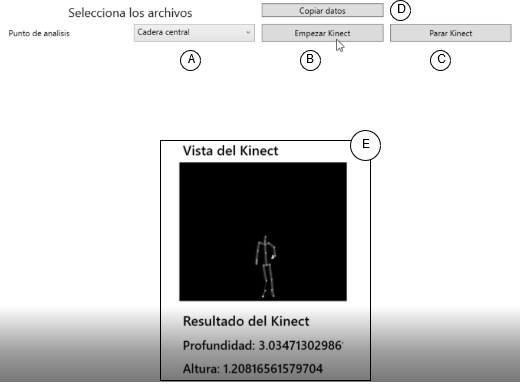
\includegraphics[width=380px,height=200px]{graphics/appProfundidad.png} \\
	\textbf{Fuente:} Propia.
\end{figure}
Esta interfaz se compone por 5 componentes:
\begin{enumerate}[A.]
    \item Selecci\'on de una articulaci\'on de an\'alisis.
    \item Bot\'on que empieza las funcionalidades del seguimiento del esqueleto.
    \item Bot\'on que finaliza las funcionalidades del seguimiento del esqueleto.
    \item Conjunto de paneles de controles que muestran una imagen en tiempo real del seguimiento del esqueleto, adem\'as de la altura (en metros) del usuario y la distancia de profundidad (en metros) entre el atleta y el sensor.
        \item Bot\'on que permite copiar a una hoja de observaci\'on (ver anexos, cuadro \ref{tab:obsDepth}) los siguientes datos respectivos: N\'umero de identificaci\'on de la articulaci\'on, la distancia de profundidad y la altura del usuario.
\end{enumerate}
\paragraph{Evaluaci\'on del movimiento}\mbox{} \\\label{ins:UI:wpf:evaluate}
Aplicaci\'on realizada por el autor del usuario, cuya funcionalidad es programar una rutina de tabata a partir del movimiento de cada equipo deportivo, mostrado en la interfaz gr\'afica de evaluaci\'on de un movimiento:
\begin{figure}[H]
	\caption{Interfaz gr\'afica de evaluaci\'on de un movimiento}
	\label{fig:appEvaluate}
	\centering
	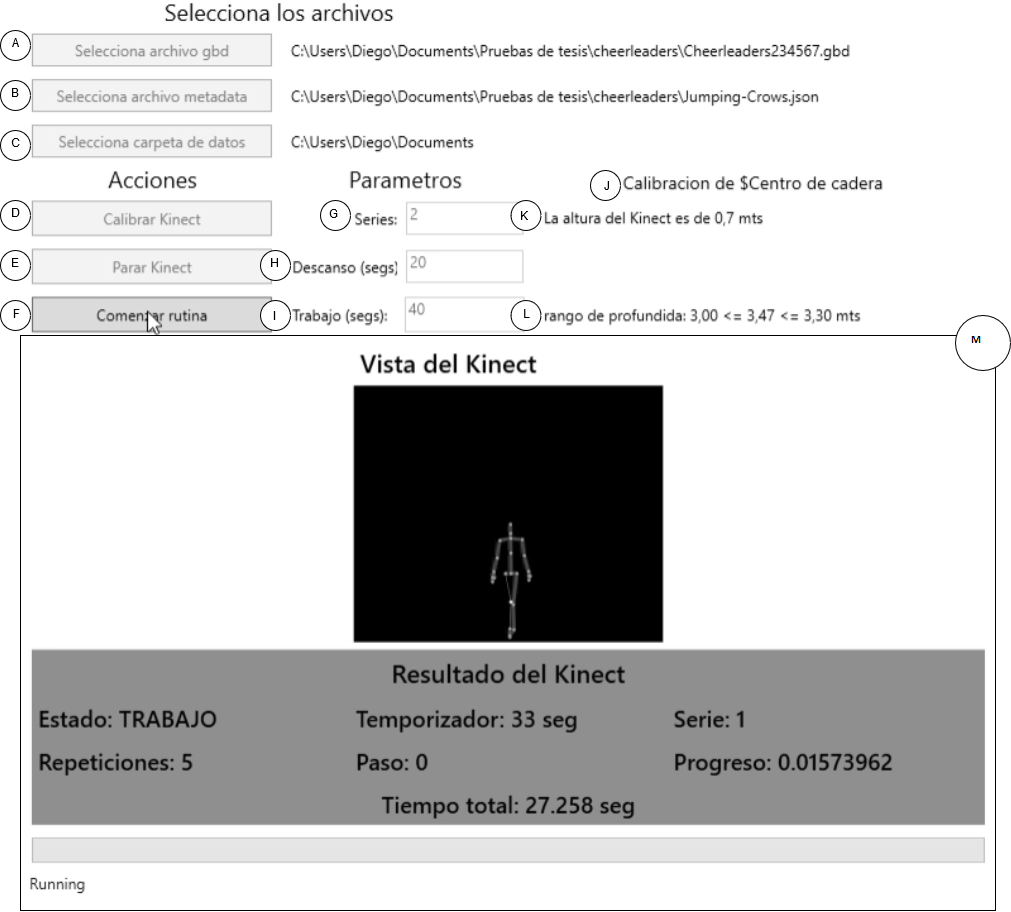
\includegraphics[width=380px,height=250px]{graphics/appEvaluacion.png} \\
	\textbf{Fuente:} Propia.
\end{figure}
Dicha interfaz se divide en 13 componentes:
\begin{enumerate}[A.]
    \item Bot\'on que permite seleccionar el archivo de base de datos del reconocimiento del movimiento.
    \item Bot\'on que permite seleccionar el archivo json que contiene toda la informaci\'on respectiva del movimiento (ver anexos, c\'odigo  \ref{code:jsonMeta}).
    \item Bot\'on que permite seleccionar la direcci\'on del archivo de resultado de tabata.
    \item Bot\'on que permite activar todas las funcionalidades del Kinect.    
    \item Bot\'on que permite detener todas las funcionalidades del Kinect. 
    \item Bot\'on que permite comenzar la rutina de tabata (en tiempo real).
   \item  Caja de texto num\'erica que indica la cantidad de tiempos de trabajos y descansos del atleta durante su rutina de tabata.
   \item  Caja de texto num\'erica que se\~nala el tiempo de descanso durante una rutina.
   \item  Caja de texto n\'umerica que muestra el tiempo de trabajo durante una rutina (durante este tiempo, el atleta debe realizar la cantidad m\'axima de repeticiones).
   \item  Etiqueta de articulaci\'on de an\'alisis para medir la distancia de profundidad entre el atleta y el sensor.
   \item  Etiqueta de la altura  recomendada (en metros)  del sensor y el suelo.
      \item  Etiqueta de la distancia m\'inima y m\'axima de profundidad del atleta con respecto al sensor, y por otra parte indica la distancia profundidad actual del usuario y el sensor.
      \item Conjunto de paneles de controles que muestran:
      \begin{itemize}
            \item  El seguimiento del esqueleto en tiempo real.
            \item  Estado actual de la rutina: Inicio, trabajo, descanso y fin.
            \item  Temporizador de cuenta regresiva del tiempo de trabajo o descanso (en segundos).
             \item  Serie actual que est\'a trabajando el atleta.
             \item  Contador de repeticiones de la serie actual.
              \item \'Ultimo paso ejecutado por el atleta (comenzando desde 0).   
             \item  Valor de probabilidad del movimiento (factor del movimiento).
             \item  Temporizador que mide el tiempo    empleado en la rutina (en segundos).
      \end{itemize}
\end{enumerate}
Ya definido los componentes de la interfaz, se debe tomar en cuenta que al finalizar cada rutina tabata  el programa genera un archivo json (ver anexos, c\'odigo  \ref{code:tabata}), con los siguientes resultados:
\begin{itemize}
	\item \textbf{Analizador de variables:} Indica las variables que fueron configurado en un tabata: Tiempo de descanso, tiempo de trabajo y la cantidad de series.
	\item  \textbf{Resultados generales:} Muestran los resultados del volumen de repeticiones  y el tiempo total empleado en la rutina de tabata.
	\item  \textbf{Resistencia:} Vector de informaci\'on que permite construir la gr\'afica de la rutina tabata, a partir de los siguientes par\'ametros:
	   \begin{itemize}  
   	\item \textbf{Uid:} C\'odigo \'unico de identificaci\'on de la gr\'afica.
   	\item \textbf{Label:} Nombre de la gr\'afica.
   	\item \textbf{Show line:} Condici\'on que permite dibujar la l\'inea de la tendencia de la gr\'afica.
    \item \textbf{Data:} Vector de datos que conforma la gr\'afica, en donde los datos del eje x, representan el tiempo de rutina (en segundos), y los datos del eje y, significan las repeticiones acumulada durante ese tiempo de rutina.
   \end{itemize}     
    \item \textbf{Potencia:} Cantidad de repeticiones m\'axima del movimiento, en el menor tiempo posible.
    \item \textbf{Velocidad:} Se divide en dos resultados:
           \begin{itemize}
       \item Cantidad promedio de repeticiones en una serie.
       \item Tiempo promedio por una repetici\'on
       \end{itemize}
\end{itemize} 
\subsubsection{Web}\mbox{} \\
\label{ins:UI:web}
Interfaz de usuario que permite capturar la informaci\'on de los formularios de movimiento, a partir de la siguiente arquitectura:
\begin{figure}[H]
	\caption{Arquitectura web}
	\label{fig:architectureWeb}
	\centering
	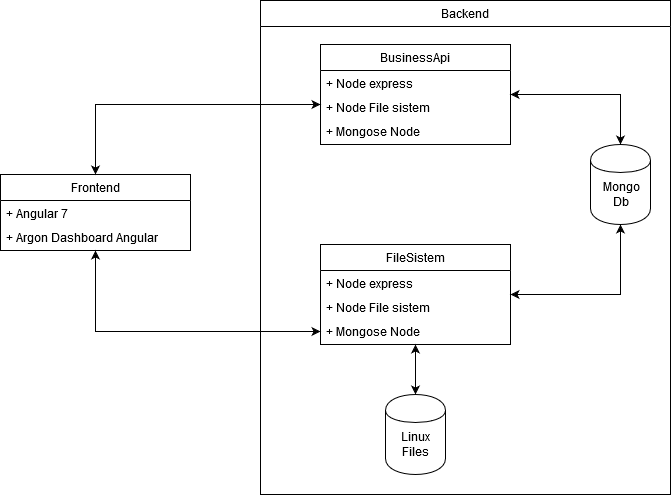
\includegraphics[width=430px,height=220px]{graphics/webArchitecture.PNG} \\
	\textbf{Fuente:} Propia.
\end{figure}
\begin{itemize}
\item Frontend
	\begin{itemize}
	\item \textbf{Web}: Interfaz agradable para el usuario, cuya finalidad es realizar llamadas a las aplicaciones de negocio y servidor de archivos.
	\end{itemize}
\item Backend
	\begin{itemize}
	\item \textbf{Business api:} Maneja todas las  funciones l\'ogicas del giro de negocios (e.g. Insertar movimiento, leer movimiento, resultados de rutina).
	\item \textbf{File sistem:} Interfaz de programaci\'on de aplicaciones que se encarga de almacenar los archivos de metadata que define una base de datos del movimiento.
		\item \textbf{Server files:} Servidor encargado de almacenar los archivos de bases de datos del movimiento v\'alido (.gdb) y sus respectivos v\'ideos (.xef).
		\item \textbf{Mongo DB:} Servidor de bases de datos no relacional, que se encarga de almacenar informaci\'on de la metadata del movimiento.
	\end{itemize}
\item Entornos de trabajo
\begin{itemize}
\item \textbf{Angular 7:} Herramienta que facilita la creaci\'on y el mantenimiento de una aplicaci\'on web \cite{angular2019}.
\item \textbf{Argon dashboard angular:} Herramienta  que facilita realizar una aplicaci\'on responsiva (adaptable a cualquier dispositivo a partir de un navegador web) \cite{argonDash}.
\item \textbf{Express js:} Herramienta encargada de realizar la comunicaci\'on entre aplicaciones, a partir del \acrlong{HTTP} \cite{fileSistem2019}.
\item \textbf{Mongoose:} Herramienta encargada de realizar cualquier operaci\'on de la base de datos de mongo (e.g. conexi\'on, recuperar datos, modificar registros) \cite{mongoose2019}.
\end{itemize}
\end{itemize}
As\'i mismo la aplicaci\'on web est\'a conformada por 4 vistas:
\paragraph{Vista del listado de movimientos}\mbox{} \\ \label{ins:UI:web:index}
Vista principal que muestra al usuario todos los movimientos que se han insertado en la base de datos.
\begin{figure}[H]
	\caption{Vista de listado de movimientos}
	\label{fig:viewIndex}
	\centering
	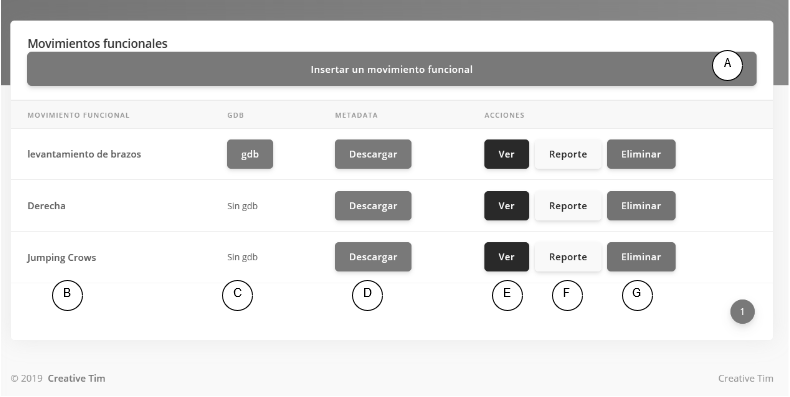
\includegraphics[width=440px,height=270px]{graphics/web-index.PNG} \\
	\textbf{Fuente:} Propia.
\end{figure}
\begin{enumerate}[A.]
\item Bot\'on que dirige al usuario a la pantalla de insertar un movimiento (Ver vista de creaci\'on de un movimiento).
\item Etiqueta que indica el nombre del movimiento.
\item Bot\'on que descarga el archivo de base de datos de un movimiento.
\item Bot\'on que exporta el archivo de metadata de un movimiento (Ver anexos, c\'odigo \ref{code:jsonMeta}), con los siguientes atributos:
	\begin{itemize}
	\item \textbf{Steps}: Vector num\'erico que contiene las etiquetas de cada paso de un movimiento.
	\item \textbf{Angles of movement}: Vector num\'erico que almacena los \'indices de cada articulaci\'on que interact\'uan en el movimiento.
	\item \textbf{Recognition}: Valor que construye  el rango de confiabilidad para detectar un paso de un movimiento.
	\item \textbf{Id}: C\'odigo \'unico que identifica el movimiento en la base de datos.
	\item \textbf{Height}: Altura del Kinect con respecto al suelo (medida en metros).	
	\item \textbf{Depth min}: Distancia m\'inima de profundidad del sensor y el atleta (medida en metros).
	\item \textbf{Depth max}: Distancia m\'axima de profundidad del sensor y el atleta (medida en metros).
	\item \textbf{Time stamp}: Fecha en la cual fue insertado el registro del movimiento.
	\item \textbf{Focus join}: Articulaci\'on de an\'alisis que permite medir la distancia de profundidad. 
	\end{itemize}
\item Bot\'on que dirige al usuario a la pantalla de detalle de un movimiento (ver vista de lectura de un movimiento).
\item Bot\'on que dirige al usuario a la pantalla de reporte de un movimiento (ver vista de resultados de un movimiento).
\item Bot\'on que elimina el registro del movimiento de la base de datos.
\end{enumerate}
\paragraph{Vista de creaci\'on de un movimiento}\mbox{} \\ \label{ins:UI:web:create}
Vista que se encarga de insertar toda la informaci\'on del movimiento, recuperada por los formularios.
\begin{figure}[H]
	\caption{Vista de crear un movimiento}
	\label{fig:viewCreate}
	\centering
	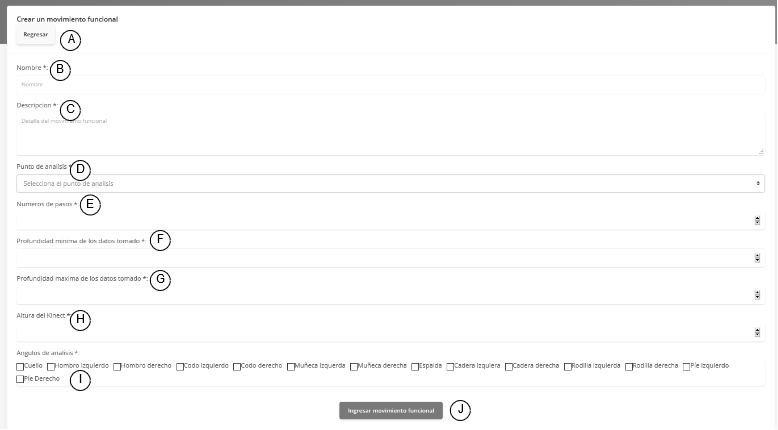
\includegraphics[width=460px,height=320px]{graphics/web-create.PNG} \\
	\textbf{Fuente:} Propia.
\end{figure}
\begin{enumerate}[A.]
\item Bot\'on que dirige al usuario a la pantalla del listado de los movimientos (ver vista de listado de movimientos).
\item Caja de texto para ingresar el nombre del movimiento (Recuperado del formulario de registro de movimiento, atributo de nombre).
\item Caja de texto para ingresar el detalle del movimiento (Recuperado del formulario de registro de movimiento, atributo de descripci\'on).
\item Selecci\'on de la articulaci\'on de an\'alisis (recuperado de la aplicaci\'on de detecci\'on de profundidad, atributo de articulaci\'on de an\'alisis).
\item Caja de texto num\'erica que ingresa la cantidad de pasos del movimiento (recuperado del formulario de registro de movimiento, atributo de n\'umero de pasos).
\item Caja de texto num\'erica que ingresa la distancia m\'inima de profundidad (ver formula \ref{frm:maxDepth}).
\item Caja de texto num\'erica que ingresa la distancia m\'axima de profundidad (ver formula \ref{frm:minDepth}).
\item Caja de texto num\'erica que ingresa la altura del Kinect con respecto al suelo (para el presente proyecto es de 0.70 metros, debido que es la altura de la mesa que daba soporte al sensor).
\item Listado m\'ultiples de articulaciones que intervienen en el movimiento (recuperado del formulario de registro de rutinas, atributo de articulaciones no ignoradas).
\item Bot\'on que almacena toda la informaci\'on respectiva del formulario web.
\end{enumerate}
\paragraph{Vista de lectura de un movimiento}\mbox{} \\ \label{ins:UI:web:read}
Vista que se encarga de mostrar toda la informaci\'on del movimiento, adem\'as de insertar el archivo de base de datos de gesturas y modificar el rango de confiabilidad de reconocimiento de pasos.
\begin{figure}[H]
	\caption{Vista de lectura del movimiento}
	\label{fig:viewRead}
	\centering
	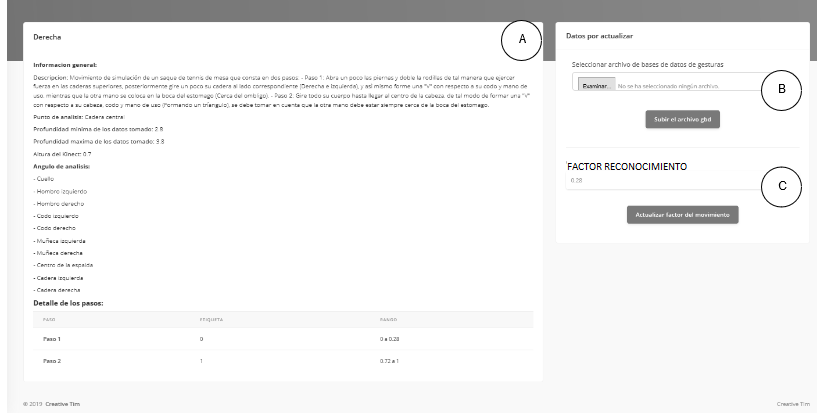
\includegraphics[width=460px,height=320px]{graphics/web-read.PNG} \\
	\textbf{Fuente:} Propia.
\end{figure}
\begin{enumerate}[A.]
\item Ficha de informaci\'on que detalla todas las caracter\'isticas del movimiento (e.g. Nombre, descripci\'on, etiquetas de los pasos, intervalos de confianza de los pasos, articulaciones del movimiento).
\item Conjuntos de controladores que permiten seleccionar un archivo de base de datos de gesturas y almacenarlo en el servidor de archivos.
\item Conjunto de controladores que permiten cambiar el valor del factor de reconocimiento (Ver ecuaci\'on \ref{frm:rangoConfiabilidad}).
\end{enumerate}
\paragraph{Vista de resultados de un movimiento}\mbox{} \\ \label{ins:UI:web:result}
Vista que expone los resultados de la aplicaci\'on de evaluaci\'on de un movimiento:
\begin{figure}[H]
	\caption{Resultados de la rutina tabata de un movimiento}
	\label{fig:resultsTabata}
	\centering
	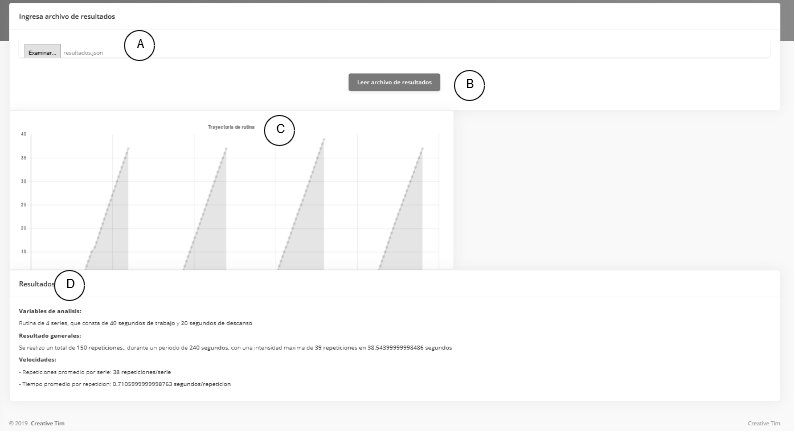
\includegraphics[width=460px,height=320px]{graphics/web-results.PNG} \\
	\textbf{Fuente:} Propia.
\end{figure}
\begin{enumerate}[A.]
\item Conjuntos de controladores que seleccionan y leen un archivo de resultados de la rutina tabata (ver anexos, c\'odigo \ref{code:tabata}).
\item Diagrama de dispersi\'on de la rutina tabata, la cual muestra las repeticiones acumuladas durante tiempos de trabajos y de descansos.
\item Ficha informativa que muestra los resultados de la rutina tabata (e.g. Variables que fueron configuradas en el tabata, volumen de repeticiones, duraci\'on de la rutina, repeticiones por serie de trabajo, tiempo promedio por repetici\'on).
\end{enumerate}
\subsubsection{Consola (Windows)}\mbox{} \\ \label{ins:cons}
\begin{figure}[H]
	\caption{Aplicaci\'on de extracci\'on de datos en los v\'ideos (xef)}
	\label{fig:appConsole}
	\centering
	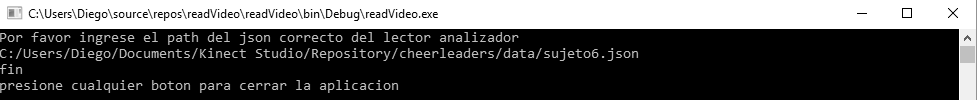
\includegraphics[width=460px,height=50px]{graphics/appConsole.PNG} \\
	\textbf{Fuente:} Propia.
\end{figure} 
Aplicaci\'on de consola que permite extraer informaci\'on de los v\'ideos (.xef) y generar una hoja de observaciones del seguimiento de esqueleto (ver anexo, tabla \ref{tab:obsVideoData}), con la ayuda de las siguientes herramientas:
\begin{itemize}
\item \textbf{System console:} Permite utilizar todas las funcionalidades de consola de windows \cite{windowConsole2019}.
\item \textbf{System io:} Proporciona todas las  funcionalidades de manejo de archivos \cite{windowIO2019}.
\item \textbf{Kinect xef tools:} Librer\'ia que extrae de los v\'ideos (xef), la posici\'on de cada articulaci\'on del seguimiento del tiempo, durante un per\'iodo del tiempo \cite{kinectXEFTools}.
\end{itemize}
Para el funcionamiento de la aplicaci\'on, es necesario un archivo de lector analizador (ver anexos, c\'odigo \ref{code:jsonVideo}), en donde est\'a conformado por los siguientes atributos:
\begin{itemize}
\item \textbf{Path video:} Direcci\'on del archivo  de v\'ideo a analizar (.xef).
\item \textbf{Path write:} Direcci\'on del archivo  resultante (.csv).
\item \textbf{Joints:} Vector num\'erico que muestra los \'indices de las articulaciones que se desean extraer la informaci\'on.
\item \textbf{Frame data:} Vector de vectores de cadenas, la cual por cada vector de cadena se indica el segmento de v\'ideo de extracci\'on de datos (punto de inicio y punto final).
\end{itemize}
\subsection{Kinect configuration verifier} \label{ins:KinectCheckt}
Herramienta del kit de desarrollo de software del sensor del Kinect, que tiene como objetivo  analizar la computadora que se encuentra conectado al sensor, verificando las compatibilidades del hardware (e.g. procesador, controlador de usb, sistema operativo, conexi\'on del sensor), adem\'as de chequear la comunicaci\'on con la c\'amara (e.g. canales de color y de profundidad).
\subsection{Kinect studio} \label{ins:KinectStudio}
Herramienta del kit de desarrollo de software del sensor del Kinect que se utiliza para monitorear, grabar (V\'ideos .xef) y reproducir datos de la c\'amara \cite{KinectStudio2019}, a partir de los siguientes canales:
\begin{figure}[H]
	\caption{Canales por defecto para grabar un v\'ideo en Kinect studio }
	\label{fig:streamDefault}
	\centering
	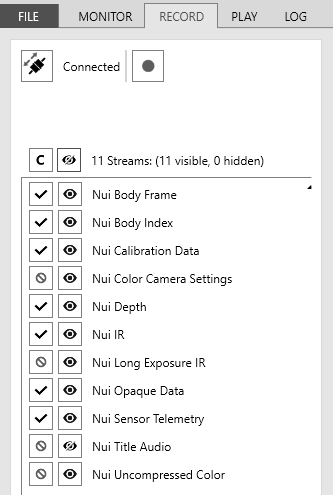
\includegraphics[width=200px,height=360px]{graphics/streamsRecord.PNG} \\
	\textbf{Fuente:} Propia.
\end{figure} 
\begin{itemize}
\item Activos:
\begin{itemize}
\item \textbf{NUI body frame:} Encargado de los datos con relaci\'on al seguimiento del esqueleto.
\item \textbf{NUI body Index:} Identifica de 1 a 6 esqueletos con su respectivo \'indice.
\item \textbf{NUI calibration data:} Responsable de obtener la mayor precisi\'on de datos.
\item \textbf{NUI depth:} Controla y obtiene los datos de profundidad.
\item \textbf{NUI ir:} Monitoreo de los sensores de profundidad.
\item \textbf{NUI opaque data:} Disminuye el ruido de la luz.
\item \textbf{NUI sensor telemetry:} Encargado de actualizar y obtener nuevos datos en un per\'iodo de tiempo.
\end{itemize}
\item Inactivos:
\begin{itemize}
\item \textbf{NUI color camera settings:} Encargado de la conversi\'on de colores (e.g. YUV o RGB)
\item \textbf{NUI long exposure ir:} Identifica  objetos externos al seguimiento del esqueleto (e.g. mesa, pelota, pesa).
\item \textbf{NUI uncompressed color:} Responsable de obtener los datos de color (e.g. c\'odigo de colores de un sem\'aforo).
\end{itemize}
\end{itemize}
As\'i mismo esta herramienta proporciona una interfaz gr\'afica para ver y analizar los v\'ideos a partir de segmentos (parte de inicio y fin) y puntos de pausas.
\begin{figure}[H]
	\caption{Lectura de v\'ideo .xef }
	\label{fig:readVideoXEF}
	\centering
	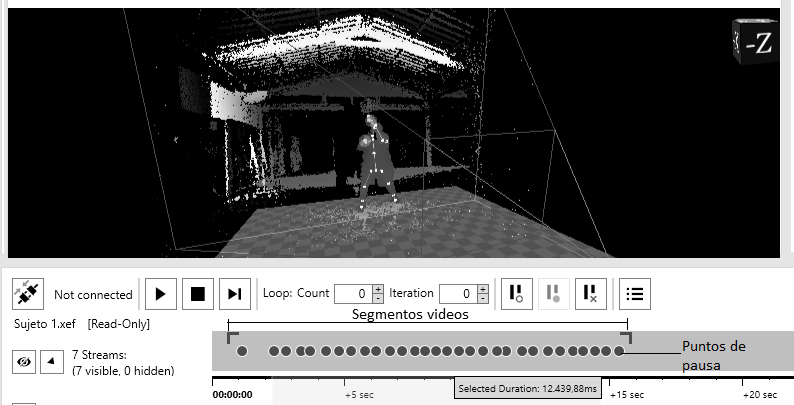
\includegraphics[width=460px,height=320px]{graphics/readVideo.PNG} \\
	\textbf{Fuente:} Propia.
\end{figure} 
\subsection{Visual Gesture Builder} \label{ins:VisualGestureBuilder}
Herramienta que genera datos para la detecci\'on de gestos en tiempo de ejecuci\'on, usando tecnolog\'ias de m\'aquinas de aprendizaje (Random Forest Regression), con el fin objetivo de reconocer un gesto (e.g. saltar, bailar, sentarse) \cite{KinectBuilder2019}, a trav\'es de la etiquetaci\'on de fotogramas y la configuraci\'on de las siguientes variables:
 \begin{figure}[H]
	\caption{Variables de configuraci\'on de Visual Gesture Builder}
	\label{fig:visualGesture}
	\centering
	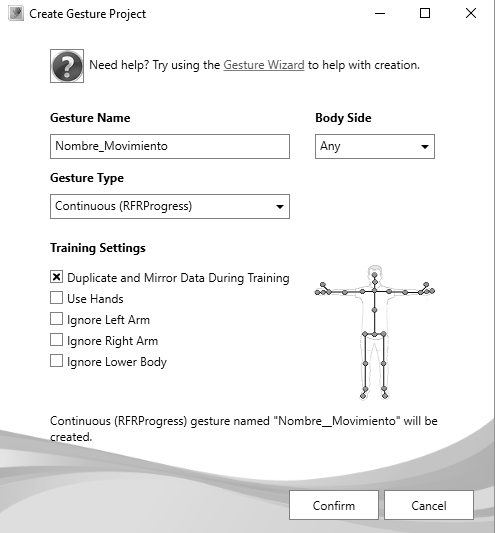
\includegraphics[width=300px,height=300px]{graphics/settingsGesture.PNG} \\
	\textbf{Fuente:} Propia.
\end{figure} 
\begin{itemize}
\item \textbf{Gesture name:} Nombre del movimiento  (Recuperado del formulario de registro de movimiento, atributo de nombre).
\item \textbf{Body side:} Valor por defecto es  ninguno, debido que no importa el lado que se est\'a ejecutando el movimiento, en caso que sea un movimiento unilateral, el modelo replica un modelo espejo, por ejemplo una patada lateral derecha es la replica de una patada lateral izquierda.
\item \textbf{Gesture type:} El valor por defecto es RFRProgress (Algoritmo de Random Forest Regression), debido que est\'a analizando movimiento continuos (e.g. salto, patada, saque).
\item \textbf{Duplicate and mirror data during training:} Se selecciona, si no es un \gls{MovUni} (Ver formulario de registro de movimiento, atributo unilateral), debido que replica datos de lado izquierdo al lado derecho y viceversa, por ejemplo en un salto.
\item \textbf{User hand:} El valor de defecto es falso, debido que no se est\'a analizando el agarre de la mano ante un objeto (e.g. bal\'on, pesa, raqueta).
\item \textbf{Ignore part body:} Se activan  aquellas partes del cuerpo que se desean ignorar durante el movimiento (Ver formulario de registro de movimiento, articulaciones ignoradas).
\end{itemize}
Luego de configurar las variables globales, el proyecto crear\'a una base de datos de gesturas vac\'io, la cual debe adjuntar todos los v\'ideos (.xef)  y por cada v\'ideo se debe etiquetar los valores de fotogramas (Seg\'un los pasos definido en el formulario de registro de movimiento), con el fin objetivo de: 
\begin{itemize}
\item \textbf{Construir:} Acci\'on que entrena y genera el modelo a partir de un archivo de base de datos de gesturas (.gbd).
\item \textbf{Analizar:} Funci\'on que permite seleccionar archivos de base de datos de gesturas y posteriormente compararlo con v\'ideos previamente etiquetados, encontrando el valor real (valor de la etiqueta) y el valor pron\'osticado del modelo (estos valores son usado para completar la hoja de observaci\'on de errores modelo, ver anexos, tabla \ref{tab:obsErrores}).
\end{itemize}
\subsection{Herramienta para el an\'alisis de datos} \label{ins:toolsAn}
Se utiliz\'o el software Microsoft Excel, para la tabulaci\'on y organizaci\'on de los datos.
\section{Procedimiento}
Para el presente proyecto, se implement\'o una metodolog\'ia en cascada con las siguientes  actividades:
\begin{figure}[H]
	\caption{Metodolog\'ia de cascada}
	\label{fig:segVideo}
	\centering
	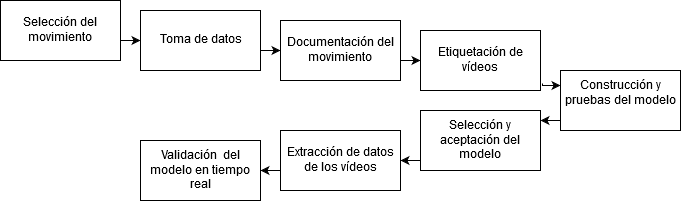
\includegraphics[width=420px,height=80px]{graphics/cascada.PNG} \\
	\textbf{Fuente:} Tomado por el autor de tesis
\end{figure} 
\subsection{Selecci\'on del movimiento}
El investigador visit\'o a cada equipo deportivo durante los d\'ias de entrenamiento -e.g. Lunes de taekwondo, martes de tenis de mesa y mi\'ercoles de animaci\'on-.  Previamente al entrenamiento, el equipo deportivo realizaba series de movimientos que ayudan a calentar y estirar el cuerpo humano.  Luego del calentamiento, el entrenador ense\~naba a los atletas, las t\'ecnicas que ayudan a mejorar el rendimiento deportivo -e.g. Patadas, atrapadas, saques, remates-, y posteriormente cada atleta replicaba los movimientos. Por \'ultimo, el investigador con la ayuda del equipo deportivo, seleccionaron un movimiento de calentamiento -e.g. Jumping jacks, patada lateral y saque derecha-.
\subsection{Toma de datos}
El investigador visit\'o nuevamente a cada equipo deportivo y esper\'o que finalizara la rutina de calentamiento (Durante esa actividad, el investigador instal\'o el prototipo de toma de datos en el lugar asignado), posteriormente al calentamiento, el entrenador seleccionaba a un atleta para participar en la toma de datos (En paralelo, los atletas restantes continuaban con su entrenamiento), el atleta llegaba con el investigador y realizaba dos actividades distintas:
\begin{itemize}
\item La primera actividad constaba en posicionar correctamente al atleta, dicha posici\'on depende de dos condiciones: La primera se chequeaba que se dibuje completamente el seguimiento del esqueleto y la segunda se verificaba que el seguimiento no falle durante la ejecuci\'on del movimiento, lo cual se le solicitaba al atleta realizar 2 repeticiones de prueba. S\'i se cumple ambas condiciones, el investigador apuntaba las observaciones de la altura del usuario y la distancia de profundidad entre el sensor y la cadera central del atleta (capturadas por el instrumento de detecci\'on de profundidad).
\item Al encontrar la posici\'on correctamente, el entrenador le programaba al atleta una rutina en base al movimiento seleccionado (La rutina puede ser dos tipos: Por tiempo o por cantidad de repeticiones), posteriormente se terminaba con la grabaci\'on de la rutina del deportista (grabada por el instrumento Kinect studio).
\end{itemize}
Se debe tomar en cuenta que estas dos actividades se realizaban por cada atleta del equipo deportivo, durante el tiempo de entrenamiento.
 \begin{figure}[H]
	\caption{Fotograf\'ias durante la toma de datos}
	\label{fig:getDataStep}
	\centering
	\includegraphics[width=280px,height=280px]{graphics/tomaDatos.png} \\
	\textbf{Fuente:} Tomado por el autor de tesis
\end{figure} 
\subsection{Documentaci\'on del movimiento}
El investigador realiz\'o una breve entrevista a cada entrenador y algunos atletas (similar a un grupo focal), con la finalidad de detallar todos los aspectos de los movimientos, adem\'as de separar los pasos de cada movimiento. Posteriormente a la entrevista, el investigador complet\'o todos los formularios respectivos de movimiento -i.e. Formularios de datos de entradas-:
\subsubsection{Formularios de entradas de tenis de mesa}
\begin{figure}[H]
	\caption{Formulario de movimiento de tenis de mesa}
	\label{fig:frmMovTen}
	\centering	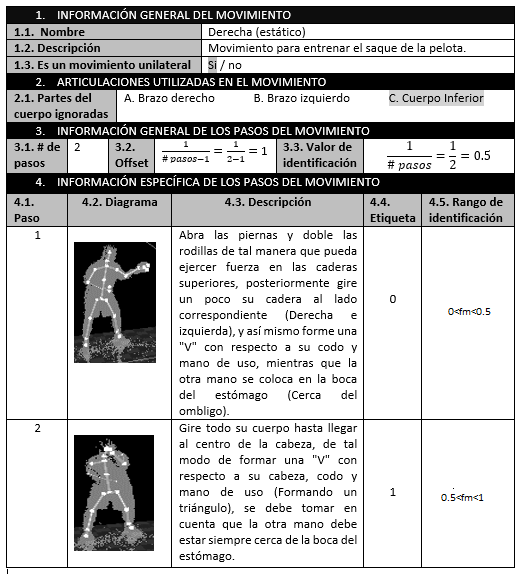
\includegraphics[width=445px,height=600px]{graphics/resultados/movimientoTenis.PNG} \\
	\textbf{Fuente:} Elaborado por el autor de tesis con base a las observaciones del trabajo de campo
\end{figure}
\begin{figure}[H]
	\caption{Formulario de rutina de tenis de mesa}
	\label{fig:frmRoutTen}
	\centering	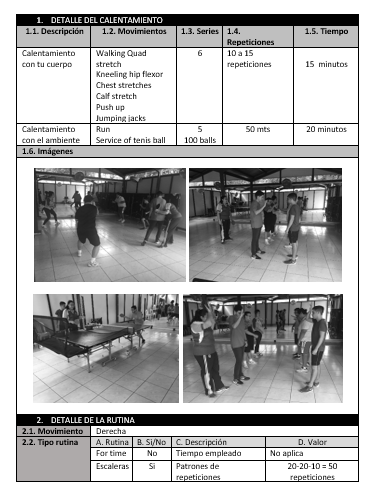
\includegraphics[width=445px,height=600px]{graphics/resultados/rutina-tennis.PNG} \\
	\textbf{Fuente:} Elaborado por el autor de tesis con base a las observaciones del trabajo de campo
\end{figure}
\subsubsection{Formularios de entradas de animaci\'on}
\begin{figure}[H]
	\caption{Formulario de movimiento de animaci\'on}
	\label{fig:frmMovCheer}
	\centering	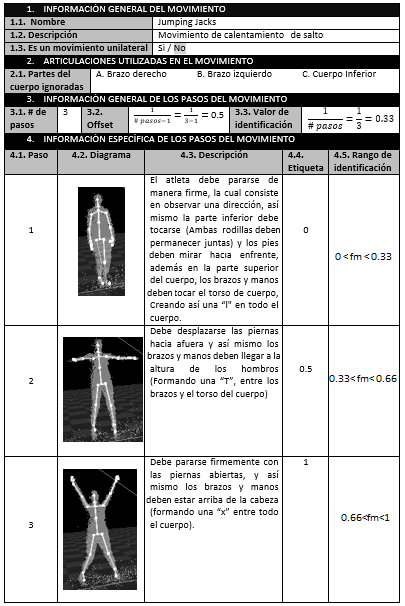
\includegraphics[width=445px,height=600px]{graphics/resultados/movimientoCheerleader.PNG} \\
	\textbf{Fuente:} Elaborado por el autor de tesis con base a las observaciones del trabajo de campo
\end{figure}
\begin{figure}[H]
	\caption{Formulario de rutina de animaci\'on}
	\label{fig:frmRoutCher}
	\centering	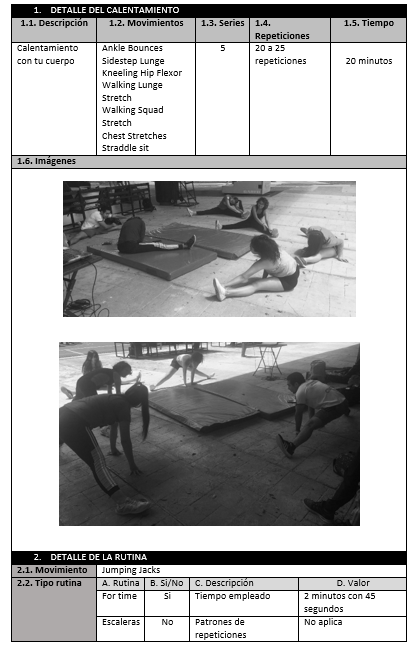
\includegraphics[width=400px,height=490px]{graphics/resultados/rutina-cheerleaders.PNG} \\
	\textbf{Fuente:} Elaborado por el autor de tesis con base a las observaciones del trabajo de campo
\end{figure}
\subsubsection{Formularios de entradas de taekwondo}
\begin{figure}[H]
	\caption{Formulario de movimiento taekwondo}
	\label{fig:frmWhiteMov}
	\centering	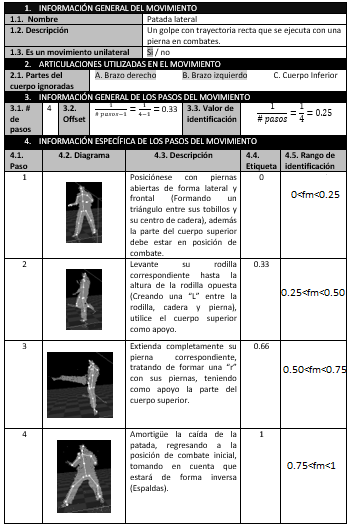
\includegraphics[width=445px,height=600px]{graphics/resultados/movimientoTaekwondo.PNG} \\
	\textbf{Fuente:} Elaborado por el autor de tesis con base a las observaciones del trabajo de campo
\end{figure}
\begin{figure}[H]
	\caption{Formulario de rutina de taekwondo}
	\label{fig:frmRoutTaek}
	\centering	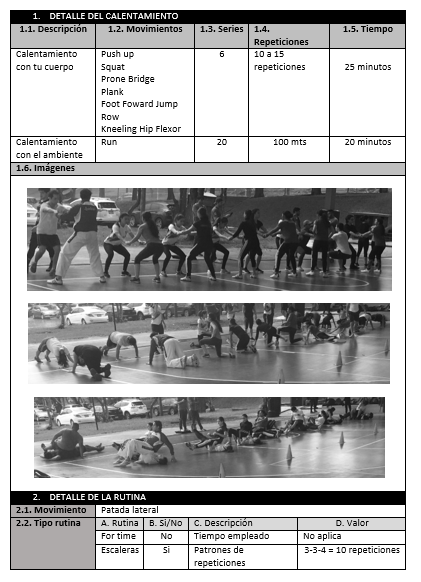
\includegraphics[width=445px,height=600px]{graphics/resultados/rutina-taekwondo.PNG} \\
	\textbf{Fuente:} Elaborado por el autor de tesis con base a las observaciones del trabajo de campo
\end{figure}
\subsection{Etiquetaci\'on de v\'ideos}
El investigador cre\'o desde cero, una base de datos de gesturas por movimiento (a partir del instrumento Visual Gesture Builder), luego se adjunt\'o a la base de datos, todos los v\'ideos recuperados de la actividad de la toma de datos, y por cada v\'ideo se analiz\'o fotograma por fotograma, asignando un valor a cada paso del movimiento, tal como se muestra en figura de proceso de etiquetaci\'on del movimiento:
 \begin{figure}[H]
	\caption{Proceso de etiquetaci\'on del movimiento derecha}
	\label{fig:getTag}
	\centering
	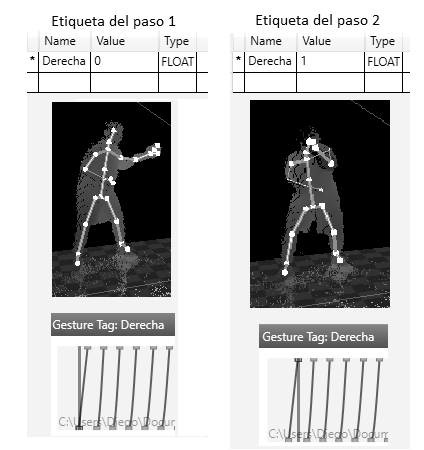
\includegraphics[width=250px,height=250px]{graphics/etiquetas.png} \\
	\textbf{Fuente:} Tomado por el autor de tesis
\end{figure} 
\subsection{Construcci\'on y pruebas del modelo}
Por cada modelo, el investigador separ\'o los v\'ideos etiquetados en dos partes:
\begin{itemize}
\item \textbf{V\'ideos para el entrenamiento y construcci\'on del modelo:} Elementos que permiten  entrenar el modelo, generando un archivo de base de datos de gesturas (.gdb), la cual proporciona el valor del factor de movimiento.
\item \textbf{V\'ideos para an\'alisis:} El investigador seleccion\'o el archivo de bases de datos de gesturas, y posteriormente la herramienta analiz\'o cada v\'ideo, proporcionando el valor real y pronosticado del modelo, tal como se muestra en la figura de obtenci\'on de valores, el valor real es de 0.008018661, mientras que el valor pronosticado es de \num{103893e-6}:
\end{itemize}
 \begin{figure}[H]
	\caption{Obtenci\'on del valor real y pronosticado}
	\label{fig:getError}
	\centering
	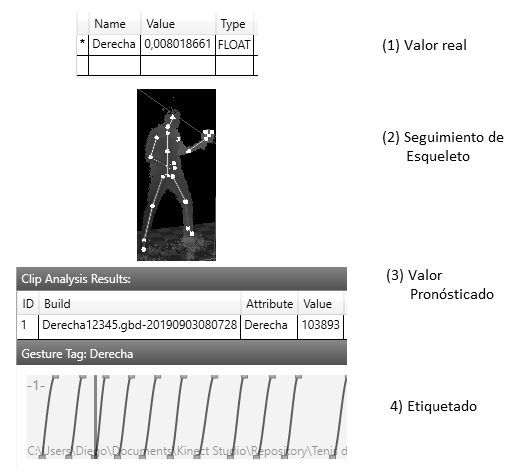
\includegraphics[width=300px,height=300px]{graphics/getError.png} \\
	\textbf{Fuente:} Tomado por el autor de tesis
\end{figure} 
\subsection{Selecci\'on y aceptaci\'on del modelo}
\begin{itemize}
\item \textbf{Selecci\'on:} El investigador realiz\'o tres submodelos distintos por movimiento, con distintos datos de entrenamiento -i.e. Combinaciones de v\'ideos de entrenamientos y an\'alisis-. As\'i mismo por cada submodelo se analiz\'o un v\'ideo de an\'alisis, tabulando los datos reales y pronosticado en una hoja de observaciones (Ver anexos, tabla \ref{tab:obsErrores}). Posteriormente al proceso de tabulaci\'on, se calcul\'o los errores correspondientes de cada modelo -i.e. Error medio pronosticado, desviaci\'on media absoluta y la ra\'iz del error cuadr\'atico medio-, seleccionando as\'i el modelo que tenga un menor error. 
\item \textbf{Aceptaci\'on:} El investigador  verifica la media de los errores de cada submodelo, en caso que el error sea mayor o igual  al valor de reconocimiento (Valor recuperado por los formularios del paso de documentaci\'on del movimiento) se rechaza el modelo, en caso contrario, se da la aprobaci\'on.
\end{itemize}
\subsection{Extracci\'on de datos de los v\'ideos}
Por cada modelo aceptado, el investigador extrajo los datos del tiempo y el recorrido de la mu\~neca derecha de una repetici\'on, con el fin de objetivo de validar que cada modelo fue entrenado con distintos datos, reflejado en una  regresi\'on de tiempo y recorrido. Lo cual para construir dicha regresi\'on, el investigador separ\'o por cada v\'ideo, los renglones de fotogramas de una repetici\'on, listando los tiempos iniciales y finales utilizado para la extracci\'on de datos de v\'ideos .xef (recuperado del instrumento, Kinect studio).
\begin{figure}[H]
	\caption{Segmentos de repeticiones de un v\'ideo}
	\label{fig:segVideo}
	\centering
	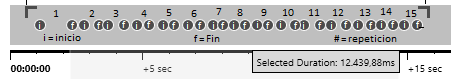
\includegraphics[width=420px,height=100px]{graphics/separarPuntos.PNG} \\
	\textbf{Fuente:} Tomado por el autor de tesis
\end{figure} 
\subsection{Validaci\'on  del modelo en tiempo real}
El investigador realiz\'o una \'ultima visita a cada equipo deportivo (cuyo modelo fue aprobado), en dicha visita instal\'o el prototipo del modelo en lugar asignado (en paralelo, los atletas realizaban el calentamiento), posteriormente a la instalaci\'on, el investigador le ense\~n\'o al entrenador una versi\'on de prueba de una rutina tabata, dicha prueba lo realiz\'o el investigador (Cabe resaltar que el investigador vest\'ia deportivamente y adem\'as ejecut\'o previamente los ejercicios de calentamiento) con una rutina de 1 serie de 10 segundos de descanso y 50 segundos de trabajo. Luego de la prueba, el entrenador seleccion\'o a un grupo de atletas que no participaron en el proceso de toma de datos, y posteriormente se le program\'o a cada atleta del grupo, una rutina tabata (cada deportista se posicion\'o en la distancia de profundidad recomendada).
 \begin{figure}[H]
	\caption{Fotograf\'ias durante la validaci\'on del modelo}
	\label{fig:getvalidationStep}
	\centering
	\includegraphics[width=165px,height=165px]{graphics/tabataResultados.png} \\
	\textbf{Fuente:} Tomado por el autor de tesis
\end{figure} 
\section{Dise\~no de la metodolog\'ia}\label{dis}
Esta secci\'on se presenta todos los dise\~nos y c\'alculos matem\'aticos y estad\'isticos encontrados en los resultados. 
\subsection{Asignaci\'on de valores de etiquetas y rangos de identificaci\'on}\label{dis:asig}
Estos valores permiten identificar el paso de cada movimiento a partir de las siguientes variables:
\begin{itemize}
\item \textbf{Offset:} Valor de distribuci\'on de etiquetas de cada paso del movimiento, por partes iguales.
\begin{formula}[H]
	\centering
	\caption{Offset de etiquetas}
	\label{frm:offsetEt}
	\begin{equation}
offset = \frac{1}{pasos-1}
	\end{equation}
	\textbf{Fuente:} Propia
\end{formula}
\item \textbf{Vector de etiquetas:} A cada paso se le distribuye un valor \'unico, cuyo valor se calcula a partir del offset de la etiqueta anterior.
\begin{formula}[H]
	\centering
	\caption{Asignaci\'on de etiquetas}
	\label{frm:vecEtiq}
	\begin{equation}
\begin{matrix}
etiquetas=[0, etiqueta(1), ..., etiqueta(paso), ..., 1],\; donde
\\
\\
etiqueta(paso) =
\left\{\begin{matrix}
0 & Si\; es\; el\; primer \; paso
\\
etiqueta(paso-1)+offset & Si\; es\; un\; paso\; intermedio
\\ 
1 & Si\; es\; el\; \acute{u}ltimo\; paso
\end{matrix}\right.
\end{matrix}
	\end{equation}
	\textbf{Fuente:} Propia
\end{formula} 

\item \textbf{Valor de identificaci\'on:} N\'umero que representa la distribuci\'on de reconocimiento  de pasos por partes iguales:
\begin{formula}[H]
	\centering
	\caption{Valor de identificaci\'on de pasos}
	\label{frm:idenStep}
	\begin{equation}
valor \: de \: identificaci\acute{o}n = \frac{1}{pasos}
	\end{equation}
	\textbf{Fuente:} Propia
\end{formula} 

\item \textbf{Rango de identificaci\'on:} Rango m\'aximo num\'erico para identificar un paso.
\begin{formula}[H]
	\centering
	\caption{Rango m\'aximo de identificaci\'on de un paso}
	\label{frm:idenStep}
	\begin{equation}
\begin{matrix}
rango = [[inferior,superior]] \\
\\
rango(paso)=\left\{\begin{matrix}
inferior(paso)= \left\{\begin{matrix}
0 & paso\: inicial\\ 
superior(paso-1) & paso\: no\: inicial
\end{matrix}\right.\\ 
\\
superior(paso)= \left\{\begin{matrix}
inferior(paso)+identificaci\acute{o}n & paso\, no\, final\\ 
1 & paso\: final

\end{matrix}\right.\\ 
\end{matrix}\right.
\end{matrix}
	\end{equation}
	\textbf{Fuente:} Propia
\end{formula} 
\end{itemize}
\subsection{C\'alculo indirecto de la altura del usuario} \label{dis:height}
Para el presente proyecto se midi\'o la altura del usuario, a partir de la diferencia entre la altura de la cabeza y la altura promedio de los pies.
	\begin{formula}[H]
	\centering
	\caption{Altura del usuario}
	\label{frm:alturaUser}
	\begin{equation}
y_{usuario}=y_{cabeza}-\frac{y_{pie \: derecho}+y_{pie \: izquierdo}}{2}
	\end{equation}
			\textbf{Fuente:} Planteado por el autor de tesis
\end{formula} 
\subsection{C\'alculo de distancia de profundidad m\'inima y m\'axima} \label{dis:deep}
Para los siguientes c\'alculos se utilizaron la hoja de observaciones de profundidad (Ver anexo, tabla  \ref{tab:obsDepth}), aplicando las siguientes funciones de microsoft excel (versi\'on ingl\'es):
\begin{itemize}
       \item \textbf{Average}: Funci\'on para determinar la altura promedio.
\begin{formula}[H]
	\centering
	\caption{C\'alculo de altura promedio}
	\label{frm:avgHeight}
	\begin{equation}
	Altura \: promedio =AVERAGE([Altura])
	\end{equation}
		\textbf{Fuente:} Elaborado por el autor, a partir de funci\'on de excel
\end{formula}
       \item \textbf{Stdev}: Funci\'on para determinar la desviaci\'on est\'andar de la altura.
\begin{formula}[H]
	\centering
	\caption{C\'alculo de desviaci\'on est\'andar de la altura}
	\label{frm:stdevHeight}
	\begin{equation}
	desviaci\acute{o}n \:  de \: altura =STDEV([Altura])
	\end{equation}
		\textbf{Fuente:} Funci\'on de excel
\end{formula}
       \item \textbf{Max}: Funci\'on para determinar la profundidad m\'axima entre el Kinect y el atleta.
       \begin{formula}[H]
	\centering
	\caption{C\'alculo de la profundidad m\'axima}
	\label{frm:maxDepth}
	\begin{equation}
	Profundidad \: Max =MAX([Profundidad])
	\end{equation}
		\textbf{Fuente:} Funci\'on de excel
\end{formula}
       \item \textbf{Min}: Funci\'on para determinar la profundidad m\'inima entre el Kinect y el atleta.
              \begin{formula}[H]
	\centering
	\caption{C\'alculo de la profundidad m\'inima}
	\label{frm:minDepth}
	\begin{equation}
	Profundidad \:  Min =MIN([Profundidad])
	\end{equation}
		\textbf{Fuente:} Funci\'on de excel
\end{formula}
\end{itemize}
\subsection{Eventos del Kinect} \label{dis:even}
De acuerdo a la hoja de observaciones de extracci\'on de datos de v\'ideos (Ver tabla \ref{tab:obsVideoData}), se recupera la siguiente informaci\'on:
\begin{itemize}
\item \textbf{Eventos}: Conjunto de datos del seguimiento del esqueleto, durante un intervalo de tiempo.
\begin{formula}[H]
	\centering
	\caption{Matriz de eventos del Kinect}
	\label{frm:event}
	\begin{equation}
\begin{matrix}
Esqueleto & [SkeletonId, Joint, status, x, y, z] \\ 
Evento & [EventoIndex, TotalTime, esqueleto]  \\
\\ 
Eventos & 
\left.\begin{matrix}
Tiempo \: inicial\\ 
\\ 
\\
Tiempo \: final
\end{matrix}\right\}
\begin{matrix}
\left.\begin{matrix}
Evento \: inicial 
\end{matrix}\right\}\\ 
\left.\begin{matrix}
.. \\ 
Eventos \: no \: iniciales \\ 
 ..
\end{matrix}\right\}
\end{matrix}
\begin{bmatrix}
Evento_{0}\\ 
Evento_{1}\\ 
Evento_{2}\\ 
Evento_{x}
\end{bmatrix}
\end{matrix}
	\end{equation}
		\textbf{Fuente:} Propia.
\end{formula}
\item \textbf{Tiempo relativo}: Describe el tiempo de la repetici\'on, cuyo valor significa la diferencia entre el tiempo total de un evento no inicial y el tiempo total del primer evento.
              \begin{formula}[H]
	\centering
	\caption{C\'alculo del tiempo de la repetici\'on}
	\label{frm:relativeTime}
	\begin{equation}
	relative \: time = TotalTime_{Evento\: x}-TotalTime_{Evento\: inicial}
	\end{equation}
		\textbf{Fuente:} Propia.
\end{formula}
\item \textbf{Distancia euclidiana}: Describe el desplazamiento de una articulaci\'on, bas\'andose en la posici\'on del primer evento inicial y la posici\'on de un evento no inicial:
\begin{formula}[H]
	\centering
	\caption{Desplazamiento de una articulaci\'on}
	\label{frm:desplazaUser}
	\begin{equation}
|r|=\sqrt{(x_{joint}-x_{o})^{2}+(y_{joint}-y_{o})^{2}+(z_{joint}-z_{o})^{2}}
	\end{equation}
	\textbf{Fuente:} Distancia euclidiana \cite[p.~423]{ayres2001calculo}
\end{formula}  
\end{itemize}
\subsection{Captura de datos durante una rutina (normalizaci\'on de datos)}\label{dis:recognitionMove}
Durante la rutina, los datos del seguimiento del esqueleto son recuperados a partir del kit de desarrollo de software del Kinect, dichos datos son almacenados en la siguiente estructura:
\begin{itemize}
\item \textbf{I:} Valor num\'erico \'unico que identifica una articulaci\'on.
\item \textbf{X:} Posici\'on horizontal de la articulaci\'on, dibujado en una imagen de dos dimensiones.
\item \textbf{Y:} Posici\'on vertical de la articulaci\'on, dibujado en una imagen de dos dimensiones.
\item \textbf{Fm:} Factor del movimiento proporcionado por la base de datos de gesturas.
\item \textbf{P:} Valor num\'erico que identifica el paso que est\'a realizando un atleta.
\item \textbf{Tiempo:} Tiempo de captura de datos.
\item \textbf{Joint:} Vector que almacena la posici\'on de una articulaci\'on en una figura de dos dimensiones.
\item \textbf{Esqueleto:} Vector que almacena todos los vectores de articulaciones del esqueleto humano.
\item \textbf{Step:} Vector que almacena informaci\'on del seguimiento del esqueleto, factor del movimiento y el tiempo de un paso.
\item \textbf{Repetici\'on:} Vector que almacena la informaci\'on de cada de paso de un movimiento.
\item \textbf{Serie:} Vector que almacena las repeticiones del movimiento durante una serie.
\item \textbf{Series:} Vector que almacena la informaci\'on de cada serie de la rutina.
\end{itemize}
\begin{formula}[H]
	\centering
	\caption{Matriz de datos capturados durante una rutina}
	\label{frm:MatrizDatosRepeticion}
	\begin{equation}
\begin{matrix}
i & enumerador\: de\: la\: articulaci\acute{o}n \\ 
x & distancia\, horizontal \: (p\acute{i}xeles) \\ 
y & distancia\, vertical\: (p\acute{i}xeles) \\ 
joint_{i}& [i,x,y] \\ 
 & \\ 
esqueleto & \begin{bmatrix}
joint_{0} \\ 
... \\ 
joint_{i}\\ 
... \\ 
joint_{24}
\end{bmatrix}  \\ 
 & \\ 
fm & factor \, del \, movimiento \\ 
p  & paso \, del \,movimiento \\ 
t  & tiempo \, total \\ 
step_{p}  & [fm,p,esqueleto, tiempo] \\
 & \\ 
Repeticion & [step_{0}, ...,  step_{col}, ..., step_{last}] \\
serie & [repeticion] \\
series & [serie]
\end{matrix}
	\end{equation}
	\textbf{Fuente:} Propia.
\end{formula}
\subsection{Validaci\'on del modelo de reconocimiento de movimiento}\label{dis:validate}
El presente proyecto se utiliz\'o dos m\'etodos de validaciones cruzadas \cite{perez2015analisis}:
\begin{itemize}
\item \textbf{Hold out:} Las muestras de datos se separan en dos conjunto, uno para construir y entrenar el modelo (build) y otro para realizar pruebas que dan validez a los m\'argenes  de errores del modelo.
\item \textbf{K-fold:} Las muestras se dividen en K subconjuntos, y en cada subconjunto se aplica el m\'etodo hold out.
\end{itemize}  
\begin{table}[H]
\begin{center}
\caption{Validaci\'on cruzada, 3-fold de tenis de mesa}
\label{tab:KfoldTenis}
\begin{tabular}{|l|l|l|}
\hline
\multicolumn{3}{|c|}{\textbf{Muestra de v\'ideos}} \\ \hline
\multicolumn{3}{|c|}{1, 2, 3, 4, 5, 6} \\ \hline
\textbf{Modelo} & \textbf{Builds} & \textbf{Test} \\ \hline
1 & 1, 2, 3, 4, 5 & 6 \\ \hline
2 & 1, 2, 4, 5, 6 & 3 \\ \hline
3 & 2, 3, 4, 5, 6 & 1 \\ \hline
\multicolumn{3}{l}{\textbf{Fuente:} Propia}
\end{tabular}
\end{center}
\end{table}
\begin{table}[H]
\begin{center}
\caption{Validaci\'on cruzada, 3-fold de animaci\'on}
\label{tab:KfoldAnimacion}
\begin{tabular}{|l|l|l|}
\hline
\multicolumn{3}{|c|}{\textbf{Muestra de v\'ideos}} \\ \hline
\multicolumn{3}{|c|}{1, 2, 3, 4, 5, 6, 7} \\ \hline
\textbf{Modelo} & \textbf{Builds} & \textbf{Test} \\ \hline
1 & 1, 2, 3, 4, 5, 6 & 1 \\ \hline
2 & 1, 2, 3, 5, 6, 7 & 4 \\ \hline
3 & 1, 2, 3, 4, 5, 6 & 7 \\ \hline
\multicolumn{3}{l}{\textbf{Fuente:} Propia}
\end{tabular}
\end{center}
\end{table}
\begin{table}[H]
\begin{center}
\caption{Validaci\'on cruzada, 3-fold de taekwondo}
\label{tab:KfoldTaekwondo}
\begin{tabular}{|l|l|l|}
\hline
\multicolumn{3}{|c|}{\textbf{Muestra de videos}} \\ \hline
\multicolumn{3}{|c|}{1, 2, 3, 4, 5, 6, 7, 8, 9, 10, 11, 12, 13, 14, 15, 16} \\ \hline
\textbf{Modelo} & \textbf{Builds} & \textbf{Test} \\ \hline
1 & 1, 2, 3, 4, 5, 6, 7, 8, 9, 11, 12, 13, 14, 15, 16 & 10 \\ \hline
2 & 1, 2, 3, 4, 5, 6, 7, 8, 9, 10, 12, 13, 14, 15, 16 & 11 \\ \hline
3 & 1, 2, 3, 4, 5, 6, 7, 8, 9, 10, 11, 13, 14, 15, 16 & 12 \\ \hline
\multicolumn{3}{l}{\textbf{Fuente:} Propia}
\end{tabular}
\end{center}
\end{table}
Posteriormente en la etapa de pruebas, se realiz\'o  por cada modelo una hoja de observaciones de valores reales y pronosticados (ver anexo, tabla \ref{tab:obsErrores}), de modo de encontrar los siguientes errores de pron\'osticos \cite{erroresPronostico}:
\begin{itemize}
\item \textbf{Error medio pronosticado (\acrshort{EMP}):} Promedio de diferencia entre el valor real y pronosticado, la cual puede tener tres interpretaciones distintas:
	\begin{itemize}
	\item \textbf{Valor positivo:} En promedio, los valores pronosticado est\'an por debajo de los valores reales.
	\item \textbf{Valor negativo:} En promedio, los valores pronosticado est\'an por arriba de los valores reales.
	\item \textbf{Valor cero:} Los valores pronosticados pueden estar por debajo o por arriba de los valores reales.
	\end{itemize}
\begin{formula}[H]
	\centering
	\caption{C\'alculo del error medio pronosticado}
	\label{frm:empMath}
	\begin{equation}
EMP=\frac{\sum_{0}^{n}(Real_{x}-Pronostic_{x}\cdot10^{-6})}{n}
	\end{equation}
	\textbf{Fuente:} Formula adaptada al proyecto, a partir de la f\'ormula del error medio pronosticado \cite{videoErrores}
\end{formula}  
\item \textbf{Desviaci\'on media absoluta (\acrshort{DMA}):} Promedio de diferencia absoluta entre el valor real y pronosticado, que muestra la dispersi\'on con respecto al valor real.
 \begin{formula}[H]
	\centering
	\caption{C\'alculo de la desviaci\'on media absoluta}
	\label{frm:MADMath}
	\begin{equation}
DMA=\frac{\sum_{0}^{n}( \left |  Real_{x}-Pronostic_{x}\cdot10^{-6} \right |)}{n}
	\end{equation}
	\textbf{Fuente:} Formula adaptada al proyecto, a partir de la f\'ormula de la desviaci\'on media absoluta \cite{videoErrores}
\end{formula}  
\item \textbf{Ra\'iz del error cuadr\'atico medio (RECM):} Es la desviaci\'on est\'andar de los errores de predicci\'on, la cual indica qu\'e tan disperso se encuentra los errores con respecto al error medio pronosticado.
 \begin{formula}[H]
	\centering
	\caption{C\'alculo de la ra\'iz del error cuadr\'atico medio}
	\label{frm:RECMMath}
	\begin{equation}
RECM=\sqrt{\frac{\sum_{0}^{n}((Real-Pronostic\cdot10^{-6})-EMP)^{2}}{n}}
	\end{equation}
	\textbf{Fuente:} Formula adaptada al proyecto, a partir de la f\'ormula de la ra\'iz del error cuadr\'atico medio \cite{GEORCMETUT}
\end{formula}  
\end{itemize}
Luego de encontrar los errores, se debe seleccionar el modelo que tenga la menor \acrshort{RECM}, y posteriormente encontrar los errores de la muestra total:
 \begin{formula}[H]
	\centering
	\caption{EMP de la muestra total}
	\label{frm:EmpAll}
	\begin{equation}
EMP_{muestra\, total}=AVERAGE([EMP_{modelo}])
	\end{equation}
	\textbf{Fuente:} F\'ormula de Excel.
\end{formula}  
 \begin{formula}[H]
	\centering
	\caption{MAD de la muestra total}
	\label{frm:MadAll}
	\begin{equation}
MAD_{muestra\, total}=AVERAGE([MAD_{modelo}])
	\end{equation}
	\textbf{Fuente:} F\'ormula de Excel.
\end{formula}  
	 \begin{formula}[H]
	\centering
	\caption{RECM de la muestra total}
	\label{frm:RecmAll}
	\begin{equation}
RECM_{muestra\, total}=AVERAGE([RECM_{modelo}])
	\end{equation}
	\textbf{Fuente:} F\'ormula de Excel.
\end{formula} 
Los errores de la muestra total ayudan aceptar o rechazar el modelo; si la \acrshort{RECM} promedio  es menor a un medio del valor de identificaci\'on se aprueba (se divide entre dos, debido que las etiquetas de los pasos intermedio se encuentra a la mitad de cada rango de identificaci\'on respectiva). En caso que sea mayor o igual, se rechaza, debido que los intervalos de confianza colisiona con otros intervalos de confianza (Intervalos que se utiliza para la detecci\'on de un paso):
\begin{figure}[H]
	\caption{Criterios de aceptaci\'on de un modelo de detecci\'on de los pasos requeridos de un movimiento}
	\label{fig:AproveOrDennie}
	\centering
	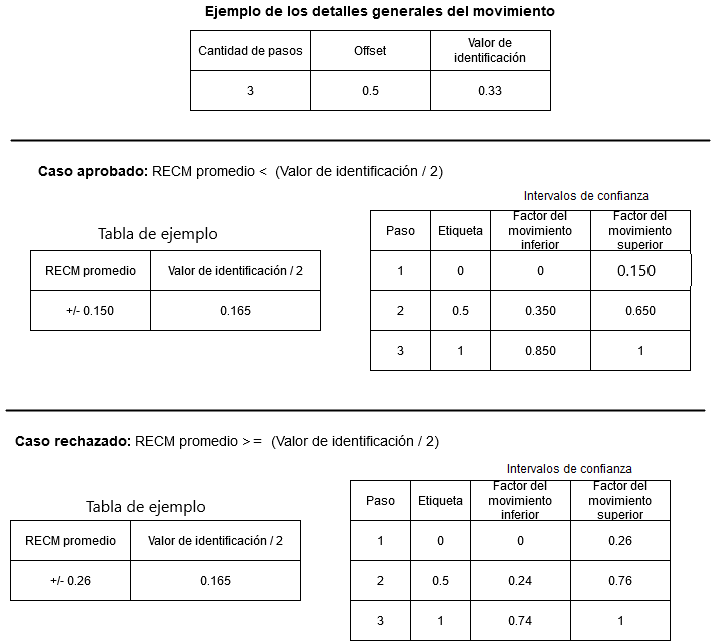
\includegraphics[width=430px,height=360px]{graphics/CriterioAceptacion.png} \\
	\textbf{Fuente:} Propia
\end{figure}
En la figura \ref{fig:AproveOrDennie}, se separa en tres partes:
\begin{itemize}
\item \textbf{Detalles generales del movimiento:} Muestra las variables num\'ericas de un movimiento.
\item \textbf{Caso aprobado:} Al construir los intervalos de confianza, se observa que no colisiona entre s\'i.
\item \textbf{Caso rechazado:} Al construir los intervalos de confianza, se observa que los intervalos del paso 1 colisiona con el paso 2 (debido que el intervalo de confianza inferior del paso 2 se encuentra dentro del intervalo de confianza del paso 1), y los intervalos del paso 2 colisiona con el paso 3 (debido que el intervalo de confianza inferior del paso 3 se encuentra dentro del intervalo de confianza del paso 2).
\end{itemize}
Adem\'as, por cada modelo aprobado se debe encontrar los intervalos de confianza  que permite detectar los pasos de un movimiento v\'alido:
\begin{formula}[H]
	\centering
	\caption{Intervalos de confianza de reconocimiento de un paso}
	\label{frm:rangoConfiabilidad}
	\begin{equation}
\begin{matrix}

intervalo\: de\: confianza = ic =[[inferior,superior]] \\
\\
ic(paso)=\left\{\begin{matrix}
inferior(paso)=\left\{\begin{matrix}
0 & si\, es\, el\, primer\, paso\\ \\ 
etiqueta(paso)- RECM_{muestra\, total} & si\: es\: paso\: intermedio \\ 
\\
1-RECM_{muestra\, total}& si\, es\, el\, \acute{u}ltimo\, paso
\end{matrix}\right. \\ 
\\ 
inferior(paso)=\left\{\begin{matrix}
RECM_{muestra\, total}& si\, es\, el\, primer\, paso \\
\\
etiqueta(paso)+RECM_{muestra\, total} & si\: es\: paso\: intermedio \\ \\ 
1 & si\: es\: el\: \acute{u}ltimo\: paso
\end{matrix}\right.
\end{matrix}\right.
\end{matrix}
	\end{equation}
	\textbf{Fuente:} Propia.
\end{formula} 
Por otro lado, se debe determinar el valor de recognition, n\'umero porcentual que determina el porcentaje de detecci\'on similar al fotograma de cada paso respectivo, es decir:
 \begin{itemize}
\item \textbf{Porcentaje mayor a cero:} Entre m\'as cercano al 100\%, el factor de movimiento es similar al valor de etiquetado (menor error).
\item \textbf{Porcentaje menor o igual a cero:} Son modelos rechazado, debido que el error es grande y adem\'as no detecta los pasos de un movimiento (por colisiones de los intervalos de confianza).
\end{itemize}
\begin{formula}[H]
	\centering
	\caption{Valor de recognition}
	\label{frm:Recognitiona}
	\begin{equation}
recognition=1-no\,v\acute{a}lidos=1-\frac{RECM_{muestra\, total}}{valor\: de\: identificaci\acute{o}n}  
	\end{equation}
	\textbf{Fuente:} Propia.
\end{formula}
\subsection{Algoritmo clasificador de un movimiento v\'alido}\label{dis:algoritmoDet}
Se presenta el algoritmo clasificador de repetici\'on de un movimiento v\'alido:
\begin{itemize}
\item Entradas:
\begin{itemize}
\item \textbf{Paso siguiente:} Variable que lleva el control del orden de todos los pasos detectados.
\item \textbf{Factor del movimiento:} Variable que indica la transici\'on del movimiento a partir del algoritmo Random Forest Regression.
\item \textbf{Paso detectado:} Variable que indica el paso actual del factor del movimiento.
\item \textbf{Paso no detectado:} Variable que no tiene un valor al inicio, la cual se asigna un valor en el caso que sea una repetici\'on inv\'alida (indica el paso del fallo del movimiento).
\end{itemize}
\item Procesos:
\begin{enumerate}[1.]
\item Asignar el paso siguiente como paso inicial (paso No.1), debido que marca el inicio de la repetici\'on. %1
\item Capturar un nuevo fotograma del Kinect, y obtiene el factor del movimiento del respectivo fotograma, a partir del algoritmo Random Forest Regression y la herramienta, Visual Gesture Builder. %2
\item Verificar si el factor del movimiento se encuentra en alg\'un intervalo de confianza para obtener el paso detectado, en caso que no se encuentre, no devolver\'a ning\'un valor.  %3
\item Verificar si el paso detectado tiene un valor, adem\'as de chequear que no sea un valor anterior (valor anterior del paso siguiente), en caso que no cumpla ambas condiciones, se debe esperar a capturar un nuevo fotograma (Volver al proceso No.2). %4
\item Verificar si el paso detectado es igual al paso siguiente, en caso que sea diferente se detect\'o una repetici\'on inv\'alida (saltar al proceso No. 9). %5
\item Verificar si el paso detectado es el \'ultimo paso, en caso contrario (saltar al proceso No. 8) %6
\item Finalizar algoritmo con repetici\'on v\'alida. %7 
\item Incrementar el paso siguiente y volver a obtener un nuevo fotograma del Kinect (saltar al proceso No. 2). %8
\item Asignar el paso no detectado como paso siguiente.
\item Finalizar el algoritmo con repetici\'on inv\'alida.
\end{enumerate}
\item Salidas:
\begin{itemize}
\item \textbf{Repetici\'on v\'alida:} El usuario pas\'o por todos los pasos de un movimiento v\'alido de forma ordenada.
\item \textbf{Repetici\'on inv\'alida y su paso no detectado:} El usuario se salt\'o el paso no detectado, lo cual genera un movimiento inv\'alido.
\end{itemize}
\end{itemize}
\begin{figure}[H]
	\caption{Algoritmo clasificador de repetici\'on de un movimiento v\'alido }
	\label{fig:capturaDatos}
	\centering
	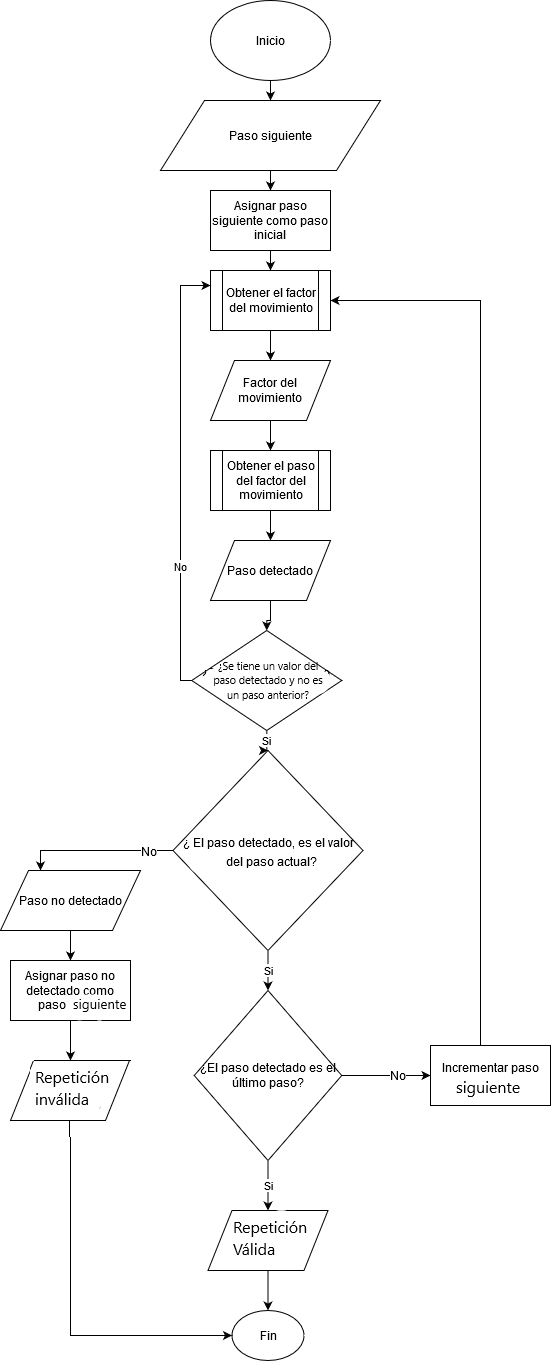
\includegraphics[width=430px,height=630px]{graphics/flujoGramaRepiticion.png} \\
	\textbf{Fuente:} Propia.
\end{figure}
Este algoritmo es aplicado para analizar los v\'ideos de testeos, debido que se etiquetaron  repeticiones de movimientos v\'alidos.  Sin embargo, al comparar los factores del movimiento de los fotogramas (de los v\'ideos de testeos), pueden ocurrir que no reconozca un paso, por lo tanto la repetici\'on del movimiento v\'alido se convierte en inv\'alido:
 \begin{figure}[H]
	\caption{Clasificaci\'on de repeticiones de movimiento v\'alido o inv\'alido  en un v\'ideo de testeo}
	\label{fig:detValido}
	\centering
	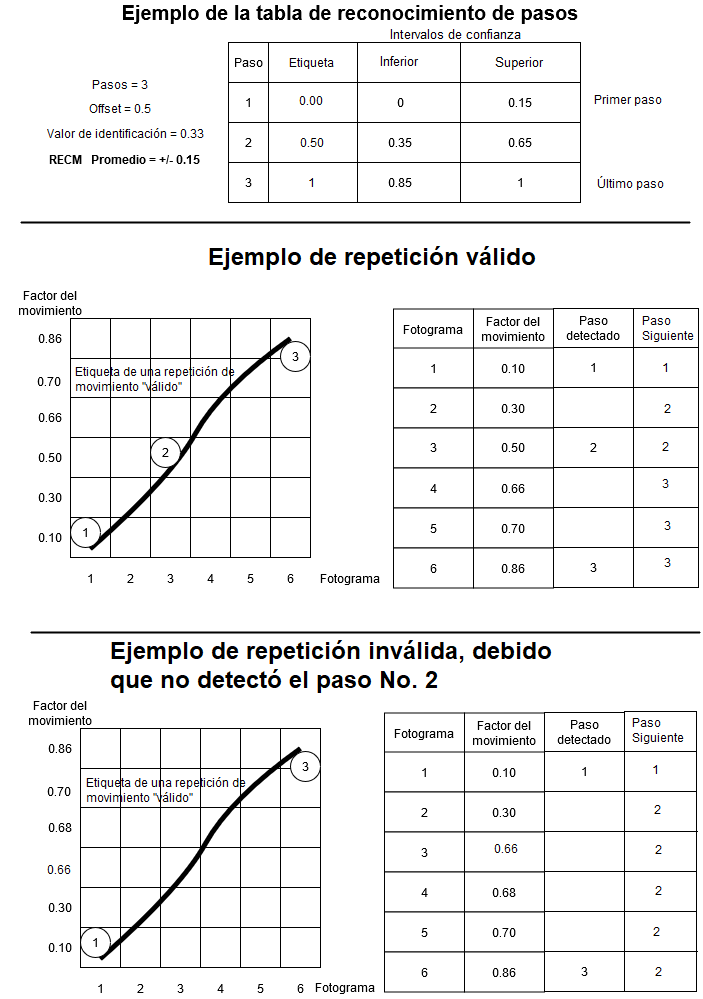
\includegraphics[width=430px,height=450px]{graphics/reconocimientoDePasos.png} \\
	\textbf{Fuente:} Propia.
\end{figure}
En la figura \ref{fig:detValido}, se divide en tres partes:
\begin{itemize}
\item \textbf{Intervalos de confianza:} Tabla que permite reconocer los pasos del movimiento, si el factor del movimiento se encuentra dentro del intervalo de confianza.
\item \textbf{Repetici\'on v\'alida:} Es v\'alido,  ya que detecta todos los pasos de manera ordenada  durante los fotogramas: Uno, tres y seis (observe que los factores del movimiento se encuentran dentro del alg\'un intervalo de confianza). 
\item \textbf{Repetici\'on inv\'alida:} Es inv\'alido, debido que para el fotograma 6, se esperaba detectar el paso dos (paso siguiente), pero se detect\'o el paso tres, por lo tanto el algoritmo determina que es una repetici\'on inv\'alida.
\end{itemize}
Este procedimiento permite completar la tabla de observaciones de clasificaci\'on de cada v\'ideo de testeo (ver anexos, tabla \ref{tab:DetectarPasoCorrecto}), en donde por cada repetici\'on etiquetada se verifica todos los pasos, por medio de tres valores:
\begin{itemize}
\item \textbf{Verdadero:} Si se detect\'o el paso correspondiente (de manera ordenada).
\item \textbf{Falso:} Repetici\'on invalida debido que no se detect\'o el paso correspondiente. 
\item \textbf{Sin valor:} El algoritmo no determin\'o ning\'un valor, debido que finaliz\'o al momento  que detect\'o una repetici\'on inv\'alida.
\end{itemize}
Por otra parte, se puede determinar el porcentaje de v\'alido e inv\'alidos del modelo de clasificador de repeticiones, adem\'as de determinar el porcentaje de cada paso no detectado:
\begin{formula}[H]
	\centering
	\caption{Porcentajes del modelo de clasificador}
	\label{frm:porcentajeClasificador}
	\begin{equation}
\begin{matrix}
repeticiones\: v\acute{a}lidas = contarSi(\acute{u}ltimo\: paso\: es\: verdadero) \\ 
 \\ 
repeticiones\: inv\acute{a}lidas = repeticiones\; totales\: del\: video - repeticiones\: v\acute{a}lidas\\ 
 \\ 
\%_{v\acute{a}lidos}=\frac{repeticiones\: v\acute{a}lidas}{repeticiones\; totales\: del\: video}\\ 
\\
\%_{inv\acute{a}lidos}=\frac{repeticiones\: inv\acute{a}lidas}{repeticiones\; totales\: del\: video}\\ 
\\ 
\%_{paso\; no\; detectado}=\frac{contarSi(paso\: es\: falso)}{repeticiones\: inv\acute{a}lidas}\\ 
\end{matrix}
	\end{equation}
	\textbf{Fuente:} Propia.
\end{formula}
Es importante saber si el modelo de clasificaci\'on  de un movimiento v\'alido se aprueba, por lo tanto se debe calcular los porcentajes de referencias v\'alido e inv\'alido, que se determinan a partir del peor de los casos (detecta una repetici\'on v\'alida y las posibles combinaciones de una  repetici\'on inv\'alida): 
 \begin{figure}[H]
	\caption{Porcentajes de referencias v\'alidos e inv\'alidos }
	\label{fig:porcValido}
	\centering
	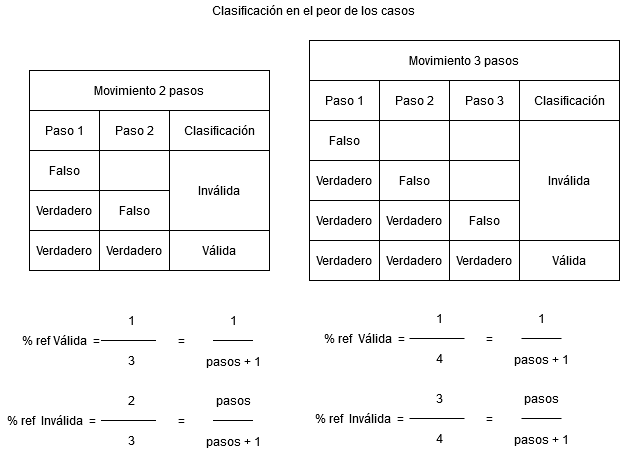
\includegraphics[width=430px,height=300px]{graphics/porceRef.png} \\
	\textbf{Fuente:} Propia.
\end{figure}
A partir de los porcentajes de referencias de clasificaci\'on, se pueden presentar dos casos:
\begin{itemize}
\item \textbf{Clasificaci\'on Aceptable:} Si el porcentaje de detecci\'on v\'alida es mayor al porcentaje de referencia v\'alida (Por consiguiente el porcentaje de detecci\'on inv\'alida es menor al porcentaje de referencia inv\'alida).
\item \textbf{Clasificaci\'on no aceptable:} Si el porcentaje de detecci\'on v\'alida es menor o igual al porcentaje de referencia v\'alida (Por consiguiente el porcentaje de detecci\'on inv\'alida es mayor o igual al porcentaje de referencia inv\'alida). 
\end{itemize}
\subsection{Dise\~no de los resultados de una rutina tabata} \label{dis:results}
En esta secci\'on se determina los resultados de la rutina de tabata, dichos resultados son encontrados a partir del seguimiento del esqueleto, la cual proporciona informaci\'on de las variables de los detalles del paso y repetici\'on (Ver f\'ormula \ref{frm:MatrizDatosRepeticion}), con el fin objetivo de encontrar la siguiente informaci\'on:
\begin{itemize}
\item \textbf{Volumen de repeticiones:} Sumatoria de las cantidades totales de repeticiones de una serie.  
\begin{code}[H]
	\caption{Pseudoc\'odigo para obtener las repeticiones totales de una rutina}
	\label{code:getRepetitions}
	\begin{lstlisting}
Entradas:
	Series de repeticiones del movimiento
	Contador de Repeticiones

Procesos:
	Recorrer cada serie de repeticiones del movimiento:
		Contar las repeticiones de la serie
		Sumar al contador de repeticiones

Salida:
	Contador de repeticiones
	\end{lstlisting}
	\textbf{Fuente:} Propia.
\end{code}

\item \textbf{Duraci\'on:} Tiempo total que se emplea en una rutina, tomando en cuenta todas las series de trabajos y descansos.
\begin{formula}[H]
	\centering
	\caption{C\'alculo de la duraci\'on de tiempo de una rutina}
	\label{eq:DurationTime}
	\begin{equation}
	Duration = \sum_{i=0}^{series}restTime +\sum_{i=0}^{series}workTime = series(restTime+workTime)
	\end{equation}
		\textbf{Fuente:} Elaborado por el autor de tesis
\end{formula}
\item \textbf{Resistencia:} Construye la estructura de la gr\'afica de la resistencia de un atleta durante una rutina a partir del recorrido de todas la series, posteriormente en cada serie se recorre todas las repeticiones y luego en cada repetici\'on se almacena el tiempo acumulado de la rutina y la cantidad de repeticiones que lleva el atleta a ese momento.
\begin{code}[H]
	\caption{Pseudoc\'odigo para crear la gr\'afica de resistencia}
	\label{code:getEndurance}
	\begin{lstlisting}
Entradas:
	Series de repeticiones del movimiento
	Gráfico en donde almacena
		Subgráfico que está compuesto por
			Nombre de la serie
			Listado de puntos en donde cada punto
				Guarda el tiempo (eje x)
				Guarda el numero de repetición (eje y)
	
Proceso:
	Crear gráfico
	Recorrer cada serie de repeticiones del movimiento
		Crear subgráfico
		Obtener el número de serie
		Crear el listado de puntos
		Recorrer cada repetición de la serie
			Obtener el número de repeticiones acumuladas 
			Obtener el tiempo del paso final de la repetición
			Crear un punto
			Guardar punto en el listado de puntos
		Almacenar en el subgráfico el número de serie y listado de puntos
		Guardar subgráfico en el listado que tiene el gráfico

Salida:
	Gráfico de resistencia
	\end{lstlisting}
	\textbf{Fuente:} Propia.
\end{code} 

\item \textbf{Potencia:} Resultado que muestra la cantidad m\'axima de repeticiones en el menor tiempo posible, la cual se encuentra a partir del recorrido de las series, luego en cada serie se determina la cantidad de repeticiones totales y el tiempo acumulado de la \'ultima repetici\'on, encontrando: 
	\begin{itemize}
	\item Una mayor cantidad de repeticiones almacenada anteriormente
	\item La misma cantidad de repeticiones almacenada anteriormente, pero se verifica si el tiempo acumulado es menor.
	\end{itemize}
\begin{code}[H]
	\caption{Pseudoc\'odigo para obtener la potencia}
	\label{code:getEndurance}
	\begin{lstlisting}
Entradas:
	Series de repeticiones del movimiento
	Potencia en donde almacena
		Cantidad de repeticiones acumuladas de una serie
		Tiempo total de la última repetición de la serie
		
Procesos:
	Crear potencia
	Recorrer cada serie de repeticiones del movimiento
		Obtener la última repetición de la serie
			Obtener el número de repeticiones acumuladas
			Obtener el tiempo del paso final de la repetición
			¿El número de repeticiones acumuladas aumentó?
				Si
					Almacenar los datos en potencia
				Sino si, ¿El número de repeticiones permaneció igual?:
					¿El Tiempo total disminuyó?:
						Si
							Almacenar los datos en potencia
						
Salida:
	Potencia 
	\end{lstlisting}
	\textbf{Fuente:} Propia.
\end{code} 

\item \textbf{Velocidad}: Raz\'on de cambio separado por:
	\begin{itemize}
	\item \textbf{Repeticiones por serie:} Variable que se determina a partir del promedio total de repeticiones por serie.
		\item \textbf{Tiempo por repetici\'on:} Variable que se determina a partir del promedio de la diferencia entre el tiempo del paso final y tiempo del paso inicial (tiempo de una repetici\'on) de cada repetici\'on realizada por el atleta.
	\end{itemize}
\end{itemize}


\begin{code}[H]
	\caption{Pseudoc\'odigo para obtener las velocidades de las rutinas}
	\label{code:getTimeOfRepetitions}
	\begin{lstlisting}
Entradas:
	Series de repeticiones del movimiento
	Velocidad en donde almacena
		Repeticiones por serie
		Tiempo por serie
		
Proceso:
	Crear velocidad
	Crear un listado de tiempos de repeticiones
	Crear un listado de repeticiones de series
	Recorrer cada serie de repeticiones del movimiento
		Obtener el total de repeticiones de la serie
		Agregar al listado de repeticiones de series
		Recorrer cada repetición de la serie
			Obtener el tiempo del paso inicial de la repetición
			Obtener el tiempo del paso final de la repetición
			Encontrar la diferencia de tiempos del paso final e inicial
			Almacenar en el listado de tiempos de repeticiones
	Encontrar el promedio de repeticiones de series
	Transformar a número entero el promedio de repeticiones de series
	Encontrar el promedio de tiempos de repeticiones
	Almacenar ambos promedios en velocidad
	
Salida:
	Velocidad
	\end{lstlisting}
	\textbf{Fuente:} Propia.
\end{code} 
\section{Criterios del proyecto}\label{criter}
En esta secci\'on se presenta todos los criterios que se siguieron para crear el modelo de reconocimientos de movimientos:
\subsection{Criterios de selecci\'on de movimiento}
\begin{itemize}
	\item El investigador y el entrenador de cada deporte  seleccionaron aquellos movimientos que se ejecutan dentro del \'area de visi\'on del sensor Kinect.
	\item El movimiento no debe ser complejo, es decir que cualquier persona pueda realizar dicho movimiento, sin importar su nivel deportivo.
	\item Debe ser un movimiento que se emplea constantemente en el deporte, para aprender nuevos movimientos complejos.
\end{itemize}
\subsection{Criterios de an\'alisis de movimiento}
\begin{itemize}
	\item Cada movimiento debe tener una articulaci\'on de an\'alisis.
	\item El conjunto de articulaciones que interact\'uan en el movimiento, se debe seleccionar con base a la separaci\'on del cuerpo humano, es decir, la parte inferior (Articulaciones abajo de la cadera central) o superior (Articulaciones arriba de la cadera central).
\end{itemize}
\subsection{Criterios de etiquetaci\'on de movimiento}
\begin{itemize}
	\item Cada repetici\'on del movimiento debe pasar por todos los pasos.
	\item El rango de etiquetaci\'on debe estar entre valores de 0 (paso inicial) y 1 (paso final).
	\item La curva de aprendizaje de cada repetici\'on, debe ser similar a una gr\'afica de forma en ese "s".
	\item No se etiqueta los datos de ruidos durante una repetici\'on del movimiento (e.g. Interrupciones, errores en el seguimiento del esqueleto).
\end{itemize}
\subsection{Criterios de error del modelo}
\begin{itemize}
	\item Se debe calcular la dispersi\'on entre los datos de la muestra y su media, a partir de la ra\'iz del error cuadr\'atico medio (RECM).
	\item Se debe calcular la dispersi\'on entre los datos reales y pronosticado a partir de la desviaci\'on media absoluta (DMA). 
	\item El error se encuentra en un rango de 0 a 1.
\end{itemize}
\subsection{Criterios de selecci\'on del modelo}
\begin{itemize}
	\item Se selecciona el submodelo que contenga la  menor RECM, en caso que exista RECM iguales, se escoge el modelo que tenga la menor DMA.
\end{itemize}
\subsection{Criterios de aceptaci\'on del modelo}
\begin{itemize}
	\item El modelo seleccionado debe considerar los errores de todas las muestras, a partir del promedio de errores de los submodelos comparados.
	\item Se aprueba el modelo, s\'i el valor promedio de la RECM es menor a un medio del valor de  identificaci\'on.
\end{itemize}
\chapter{PRESENTACI�N Y AN�LISIS DE RESULTADOS}
\section{Selecci\'on del movimiento de cada equipo deportivo} \label{res:idMov}
\begin{figure}[H]
	\caption{Formulario de movimiento de tenis de mesa}
	\label{fig:frmMovTen}
	\centering
	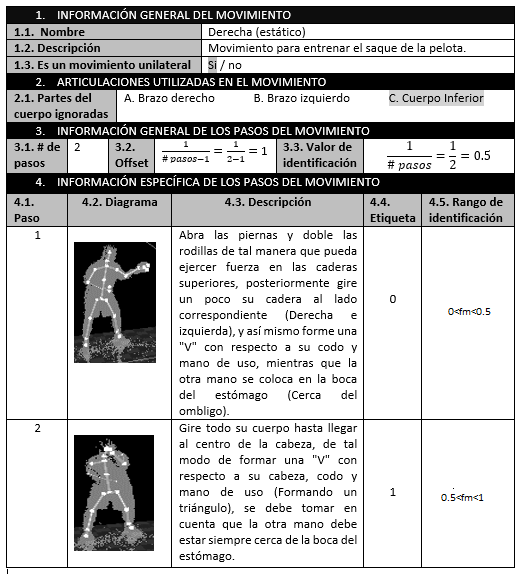
\includegraphics[width=430px,height=360px]{graphics/resultados/movimientoTenis.PNG} \\
	\textbf{Fuente:} Elaborado por el autor de tesis en base a las observaciones del trabajo de campo
\end{figure}
\begin{figure}[H]
	\caption{Formulario de movimiento de animaci\'on}
	\label{fig:frmMovCheer}
	\centering
	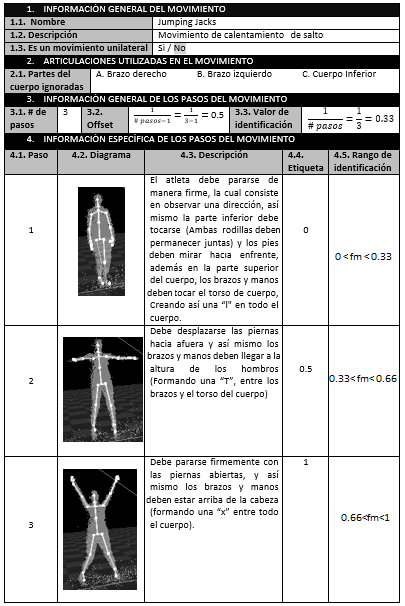
\includegraphics[width=445px,height=600px]{graphics/resultados/movimientoCheerleader.PNG} \\
	\textbf{Fuente:} Elaborado por el autor de tesis en base a las observaciones del trabajo de campo
\end{figure}
\begin{figure}[H]
	\caption{Formulario de movimiento taekwondo}
	\label{fig:frmWhiteMov}
	\centering
	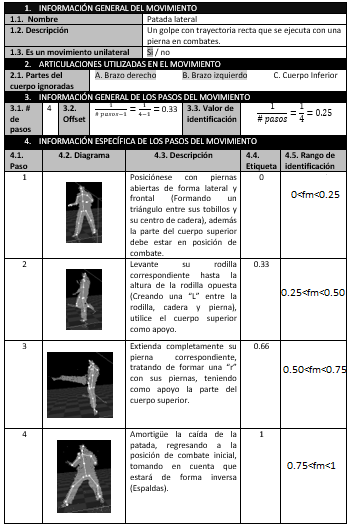
\includegraphics[width=445px,height=600px]{graphics/resultados/movimientoTaekwondo.PNG} \\
	\textbf{Fuente:} Elaborado por el autor de tesis en base a las observaciones del trabajo de campo
\end{figure}
\section{Creaci\'on de rutina del movimiento de cada equipo deportivo} \label{res:idMov}
\begin{figure}[H]
	\caption{Formulario de rutina de animaci\'on}
	\label{fig:frmRoutCher}
	\centering
	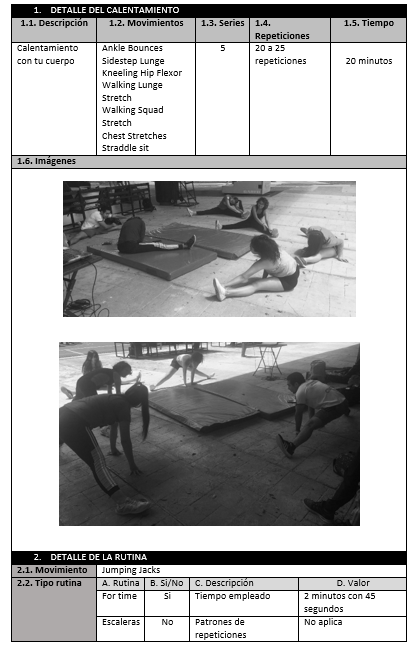
\includegraphics[width=445px,height=550px]{graphics/resultados/rutina-cheerleaders.PNG} \\
	\textbf{Fuente:} Elaborado por el autor de tesis en base a las observaciones del trabajo de campo
\end{figure}
\begin{figure}[H]
	\caption{Formulario de rutina de tenis de mesa}
	\label{fig:frmRoutTen}
	\centering
	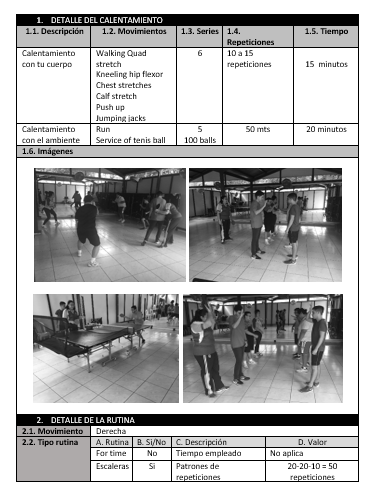
\includegraphics[width=445px,height=600px]{graphics/resultados/rutina-tennis.PNG} \\
	\textbf{Fuente:} Elaborado por el autor de tesis en base a las observaciones del trabajo de campo
\end{figure}
\begin{figure}[H]
	\caption{Formulario de rutina de taekwondo}
	\label{fig:frmRoutTaek}
	\centering
	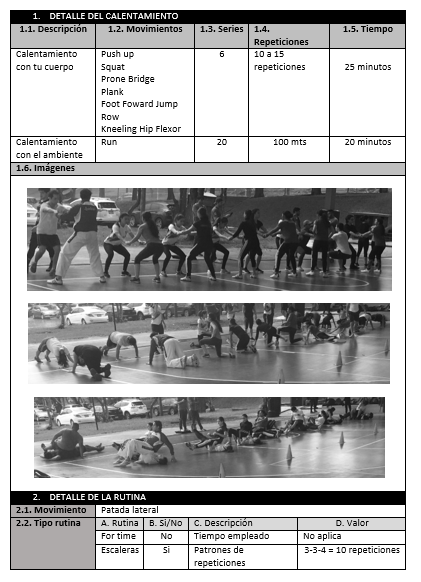
\includegraphics[width=445px,height=600px]{graphics/resultados/rutina-taekwondo.PNG} \\
	\textbf{Fuente:} Elaborado por el autor de tesis en base a las observaciones del trabajo de campo
\end{figure}
\section{Distancias de profundidad recomendadas entre el atleta y el sensor} \label{res:idMov}
\begin{table}[H]
\begin{center}
\caption{Distancias de profundidad con respecto a la cadera central del atleta, tomada a una altura del Kinect de 0.70 mts (Medida a partir del suelo)}
\label{tab:depthCalculation}
\begin{tabular}{lllll}
\hline
\multicolumn{3}{|c|}{Caracter\'isticas generales} & \multicolumn{2}{l|}{\begin{tabular}[c]{@{}l@{}}Distancia de profundidad\\ recomendada entre el \\ usuario y el sensor\end{tabular}} \\ \hline
\multicolumn{1}{|l|}{Deporte} & \multicolumn{1}{l|}{\begin{tabular}[c]{@{}l@{}}Altura promedio\\ (Metros)\end{tabular}} & \multicolumn{1}{l|}{\begin{tabular}[c]{@{}l@{}}Desviaci\'on est\'andar\\ de la altura (metros)\end{tabular}} & \multicolumn{1}{l|}{\begin{tabular}[c]{@{}l@{}}M\'inima\\ (Metros)\end{tabular}} & \multicolumn{1}{l|}{\begin{tabular}[c]{@{}l@{}}M\'axima\\ (Metros)\end{tabular}} \\ \hline
\multicolumn{1}{|l|}{Tenis de mesa} & \multicolumn{1}{l|}{1.302435} & \multicolumn{1}{l|}{0.088683} & \multicolumn{1}{l|}{3.505103} & \multicolumn{1}{l|}{3.990376} \\ \hline
\multicolumn{1}{|l|}{Animaci\'on} & \multicolumn{1}{l|}{1.342471} & \multicolumn{1}{l|}{0.059301} & \multicolumn{1}{l|}{2.763813} & \multicolumn{1}{l|}{3.411942} \\ \hline
\multicolumn{1}{|l|}{Taekwondo} & \multicolumn{1}{l|}{1.373372} & \multicolumn{1}{l|}{0.098490} & \multicolumn{1}{l|}{2.556640} & \multicolumn{1}{l|}{3.869427} \\ \hline
\multicolumn{5}{l}{\textbf{Fuente:} Instrumento \ref{ins:UI:wpf}.\ref{ins:UI:wpf:depth} utilizado en los atletas de construcci\'on y pruebas (ver secci\'on \ref{sj:1t})}
\end{tabular}
\end{center}
\end{table}

\chapter{Discusi\'on}
Este proyecto de ingenier\'ia present\'o una aplicaci\'on en el \'area deportiva para medir la repetici\'on de un movimiento v\'alido por medio del estudio de la coordinaci\'on, habilidad f\'isica que permite al atleta combinar dos o m\'as pasos requeridos para ejecutar el movimiento. 
\medbreak
La coordinaci\'on fue medida a trav\'es del factor del movimiento, variable de estudio que representa la transici\'on del movimiento en un valor num\'erico que es obtenida a partir de la etiquetaci\'on de fotogramas de cada paso del movimiento, con la herramienta de Visual Gesture Builder.
\medbreak
Esta herramienta es una caja negra, la cual recibe como datos de entradas los fotogramas etiquetados y como salida proporciona una base de datos de gesturas encriptada (.gdb), que es utilizada por una biblioteca de enlace din\'amico (DLL) del Kinect, que implementa el algoritmo Random Forest Regression.
\medbreak
En cuanto a los fotogramas, son grabados en v\'ideos por la herramienta Kinect studio. Esta herramienta permite grabar distintos monitores del Kinect, entre ellos se utilizaron el monitor de infrarrojo (para detectar los objetos) y los monitores del cuerpo humano (para detectar el seguimiento del esqueleto).
\medbreak
Cada v\'ideo consiste en grabar atletas, ejecutando repeticiones del movimiento v\'alidos de acuerdo con los criterios del profesional (dentro del rango de distancias de profundidades), con el fin objetivo de proporcionar distintos fotogramas de un paso de un movimiento v\'alido (tal como se observa en los resultados de fotogramas del movimiento).
\medbreak
As\'i mismo el profesional tiene un papel importante en el proyecto, debido que estableci\'o los pasos que deben seguir el movimiento. Y al mismo tiempo, conoce las habilidades f\'isicas de cada atleta, permitiendo saber el n\'umero de repeticiones v\'alidas que puede ejecutar cada atleta (tal como se observa en los resultados de proceso de etiquetaci\'on de un movimiento).
\medbreak
En cuanto al n\'umero de atletas de entrenamiento y testeo, el investigador utiliz\'o solo un v\'ideo de testeo y los dem\'as v\'ideos se utilizaron para el entrenamiento del modelo, sin embargo, este criterio puede ser modificado para futuros trabajos, seleccionando la muestra de testeos de un atleta profesional (mejor de los casos), un atleta regular (caso medio) y un nuevo atleta (peor de los casos).
\medbreak
Por otra parte, la muestra se considera peque\~na con relaci\'on a las cantidades de datos que utilizaron en los trabajos relacionados, por lo tanto, para resolver este problema se utiliz\'o la validaci\'on cruzada 3-Fold, que permite crear 3 submodelos con distintas combinaciones de datos de entrenamientos y testeos (creadas a partir de la muestra), con la finalidad de observar como se comporta el modelo con distintos datos.
\medbreak
Con respecto a la etiquetaci\'on de fotogramas de un movimiento v\'alido, el investigador estableci\'o que para el paso inicial tendr\'a un valor de cero y para el paso final tendr\'a un valor uno, de modo que facilita etiquetar los pasos intermedios por partes iguales (valor offset), y por otro lado permite crear rangos iguales para identificar cada paso (valor de identificaci\'on).
\medbreak
Por cada submodelo se etiquet\'o los fotogramas de los videos de entrenamiento para obtener su base de datos de gesturas, posteriormente esa base de datos fue utilizada en la secci\'on de an\'alisis de Visual Gesture Builder, que permite comparar el valor etiquetado (valor esperado) y el factor del movimiento por fotograma (valor obtenido), de manera de obtener el error del factor del movimiento.
\medbreak
El modelo seleccion\'o el submodelo que tenga la menor desviaci\'on del factor del movimiento con respecto a la etiqueta (RECM), en caso de que exista m\'as submodelos con el mismo valor de RECM, se selecciona el submodelo que tenga la menor dispersi\'on del factor del movimiento (MAD).
\medbreak
La desviaci\'on del factor del movimiento con respecto a la etiqueta es un error importante en el proyecto, ya que a partir de ello se construye los intervalos de confianza para reconocer los pasos requeridos de un movimiento, de modo que se cre\'o el criterio de aceptaci\'on del modelo para evitar que los intervalos de confianza de los pasos intermedios colisionen con otros intervalos.
\medbreak
El modelo de taekwondo es rechazado por que no cumple con el criterio de aceptaci\'on, y esto es debido por su gran error, que puede ser a dos causas:
\begin{enumerate}[1.]
\item El tama\~no de la muestra es peque\~na comparada con las muestras de animaci\'on y tenis de mesa (modelos aceptados).
\item Durante los fotogramas del paso dos y tres (de una patada lateral), el seguimiento del esqueleto no concuerda con la sombra del atleta.
\end{enumerate}
Por otra parte, la certeza de los modelos aceptados est\'a dado por su recognition, valor porcentual que determina que tan parecidos son los fotogramas dentro del intervalo de confianza con respecto al fotograma de cada paso (valor esperado). Tal como se observa en los resultados, el equipo de animaci\'on tiene un 82.96\% de recognition (Valor cercano al 100\%), lo cual reconoce fotogramas que tienen peque\~nos desplazamientos en los pies y brazos, mientras que para el equipo de tenis de mesa tiene un recognition de 52.08\%  (Valor alejado al 100\%), donde reconoce fotogramas que tienen mayores desplazamientos en todas las articulaciones.
\medbreak
As\'i mismo, el modelo de reconocimiento de cada paso funciona \'unicamente con el movimiento que fue entrenado y testeado, esto quiere decir que el modelo de reconocimiento de pasos jumping jacks no reconoce los pasos de un saque derecha, y viceversa (tal como se muestra en el cuadro comparativo entre un jumping jack  y saque derecha).
\medbreak
En cuanto al algoritmo clasificador del movimiento v\'alido, chequea todos los fotogramas capturados por el sensor Kinect, en donde por cada fotograma obtiene el factor del movimiento, a partir del algoritmo, Random Forest Regression, posteriormente examina si el factor del movimiento se encuentra en un intervalo de confianza para detectar el paso. Finalmente, estos procesos se repiten hasta verificar que sea una repetici\'on de un movimiento v\'alido (detect\'o todos los pasos del movimiento de manera ordenada) o una repetici\'on de un movimiento inv\'alido (indicando el paso que no se detect\'o).
\medbreak
Este algoritmo clasificador se aplic\'o a cada v\'ideo de testeo, para clasificar todas las repeticiones de los atletas de acuerdo a los intervalos de confianza de detecci\'on de cada paso, por consiguiente se calcul\'o el porcentaje de clasificaci\'on v\'alidas e inv\'alidas y as\'i mismo se calcul\'o los porcentajes de cada paso no detectado (En las repeticiones inv\'alidas), tal como se observa en los resultados:
\begin{itemize}
\item	De acuerdo al algoritmo clasificador, las animadoras de testeos realizaron un 49.43\% de repeticiones inv\'alidas de jumping jacks, debido que durante varias repeticiones fallaron en el paso tres (70.93\%) o pocas veces fallaron en el paso dos (29.07\%).
\item De acuerdo al algoritmos clasificador, Los jugadores de testeos de tenis de mesa realizaron un 34.69\% de repeticiones inv\'alidas de saques derecha, debido que durante varias repeticiones fallaron en el paso dos (82.35\%) o rara vez fallaron en el paso uno (17.65\%).
\end{itemize}
Los porcentajes de clasificaci\'on se compara con los porcentajes de referencias en el peor de los casos, la cual se conforma por todas las posibles combinaciones que se puede dar una repetici\'on inv\'alida y el caso de una repetici\'on v\'alida, de modo que es aceptable si el porcentaje v\'alida real es mayor al porcentaje de referencia v\'alida y por ende el porcentaje inv\'alida real es menor al porcentaje de referencia inv\'alida.
\medbreak
En cuanto al proceso de validaci\'on del modelo de detecci\'on de pasos y el algoritmo de clasificaci\'on de movimientos v\'alidos, se utilizaron atletas que no participaron en el proceso de entrenamiento y testeo. As\'i mismo, el profesional le program\'o a cada atleta una rutina tabata de dos series de 40 segundos de trabajo y 20 segundos de descanso, con la finalidad de validar ambos elementos (detecci\'on de paso y clasificaci\'on de movimiento v\'alido). Al finalizar cada rutina se le proporcion\'o los resultados de las repeticiones v\'alidas por serie de trabajo y el tiempo que ejecuta una repetici\'on v\'alida (ambos resultados miden la habilidad f\'isica, velocidad). 
\medbreak
Para verificar que el algoritmo clasificador funcione en el proceso de validaci\'on, se realiz\'o un pron\'ostico donde los atletas ejecutan constantemente la repetici\'on m\'as larga de la muestra de entrenamiento y testeo (durante el tiempo de trabajo de tabata). Posteriormente se calcul\'o el total de repeticiones pronosticadas v\'alidas (a partir del porcentaje de movimientos v\'alidas), con el fin objetivo de comparar las repeticiones v\'alidas realizadas en el entrenamiento tabata. Como resultado, el modelo detect\'o m\'as repeticiones v\'alidas comparado con el peor de los casos.
\medbreak
En conclusi\'on, se puede afirmar la hip\'otesis del proyecto, ya que durante un entrenamiento tabata (actividad f\'isica), el modelo contabiliza las repeticiones v\'alidas durante el tiempo de trabajo, de modo que se resuelve el planteamiento del problema:
\begin{itemize}
\item	Para la primera problem\'atica, el profesional puede programar rutinas tabata que implemente el modelo clasificador de un movimiento v\'alido, con el fin objetivo que el usuario entrene el movimiento y vea su progreso por medio de las repeticiones v\'alidas.
\item	Para la segunda problem\'atica, el profesional puede programar rutinas tabata al usuario con el fin de objetivo de verificar si est\'a realizando repeticiones v\'alidas. En caso de que no contabilice, el profesional le puede ayudar al atleta a adaptar el movimiento para que pueda contabilizar la repetici\'on v\'alida.
\end{itemize}

\chapter{CONCLUSIONES FINALES DEL PROYECTO}
\section{CONCLUSIONES} \label{ded:con}
\begin{itemize}
\item De acuerdo a los tres deportes estudiados, se puede analizar movimientos que son f\'aciles de hacer dentro el campo de visi\'on del sensor Kinect.
\item Conforme a los tres movimientos analizados, se puede deducir que un movimiento esta compuesto por dos o m\'as pasos, y en cada paso se debe ejecutar  la postura correcta.
\item En relaci\'on a los entrenamientos de los deportes seleccionados, se puede concluir que el calentamiento es una actividad importante para la preparaci\'on de los movimientos que se ejecutan en una rutina.
\item Acorde a las rutinas de captura de datos utilizados en el proyecto,  se puede inferir que la rutina por tiempo, es utilizado en los atletas que puede ejecutar un mayor volumen de repetici\'on en un largo per\'iodo de tiempo (Sin importar la cantidad de repeticiones), mientras que la rutina por repeticiones (Escaleras), se establece el n\'umero de repeticiones que debe ejecutar el deportista.
\item  Con respecto al seguimiento de esqueleto de cada movimiento analizado, se puede deducir que la distancia correcta para que el sensor Kinect pueda detectar al atleta, es de  2.56 metros a 3.99 metros de profundidad. Sin embargo, el sensor debe estar a una altura de 0.70 metros (Respecto al suelo).
\item  En base a las grabaciones (Tomadas por la herramienta, Kinect Studio) durante la etapa de recolecci\'on de datos, se puede concluir que existe tres tipos de sucesos que puede generar datos inservible; la primera consta de las interrupciones de personas u objetos, adem\'as de los eventos inesperado, como la lluvia. As\'i mismo el segundo suceso se relaciona con las fallas del hardware o software que impide visualizar el seguimiento del esqueleto y finalmente el tercer evento consta en la grabaci\'on dentro de un entorno no ideal, pongamos por caso los espacios abiertos y no planos.
\item En relaci\'on a la implementaci\'on de la base de datos de reconocimiento de gesturas y posturas, se puede deducir que el software, Visual Gesture Builder (Herramienta de inteligencia artificial del SDK del Kinect), crea modelos de reconocimiento a partir de la etiquetaci\'on decimal de fotogramas, es decir por cada paso del movimiento analizado esta etiquetado con un n\'umero entre 0 a 1.
\item De acuerdo a los modelos de pron\'ostico de gesturas y  posturas, se puede concluir que el valor resultante de cada modelo se le llama, factor de movimiento, la cual puede ser comparado por el valor etiquetado de las grabaciones de pruebas, con el fin de objetivo de encontrar los errores del pron\'ostico (Diferencia entre factor movimiento y valor etiquetado).
\item Conforme a los errores de pron\'ostico de cada modelo, se determin\'o el error promedio (desviaci\'on media absoluta), as\'i mismo se construy\'o los rangos de confianza de cada paso, con la ayuda de la desviaci\'on t\'ipica del modelo (Ra\'iz del error cuadr\'atico medio).
\item Por lo que se refiere a la interfaz gr\'afica del seguimiento de esqueleto, se ha utilizado la tecnolog\'ia Windows Presentation Foundation, dado  las herramientas de dibujos (Windows media), manejos de temporizadores (Windows Threading) y manejos de los datos del sensor (SDK de Kinect).
\item En cuanto al algoritmo de detecci\'on de repetici\'on de un movimiento, se detecta \'unicamente, si el seguimiento de esqueleto del atleta pasa por todos los pasos del movimiento de manera ordenada y ascendente.
\item Por lo que se refiere a los resultados de los entrenamiento de cada movimiento estudiado, se ha deducido que la rutina Tabata permite contabilizar las repeticiones del movimiento durante los tiempos de trabajos, adem\'as de ser un entrenamiento de alta intensidad con alta metabolizaci\'on de energ\'ia (Obtenci\'on y gasto de mol\'eculas de ATP) en todo el cuerpo, durante los tiempos de trabajo y descanso.
\item De acuerdo a la comprobaci\'on del modelo de reconocimiento de cada movimiento, se ha comprobado y validado cada modelo por medio de la validaci\'on  cruzada, 3-Fold, la cual permite crear distintos modelos de reconocimiento de movimiento a partir de  combinaciones de datos de pruebas y entrenamientos.
\end{itemize}
\section{Recomendaciones} \label{ded:rec}
\begin{itemize}
\item Si se trabaja con un movimiento complejo, se recomienda analizarlo por dos o m\'as movimientos simples (divide y conquistar\'a), por ejemplo para el movimiento de patada lateral de taekwondo, se puede analizar por dos movimientos simples: Levantamiento de rodilla a la cadera (paso uno y dos) y levantamiento de pierna a la cadera (paso tres y cuatro).
\item Para disminuir el error del modelo de reconocimiento de los pasos requeridos de un  movimiento v\'alido, se recomienda recolectar m\'as  datos de  repeticiones del movimiento (realizadas por distintos atletas), tal como se muestra en los resultados, el modelo de animaci\'on tiene un error de +/-0.06  con 1229 repeticiones, posteriormente le sigue el modelo de tenis de mesa con un error de +/-0.24 con 332 repeticiones y finalmente el modelo de taekwondo tiene un error de +/-0.32 con 155 repeticiones.
\item Se sugiere capturar los datos en un  lugar que tenga un clima agradable -e.g. Sin lluvia o exceso de sol-, con un espacio suficiente para realizar el movimiento sin ninguna interrupci\'on ( por ejemplo, lugares planos), adem\'as de tener una  ventilaci\'on e iluminaci\'on correcta.
\item Se recomienda realizar un modelo de detecci\'on de los pasos requeridos de un movimiento v\'alido, por cada lugar deportivo, debido que son otros atletas, otros profesionales y otros  criterios para ejecutar un movimiento.
\end{itemize}
\backmatter
\bibliography{backmatter/bibliografia}
\appendix
\clearpage
\addappheadtotoc
\appendixpage

\end{document}